% Options for packages loaded elsewhere
\PassOptionsToPackage{unicode}{hyperref}
\PassOptionsToPackage{hyphens}{url}
%
\documentclass[
]{book}
\usepackage{lmodern}
\usepackage{amsmath}
\usepackage{ifxetex,ifluatex}
\ifnum 0\ifxetex 1\fi\ifluatex 1\fi=0 % if pdftex
  \usepackage[T1]{fontenc}
  \usepackage[utf8]{inputenc}
  \usepackage{textcomp} % provide euro and other symbols
  \usepackage{amssymb}
\else % if luatex or xetex
  \usepackage{unicode-math}
  \defaultfontfeatures{Scale=MatchLowercase}
  \defaultfontfeatures[\rmfamily]{Ligatures=TeX,Scale=1}
\fi
% Use upquote if available, for straight quotes in verbatim environments
\IfFileExists{upquote.sty}{\usepackage{upquote}}{}
\IfFileExists{microtype.sty}{% use microtype if available
  \usepackage[]{microtype}
  \UseMicrotypeSet[protrusion]{basicmath} % disable protrusion for tt fonts
}{}
\makeatletter
\@ifundefined{KOMAClassName}{% if non-KOMA class
  \IfFileExists{parskip.sty}{%
    \usepackage{parskip}
  }{% else
    \setlength{\parindent}{0pt}
    \setlength{\parskip}{6pt plus 2pt minus 1pt}}
}{% if KOMA class
  \KOMAoptions{parskip=half}}
\makeatother
\usepackage{xcolor}
\IfFileExists{xurl.sty}{\usepackage{xurl}}{} % add URL line breaks if available
\IfFileExists{bookmark.sty}{\usepackage{bookmark}}{\usepackage{hyperref}}
\hypersetup{
  pdftitle={ENGE 5714 Course Notes 2021},
  pdfauthor={Dr.~Katz},
  hidelinks,
  pdfcreator={LaTeX via pandoc}}
\urlstyle{same} % disable monospaced font for URLs
\usepackage{color}
\usepackage{fancyvrb}
\newcommand{\VerbBar}{|}
\newcommand{\VERB}{\Verb[commandchars=\\\{\}]}
\DefineVerbatimEnvironment{Highlighting}{Verbatim}{commandchars=\\\{\}}
% Add ',fontsize=\small' for more characters per line
\usepackage{framed}
\definecolor{shadecolor}{RGB}{248,248,248}
\newenvironment{Shaded}{\begin{snugshade}}{\end{snugshade}}
\newcommand{\AlertTok}[1]{\textcolor[rgb]{0.94,0.16,0.16}{#1}}
\newcommand{\AnnotationTok}[1]{\textcolor[rgb]{0.56,0.35,0.01}{\textbf{\textit{#1}}}}
\newcommand{\AttributeTok}[1]{\textcolor[rgb]{0.77,0.63,0.00}{#1}}
\newcommand{\BaseNTok}[1]{\textcolor[rgb]{0.00,0.00,0.81}{#1}}
\newcommand{\BuiltInTok}[1]{#1}
\newcommand{\CharTok}[1]{\textcolor[rgb]{0.31,0.60,0.02}{#1}}
\newcommand{\CommentTok}[1]{\textcolor[rgb]{0.56,0.35,0.01}{\textit{#1}}}
\newcommand{\CommentVarTok}[1]{\textcolor[rgb]{0.56,0.35,0.01}{\textbf{\textit{#1}}}}
\newcommand{\ConstantTok}[1]{\textcolor[rgb]{0.00,0.00,0.00}{#1}}
\newcommand{\ControlFlowTok}[1]{\textcolor[rgb]{0.13,0.29,0.53}{\textbf{#1}}}
\newcommand{\DataTypeTok}[1]{\textcolor[rgb]{0.13,0.29,0.53}{#1}}
\newcommand{\DecValTok}[1]{\textcolor[rgb]{0.00,0.00,0.81}{#1}}
\newcommand{\DocumentationTok}[1]{\textcolor[rgb]{0.56,0.35,0.01}{\textbf{\textit{#1}}}}
\newcommand{\ErrorTok}[1]{\textcolor[rgb]{0.64,0.00,0.00}{\textbf{#1}}}
\newcommand{\ExtensionTok}[1]{#1}
\newcommand{\FloatTok}[1]{\textcolor[rgb]{0.00,0.00,0.81}{#1}}
\newcommand{\FunctionTok}[1]{\textcolor[rgb]{0.00,0.00,0.00}{#1}}
\newcommand{\ImportTok}[1]{#1}
\newcommand{\InformationTok}[1]{\textcolor[rgb]{0.56,0.35,0.01}{\textbf{\textit{#1}}}}
\newcommand{\KeywordTok}[1]{\textcolor[rgb]{0.13,0.29,0.53}{\textbf{#1}}}
\newcommand{\NormalTok}[1]{#1}
\newcommand{\OperatorTok}[1]{\textcolor[rgb]{0.81,0.36,0.00}{\textbf{#1}}}
\newcommand{\OtherTok}[1]{\textcolor[rgb]{0.56,0.35,0.01}{#1}}
\newcommand{\PreprocessorTok}[1]{\textcolor[rgb]{0.56,0.35,0.01}{\textit{#1}}}
\newcommand{\RegionMarkerTok}[1]{#1}
\newcommand{\SpecialCharTok}[1]{\textcolor[rgb]{0.00,0.00,0.00}{#1}}
\newcommand{\SpecialStringTok}[1]{\textcolor[rgb]{0.31,0.60,0.02}{#1}}
\newcommand{\StringTok}[1]{\textcolor[rgb]{0.31,0.60,0.02}{#1}}
\newcommand{\VariableTok}[1]{\textcolor[rgb]{0.00,0.00,0.00}{#1}}
\newcommand{\VerbatimStringTok}[1]{\textcolor[rgb]{0.31,0.60,0.02}{#1}}
\newcommand{\WarningTok}[1]{\textcolor[rgb]{0.56,0.35,0.01}{\textbf{\textit{#1}}}}
\usepackage{longtable,booktabs}
\usepackage{calc} % for calculating minipage widths
% Correct order of tables after \paragraph or \subparagraph
\usepackage{etoolbox}
\makeatletter
\patchcmd\longtable{\par}{\if@noskipsec\mbox{}\fi\par}{}{}
\makeatother
% Allow footnotes in longtable head/foot
\IfFileExists{footnotehyper.sty}{\usepackage{footnotehyper}}{\usepackage{footnote}}
\makesavenoteenv{longtable}
\usepackage{graphicx}
\makeatletter
\def\maxwidth{\ifdim\Gin@nat@width>\linewidth\linewidth\else\Gin@nat@width\fi}
\def\maxheight{\ifdim\Gin@nat@height>\textheight\textheight\else\Gin@nat@height\fi}
\makeatother
% Scale images if necessary, so that they will not overflow the page
% margins by default, and it is still possible to overwrite the defaults
% using explicit options in \includegraphics[width, height, ...]{}
\setkeys{Gin}{width=\maxwidth,height=\maxheight,keepaspectratio}
% Set default figure placement to htbp
\makeatletter
\def\fps@figure{htbp}
\makeatother
\setlength{\emergencystretch}{3em} % prevent overfull lines
\providecommand{\tightlist}{%
  \setlength{\itemsep}{0pt}\setlength{\parskip}{0pt}}
\setcounter{secnumdepth}{5}
\usepackage{booktabs}
\usepackage{booktabs}
\usepackage{longtable}
\usepackage{array}
\usepackage{multirow}
\usepackage{wrapfig}
\usepackage{float}
\usepackage{colortbl}
\usepackage{pdflscape}
\usepackage{tabu}
\usepackage{threeparttable}
\usepackage{threeparttablex}
\usepackage[normalem]{ulem}
\usepackage{makecell}
\usepackage{xcolor}
\ifluatex
  \usepackage{selnolig}  % disable illegal ligatures
\fi
\usepackage[]{natbib}
\bibliographystyle{apalike}

\title{ENGE 5714 Course Notes 2021}
\author{Dr.~Katz}
\date{2021-02-15}

\begin{document}
\maketitle

{
\setcounter{tocdepth}{1}
\tableofcontents
}
\hypertarget{preamble}{%
\chapter*{Preamble}\label{preamble}}
\addcontentsline{toc}{chapter}{Preamble}

This book will be a living document of notes for ENGE 5714 - Quantitative Research Methods in Engineering Education. I will try to keep it updated and post alerts about updates in our course Slack workspace.

\hypertarget{week-1-introductions}{%
\chapter{Week 1: Introductions}\label{week-1-introductions}}

In week one we just reviewed some of the materials from the fall semester. By the end we discussed R and RStudio, but this first week was primarily about getting to know each other and the outline of the course.

\hypertarget{week-2-intro-stats-data-distributions-intro-r-rstudio}{%
\chapter{Week 2: Intro stats, Data \& Distributions, Intro R \& RStudio}\label{week-2-intro-stats-data-distributions-intro-r-rstudio}}

This week, we discuss some very basic ideas related to statistics, data, and working in R.

\hypertarget{first-steps-in-r}{%
\section{First steps in R}\label{first-steps-in-r}}

We can create a new variable by assigning it a value with the \texttt{\textless{}-} operator. Let's create a vector of numbers 1 to 10 with the \texttt{seq()} function and then a separate vector that takes each of the x values, multiplies it by 2, and adds 3.

\begin{Shaded}
\begin{Highlighting}[]
\NormalTok{x }\OtherTok{\textless{}{-}} \FunctionTok{seq}\NormalTok{(}\DecValTok{1}\SpecialCharTok{:}\DecValTok{10}\NormalTok{)}
\NormalTok{y }\OtherTok{\textless{}{-}} \DecValTok{2}\SpecialCharTok{*}\NormalTok{ x }\SpecialCharTok{+} \DecValTok{3}
\end{Highlighting}
\end{Shaded}

Just to make sure everything worked as expected, we can then just type \texttt{x} and \texttt{y} and R will print their values. We could also look in the ``environment'' window to see whether those variables (and their expected values) were actually created.

\begin{Shaded}
\begin{Highlighting}[]
\NormalTok{x}
\end{Highlighting}
\end{Shaded}

\begin{verbatim}
##  [1]  1  2  3  4  5  6  7  8  9 10
\end{verbatim}

\begin{Shaded}
\begin{Highlighting}[]
\NormalTok{y}
\end{Highlighting}
\end{Shaded}

\begin{verbatim}
##  [1]  5  7  9 11 13 15 17 19 21 23
\end{verbatim}

So far, so good. If we want to quickly visualize this, we could create a simple scatter plot with the \texttt{plot()} command (note: we will come back to plotting data much more in week 3).

\begin{Shaded}
\begin{Highlighting}[]
\FunctionTok{plot}\NormalTok{(x, y)}
\end{Highlighting}
\end{Shaded}

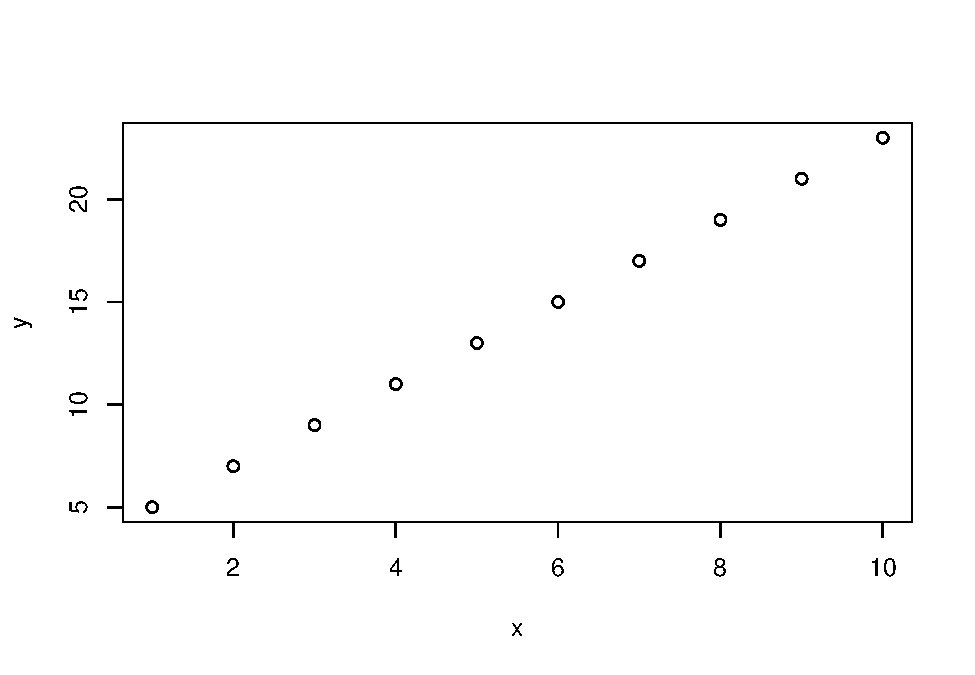
\includegraphics{test_course_notes_files/figure-latex/unnamed-chunk-3-1.pdf}

\hypertarget{getting-your-r-environment-set-up}{%
\section{Getting your R environment set up}\label{getting-your-r-environment-set-up}}

One of the first things you will have in any script or .rmd file is a section to load all the libraries that you use in that script.

You can install a library by using the install.packages() function, for example:

\texttt{install.packages("tidyverse")}, \texttt{install.packages("janitor")}, and \texttt{install.packages("psych")}

with this installed, you can then load the package using the library() function

\begin{Shaded}
\begin{Highlighting}[]
\FunctionTok{library}\NormalTok{(tidyverse)}
\end{Highlighting}
\end{Shaded}

\begin{verbatim}
## -- Attaching packages --------------------------------------------------- tidyverse 1.3.0 --
\end{verbatim}

\begin{verbatim}
## v ggplot2 3.3.2     v purrr   0.3.4
## v tibble  3.0.3     v dplyr   1.0.0
## v tidyr   1.1.0     v stringr 1.4.0
## v readr   1.3.1     v forcats 0.5.0
\end{verbatim}

\begin{verbatim}
## -- Conflicts ------------------------------------------------------ tidyverse_conflicts() --
## x dplyr::filter() masks stats::filter()
## x dplyr::lag()    masks stats::lag()
\end{verbatim}

\begin{Shaded}
\begin{Highlighting}[]
\FunctionTok{library}\NormalTok{(janitor)}
\end{Highlighting}
\end{Shaded}

\begin{verbatim}
## Warning: package 'janitor' was built under R version 4.0.3
\end{verbatim}

\begin{verbatim}
## 
## Attaching package: 'janitor'
\end{verbatim}

\begin{verbatim}
## The following objects are masked from 'package:stats':
## 
##     chisq.test, fisher.test
\end{verbatim}

\begin{Shaded}
\begin{Highlighting}[]
\FunctionTok{library}\NormalTok{(psych)}
\end{Highlighting}
\end{Shaded}

\begin{verbatim}
## 
## Attaching package: 'psych'
\end{verbatim}

\begin{verbatim}
## The following objects are masked from 'package:ggplot2':
## 
##     %+%, alpha
\end{verbatim}

\hypertarget{reading-in-data}{%
\section{Reading in data}\label{reading-in-data}}

A good first step when working in R is to check which directory you are working in with the \texttt{getwd()} function. You should get a directory in response.

\begin{Shaded}
\begin{Highlighting}[]
\FunctionTok{getwd}\NormalTok{()}
\end{Highlighting}
\end{Shaded}

\begin{verbatim}
## [1] "C:/Users/akatz4/Desktop/test_course_note"
\end{verbatim}

You can also check which files are in that directory with \texttt{list.files()}.

\begin{Shaded}
\begin{Highlighting}[]
\FunctionTok{list.files}\NormalTok{()}
\end{Highlighting}
\end{Shaded}

\begin{verbatim}
##  [1] "_book"                                                                 
##  [2] "_bookdown.yml"                                                         
##  [3] "_bookdown_files"                                                       
##  [4] "_output.yml"                                                           
##  [5] "01-Week_01.Rmd"                                                        
##  [6] "02-Week_02.Rmd"                                                        
##  [7] "03-Week_03.Rmd"                                                        
##  [8] "04-Week_04.Rmd"                                                        
##  [9] "05-Week_05.Rmd"                                                        
## [10] "06-Week_06.Rmd"                                                        
## [11] "book.bib"                                                              
## [12] "docs"                                                                  
## [13] "ENGE_5714_2021_pre_survey.csv"                                         
## [14] "Free Reduced Lunch by Schools and Grade Structures 2008-2017_final.csv"
## [15] "index.Rmd"                                                             
## [16] "packages.bib"                                                          
## [17] "preamble.tex"                                                          
## [18] "README.md"                                                             
## [19] "RExam.dat"                                                             
## [20] "seniorsurvey.csv"                                                      
## [21] "style.css"                                                             
## [22] "survey_student_info.csv"                                               
## [23] "test_course_note.Rproj"                                                
## [24] "test_course_notes.Rmd"                                                 
## [25] "test_course_notes_files"
\end{verbatim}

If you notice that the file you are looking for is not there, then you can use setwd() to change your working directory

\texttt{setwd("./Week\ 2/")}

After that, make sure you have switched to the correct working directory
\texttt{getwd()} and then \texttt{list.files()}.

Assuming you have directed yourself to the correct place, you can now read in the file(s) that you want to be working with. There are a \emph{lot} of ways to do this. Since we will be spending a lot of time in class working with .csv files, we will focus on using the \texttt{read\_csv()} function from the readr package (part of the tidyverse collection of packages). This function will read in the .csv file and store the data as a tibble (a tidyverse version of a data frame, which we can think of as a collection of observations stored in rows with values for variables for each observation stored in columns).

\begin{Shaded}
\begin{Highlighting}[]
\NormalTok{prior\_survey }\OtherTok{\textless{}{-}} \FunctionTok{read\_csv}\NormalTok{(}\StringTok{"ENGE\_5714\_2021\_pre\_survey.csv"}\NormalTok{)}
\end{Highlighting}
\end{Shaded}

\begin{verbatim}
## Parsed with column specification:
## cols(
##   .default = col_character(),
##   student_id = col_double()
## )
\end{verbatim}

\begin{verbatim}
## See spec(...) for full column specifications.
\end{verbatim}

\hypertarget{exploring-the-data}{%
\section{Exploring the data}\label{exploring-the-data}}

Now that we have loaded in the data, let's take a look at the csv. If we just run a line with the name of the tibble - i.e., \texttt{prior\_survey} then we should receive a printout that shows the first several rows of that tibble and a listing of all the columns, along with the data types (i.e., double for numeric values, character for strings, etc) of each column.

\begin{Shaded}
\begin{Highlighting}[]
\NormalTok{prior\_survey}
\end{Highlighting}
\end{Shaded}

\begin{verbatim}
## # A tibble: 24 x 49
##    student_id `I have taken a~ `I am intereste~ `I know what a ~
##         <dbl> <chr>            <chr>            <chr>           
##  1          1 Somewhat disagr~ Somewhat agree   Strongly disagr~
##  2          2 Strongly disagr~ Neither agree n~ Somewhat agree  
##  3          3 Strongly disagr~ Somewhat agree   Somewhat agree  
##  4          4 Somewhat disagr~ Strongly agree   Strongly disagr~
##  5          5 Somewhat agree   Strongly agree   Somewhat agree  
##  6          6 Somewhat disagr~ Somewhat agree   Somewhat disagr~
##  7          7 Strongly disagr~ Somewhat agree   Strongly disagr~
##  8          8 Somewhat agree   Somewhat agree   Somewhat agree  
##  9          9 Strongly disagr~ Strongly agree   Somewhat agree  
## 10         10 Neither agree n~ Strongly agree   Somewhat agree  
## # ... with 14 more rows, and 45 more variables: `I know what a type II error
## #   is` <chr>, `I know what a (statistical) confidence level is` <chr>, `I know
## #   what a p value is` <chr>, `I know what p-hacking means` <chr>, `I know what
## #   statistical power means` <chr>, `I have heard of frequentist statistics
## #   before` <chr>, `I have heard of Bayesian statistics before` <chr>, `I have
## #   heard the term "parametric statistics" before` <chr>, `I have heard the
## #   term "non-parametric statistics" before` <chr>, `I know what a histogram
## #   is.` <chr>, `I know what a probability distribution is.` <chr>, `I know
## #   what a random variable is.` <chr>, `I know what a probability distribution
## #   function is.` <chr>, `I know what a cumulative distribution function
## #   is.` <chr>, `I know what the expectation of a random variable is.` <chr>,
## #   `I know how to calculate the variance of a random variable.` <chr>, `I know
## #   what a z score is.` <chr>, `I know how to calculate the correlation between
## #   two variables.` <chr>, `I know how to interpret the correlation coefficient
## #   between two variables` <chr>, `I have heard of linear regression` <chr>, `I
## #   know how to run a linear regression (in some software...or by hand, if I'm
## #   feeling wild).` <chr>, `I know how to interpret a linear
## #   regression.` <chr>, `I have heard of multiple regression` <chr>, `I know
## #   how to perform a multiple regression` <chr>, `I know how to interpret a
## #   multiple regression` <chr>, `I have heard of logistic regression.` <chr>,
## #   `I understand when to use a logistic regression.` <chr>, `I know how to
## #   interpret the results of a logistic regression` <chr>, `I have heard of
## #   t-tests` <chr>, `I have performed a t-test before` <chr>, `I know how to
## #   interpret the results of a t-test` <chr>, `I have heard of Analysis of
## #   Variance.` <chr>, `I understand when to run an Analysis of Variance
## #   (ANOVA)` <chr>, `I know how to interpret the results from an ANOVA` <chr>,
## #   `I have heard of a chi-square test` <chr>, `I have used a chi-square test
## #   before` <chr>, `I know how to interpret the results of a chi-square
## #   test` <chr>, `I have heard of cluster analysis before` <chr>, `I have used
## #   cluster analysis before` <chr>, `I know how to interpret the results of a
## #   cluster analysis` <chr>, `I have heard of factor analysis (either
## #   exploratory or confirmatory)` <chr>, `I have used factor analysis (either
## #   exploratory or confirmatory)` <chr>, `I know how to interpret the results
## #   of a factor analysis (either exploratory or confirmatory)` <chr>, `I
## #   already have R and Rstudio downloaded to my computer.` <chr>, `I have used
## #   R before` <chr>
\end{verbatim}

When we do this, we see that there are a bunch of columns that have spaces in their names. This is okay (in the sense that R can handle this), but it can be a little frustrating to work with. Let's try cleaning the column names with \texttt{clean\_names()} from the janitor package. This function will replace the spaces in the column names with underscores and make everything lower case. So, a column name like ``I have take a statistics course before'' will be changed to ``i\_have\_taken\_a\_statistics\_course\_before''.

\begin{Shaded}
\begin{Highlighting}[]
\NormalTok{prior\_survey }\OtherTok{\textless{}{-}}\NormalTok{ prior\_survey }\SpecialCharTok{\%\textgreater{}\%} \FunctionTok{clean\_names}\NormalTok{() }\CommentTok{\# from janitor package}
\end{Highlighting}
\end{Shaded}

Look at the data in prior\_survey again and see if anything looks different (hint: it should).

\begin{Shaded}
\begin{Highlighting}[]
\NormalTok{prior\_survey}
\end{Highlighting}
\end{Shaded}

\begin{verbatim}
## # A tibble: 24 x 49
##    student_id i_have_taken_a_~ i_am_interested~ i_know_what_a_t~
##         <dbl> <chr>            <chr>            <chr>           
##  1          1 Somewhat disagr~ Somewhat agree   Strongly disagr~
##  2          2 Strongly disagr~ Neither agree n~ Somewhat agree  
##  3          3 Strongly disagr~ Somewhat agree   Somewhat agree  
##  4          4 Somewhat disagr~ Strongly agree   Strongly disagr~
##  5          5 Somewhat agree   Strongly agree   Somewhat agree  
##  6          6 Somewhat disagr~ Somewhat agree   Somewhat disagr~
##  7          7 Strongly disagr~ Somewhat agree   Strongly disagr~
##  8          8 Somewhat agree   Somewhat agree   Somewhat agree  
##  9          9 Strongly disagr~ Strongly agree   Somewhat agree  
## 10         10 Neither agree n~ Strongly agree   Somewhat agree  
## # ... with 14 more rows, and 45 more variables:
## #   i_know_what_a_type_ii_error_is <chr>,
## #   i_know_what_a_statistical_confidence_level_is <chr>,
## #   i_know_what_a_p_value_is <chr>, i_know_what_p_hacking_means <chr>,
## #   i_know_what_statistical_power_means <chr>,
## #   i_have_heard_of_frequentist_statistics_before <chr>,
## #   i_have_heard_of_bayesian_statistics_before <chr>,
## #   i_have_heard_the_term_parametric_statistics_before <chr>,
## #   i_have_heard_the_term_non_parametric_statistics_before <chr>,
## #   i_know_what_a_histogram_is <chr>,
## #   i_know_what_a_probability_distribution_is <chr>,
## #   i_know_what_a_random_variable_is <chr>,
## #   i_know_what_a_probability_distribution_function_is <chr>,
## #   i_know_what_a_cumulative_distribution_function_is <chr>,
## #   i_know_what_the_expectation_of_a_random_variable_is <chr>,
## #   i_know_how_to_calculate_the_variance_of_a_random_variable <chr>,
## #   i_know_what_a_z_score_is <chr>,
## #   i_know_how_to_calculate_the_correlation_between_two_variables <chr>,
## #   i_know_how_to_interpret_the_correlation_coefficient_between_two_variables <chr>,
## #   i_have_heard_of_linear_regression <chr>,
## #   i_know_how_to_run_a_linear_regression_in_some_software_or_by_hand_if_im_feeling_wild <chr>,
## #   i_know_how_to_interpret_a_linear_regression <chr>,
## #   i_have_heard_of_multiple_regression <chr>,
## #   i_know_how_to_perform_a_multiple_regression <chr>,
## #   i_know_how_to_interpret_a_multiple_regression <chr>,
## #   i_have_heard_of_logistic_regression <chr>,
## #   i_understand_when_to_use_a_logistic_regression <chr>,
## #   i_know_how_to_interpret_the_results_of_a_logistic_regression <chr>,
## #   i_have_heard_of_t_tests <chr>, i_have_performed_a_t_test_before <chr>,
## #   i_know_how_to_interpret_the_results_of_a_t_test <chr>,
## #   i_have_heard_of_analysis_of_variance <chr>,
## #   i_understand_when_to_run_an_analysis_of_variance_anova <chr>,
## #   i_know_how_to_interpret_the_results_from_an_anova <chr>,
## #   i_have_heard_of_a_chi_square_test <chr>,
## #   i_have_used_a_chi_square_test_before <chr>,
## #   i_know_how_to_interpret_the_results_of_a_chi_square_test <chr>,
## #   i_have_heard_of_cluster_analysis_before <chr>,
## #   i_have_used_cluster_analysis_before <chr>,
## #   i_know_how_to_interpret_the_results_of_a_cluster_analysis <chr>,
## #   i_have_heard_of_factor_analysis_either_exploratory_or_confirmatory <chr>,
## #   i_have_used_factor_analysis_either_exploratory_or_confirmatory <chr>,
## #   i_know_how_to_interpret_the_results_of_a_factor_analysis_either_exploratory_or_confirmatory <chr>,
## #   i_already_have_r_and_rstudio_downloaded_to_my_computer <chr>,
## #   i_have_used_r_before <chr>
\end{verbatim}

One other function that will we see more in the future is the \texttt{table()} function, which will create a table with the counts of the values for a variable. For example, if we wanted to quickly know how students answered the ``I have taken a quantitative research methods course before'' question, we can run the following:

\begin{Shaded}
\begin{Highlighting}[]
\FunctionTok{table}\NormalTok{(prior\_survey}\SpecialCharTok{$}\NormalTok{i\_have\_taken\_a\_quantitative\_research\_methods\_course\_before)}
\end{Highlighting}
\end{Shaded}

\begin{verbatim}
## 
## Neither agree nor disagree             Somewhat agree 
##                          2                          5 
##          Somewhat disagree             Strongly agree 
##                          5                          2 
##          Strongly disagree 
##                         10
\end{verbatim}

\hypertarget{plotting-data}{%
\section{Plotting data}\label{plotting-data}}

We will discuss plotting more next week, but here is a brief preview of what's to come\ldots{}

There are multiple ways to plot data. Focusing on using ggplot, here are two.

The first way passes the prior\_survey dataframe explicitly to ggplot

\begin{Shaded}
\begin{Highlighting}[]
\FunctionTok{ggplot}\NormalTok{(}\AttributeTok{data =}\NormalTok{ prior\_survey, }\AttributeTok{mapping =} \FunctionTok{aes}\NormalTok{(}\AttributeTok{x =}\NormalTok{ i\_know\_what\_a\_type\_i\_error\_is)) }\SpecialCharTok{+}
  \FunctionTok{geom\_bar}\NormalTok{() }\SpecialCharTok{+}
  \FunctionTok{coord\_flip}\NormalTok{()}
\end{Highlighting}
\end{Shaded}

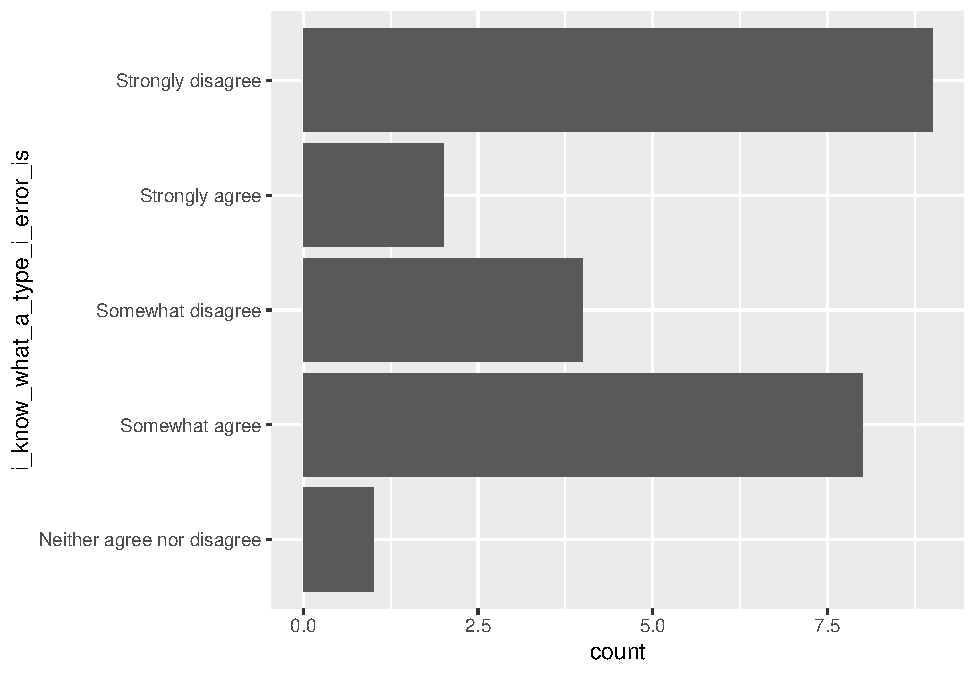
\includegraphics{test_course_notes_files/figure-latex/unnamed-chunk-12-1.pdf}

The second way does this implicitly, using the pipe operator. Note that the results should be the same.

\begin{Shaded}
\begin{Highlighting}[]
\NormalTok{prior\_survey }\SpecialCharTok{\%\textgreater{}\%} 
  \FunctionTok{ggplot}\NormalTok{(}\AttributeTok{mapping =} \FunctionTok{aes}\NormalTok{(}\AttributeTok{x =}\NormalTok{ i\_know\_what\_a\_type\_i\_error\_is)) }\SpecialCharTok{+}
  \FunctionTok{geom\_bar}\NormalTok{() }\SpecialCharTok{+}
  \FunctionTok{coord\_flip}\NormalTok{()}
\end{Highlighting}
\end{Shaded}

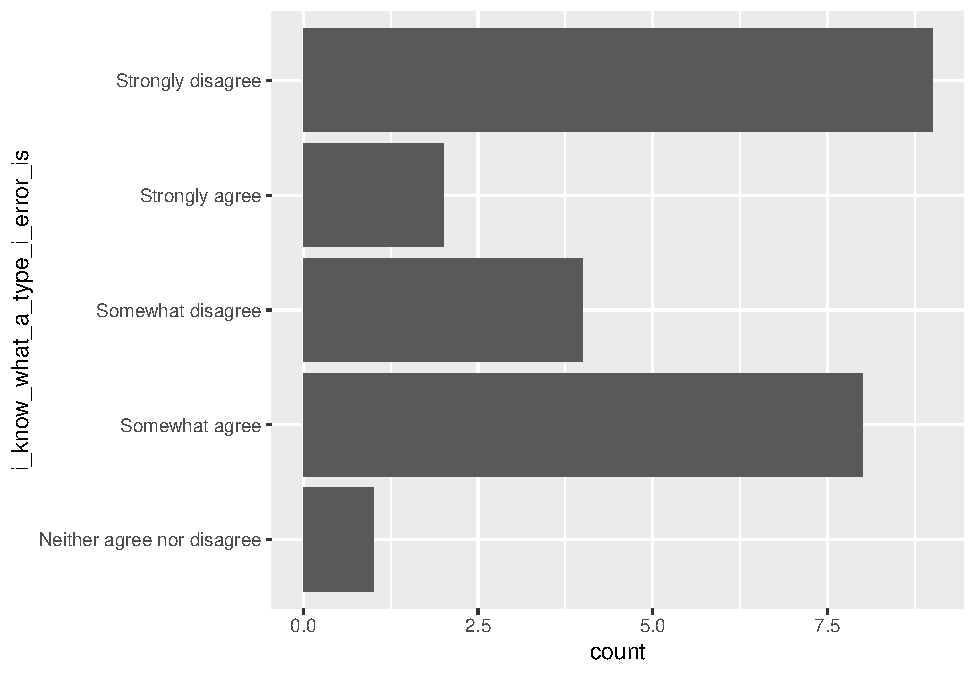
\includegraphics{test_course_notes_files/figure-latex/unnamed-chunk-13-1.pdf}

If we wanted to get extra fancy, we could first convert the data from a wide format to a long format and then start plotting all the items together.

Converting to long format would produce something like this:

\begin{Shaded}
\begin{Highlighting}[]
\NormalTok{prior\_survey }\SpecialCharTok{\%\textgreater{}\%} 
  \FunctionTok{gather}\NormalTok{(}\AttributeTok{key =} \StringTok{"survey\_item"}\NormalTok{, }\AttributeTok{value =} \StringTok{"survey\_response"}\NormalTok{)}
\end{Highlighting}
\end{Shaded}

\begin{verbatim}
## # A tibble: 1,176 x 2
##    survey_item survey_response
##    <chr>       <chr>          
##  1 student_id  1              
##  2 student_id  2              
##  3 student_id  3              
##  4 student_id  4              
##  5 student_id  5              
##  6 student_id  6              
##  7 student_id  7              
##  8 student_id  8              
##  9 student_id  9              
## 10 student_id  10             
## # ... with 1,166 more rows
\end{verbatim}

Then we can combine that with the \texttt{group\_by()} and \texttt{summarize()} functions and plot the results.

\begin{Shaded}
\begin{Highlighting}[]
\NormalTok{prior\_survey }\SpecialCharTok{\%\textgreater{}\%} 
  \FunctionTok{gather}\NormalTok{(}\AttributeTok{key =} \StringTok{"survey\_item"}\NormalTok{, }\AttributeTok{value =} \StringTok{"survey\_response"}\NormalTok{) }\SpecialCharTok{\%\textgreater{}\%} 
  \FunctionTok{group\_by}\NormalTok{(survey\_item, survey\_response) }\SpecialCharTok{\%\textgreater{}\%} 
  \FunctionTok{summarize}\NormalTok{(}\AttributeTok{n =} \FunctionTok{n}\NormalTok{()) }\SpecialCharTok{\%\textgreater{}\%} 
  \FunctionTok{ggplot}\NormalTok{(}\AttributeTok{mapping =} \FunctionTok{aes}\NormalTok{(}\AttributeTok{x =}\NormalTok{ survey\_response, }\AttributeTok{y =}\NormalTok{ survey\_item, }\AttributeTok{fill =}\NormalTok{ n)) }\SpecialCharTok{+}
  \FunctionTok{geom\_tile}\NormalTok{()}
\end{Highlighting}
\end{Shaded}

\begin{verbatim}
## `summarise()` regrouping output by 'survey_item' (override with `.groups` argument)
\end{verbatim}

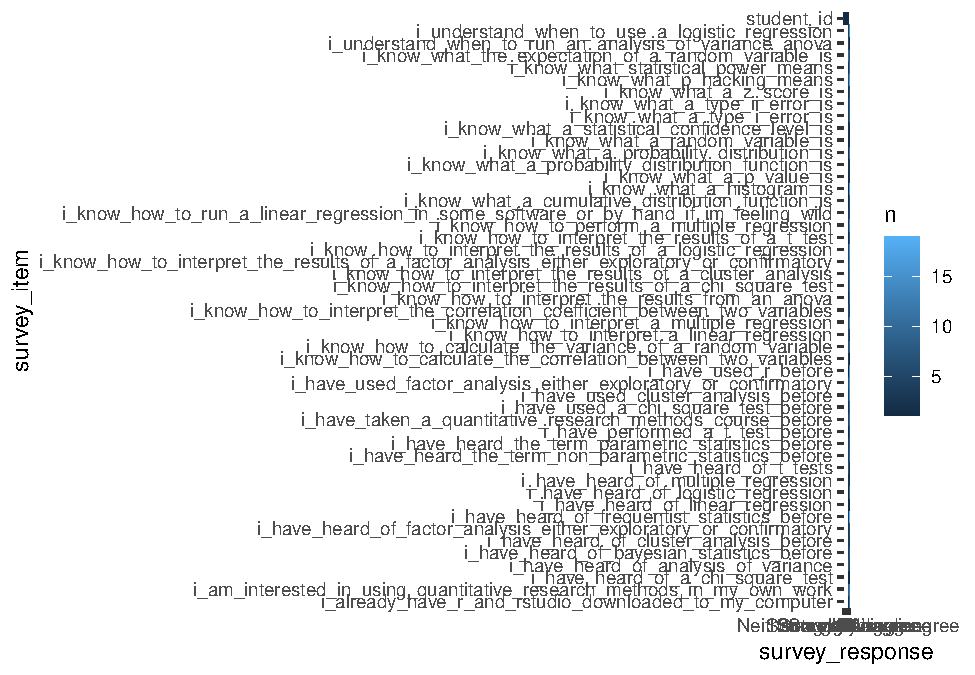
\includegraphics{test_course_notes_files/figure-latex/unnamed-chunk-15-1.pdf}

This plot is okay for giving a general sense of what is going on in these plots but there are a bunch of other ways to go about doing this.

First, maybe we want to rename the response categories to a numerical scale. We can accomplish this with a \texttt{mutate()} and \texttt{case\_when()}.

\begin{Shaded}
\begin{Highlighting}[]
\NormalTok{prior\_survey }\OtherTok{\textless{}{-}}\NormalTok{ prior\_survey }\SpecialCharTok{\%\textgreater{}\%} 
  \FunctionTok{gather}\NormalTok{(}\AttributeTok{key =} \StringTok{"survey\_item"}\NormalTok{, }\AttributeTok{value =} \StringTok{"survey\_response"}\NormalTok{) }\SpecialCharTok{\%\textgreater{}\%} 
  \FunctionTok{mutate}\NormalTok{(}\AttributeTok{survey\_response\_num =} \FunctionTok{case\_when}\NormalTok{(survey\_response }\SpecialCharTok{==} \StringTok{"Strongly disagree"} \SpecialCharTok{\textasciitilde{}} \DecValTok{0}\NormalTok{,}
\NormalTok{                                         survey\_response }\SpecialCharTok{==} \StringTok{"Somewhat disagree"} \SpecialCharTok{\textasciitilde{}} \DecValTok{1}\NormalTok{,}
\NormalTok{                                         survey\_response }\SpecialCharTok{==} \StringTok{"Neither agree nor disagree"} \SpecialCharTok{\textasciitilde{}} \DecValTok{2}\NormalTok{,}
\NormalTok{                                         survey\_response }\SpecialCharTok{==} \StringTok{"Somewhat agree"} \SpecialCharTok{\textasciitilde{}} \DecValTok{3}\NormalTok{,}
\NormalTok{                                         survey\_response }\SpecialCharTok{==} \StringTok{"Strongly agree"} \SpecialCharTok{\textasciitilde{}} \DecValTok{4}\NormalTok{,}
\NormalTok{                                         )) }
\end{Highlighting}
\end{Shaded}

Then we plot the same data but with the numerical scale along the x-axis.

\begin{Shaded}
\begin{Highlighting}[]
\NormalTok{prior\_survey }\SpecialCharTok{\%\textgreater{}\%} 
  \FunctionTok{group\_by}\NormalTok{(survey\_item, survey\_response\_num) }\SpecialCharTok{\%\textgreater{}\%} 
  \FunctionTok{summarize}\NormalTok{(}\AttributeTok{n =} \FunctionTok{n}\NormalTok{()) }\SpecialCharTok{\%\textgreater{}\%} 
  \FunctionTok{ggplot}\NormalTok{(}\AttributeTok{mapping =} \FunctionTok{aes}\NormalTok{(}\AttributeTok{x =}\NormalTok{ survey\_response\_num, }\AttributeTok{y =}\NormalTok{ survey\_item, }\AttributeTok{fill =}\NormalTok{ n)) }\SpecialCharTok{+}
  \FunctionTok{geom\_tile}\NormalTok{()}
\end{Highlighting}
\end{Shaded}

\begin{verbatim}
## `summarise()` regrouping output by 'survey_item' (override with `.groups` argument)
\end{verbatim}

\begin{verbatim}
## Warning: Removed 3 rows containing missing values (geom_tile).
\end{verbatim}

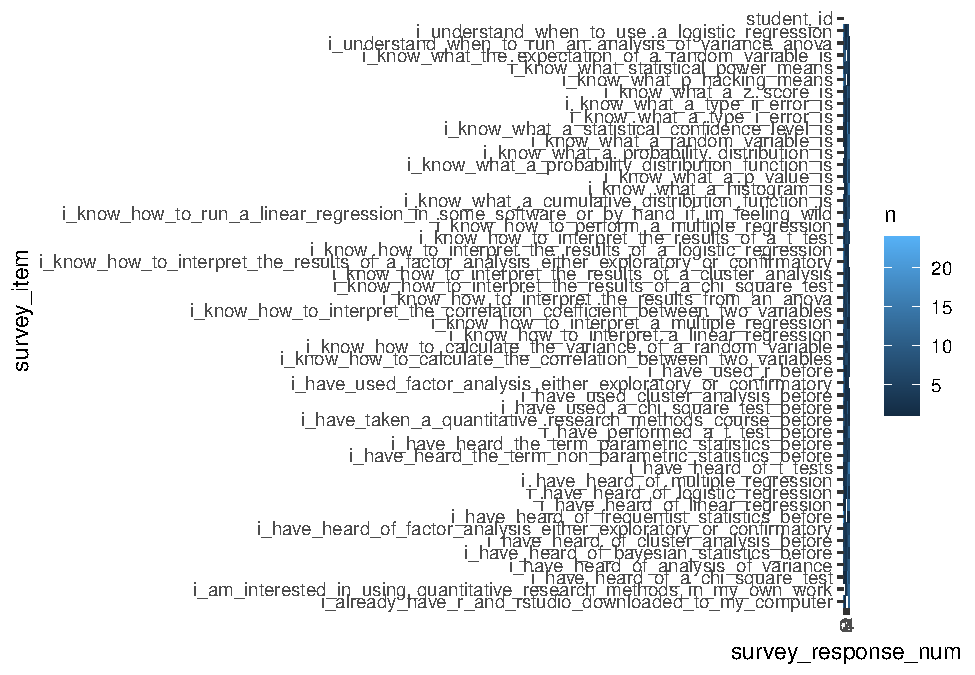
\includegraphics{test_course_notes_files/figure-latex/unnamed-chunk-17-1.pdf}

\hypertarget{some-brief-stats}{%
\section{Some brief stats}\label{some-brief-stats}}

In this week's reading, there was also discussion about standard errors and the central limit theorem. These are fairly important theoretical concepts to grasp. To some extent they deal with the scenario where you go out and repeatedly sample from a population and calculate a statistic from each of those samples. The distributions \emph{of that statistic} is what we will call the sampling distribution (as opposed to the sample distribution, which would more accurately describe the distribution of the data that we get in any one sample that we draw from the population).

\hypertarget{central-limit-theorem-and-standard-error-demo--}{%
\subsection{Central Limit Theorem and Standard Error Demo ----}\label{central-limit-theorem-and-standard-error-demo--}}

\begin{Shaded}
\begin{Highlighting}[]
\NormalTok{pop\_students }\OtherTok{\textless{}{-}} \DecValTok{10000}

\NormalTok{zoom\_min\_pop }\OtherTok{\textless{}{-}} \FunctionTok{rnorm}\NormalTok{(}\AttributeTok{n =}\NormalTok{ pop\_students, }\AttributeTok{mean =} \DecValTok{600}\NormalTok{, }\AttributeTok{sd =} \DecValTok{100}\NormalTok{)}

\FunctionTok{hist}\NormalTok{(zoom\_min\_pop)}
\end{Highlighting}
\end{Shaded}

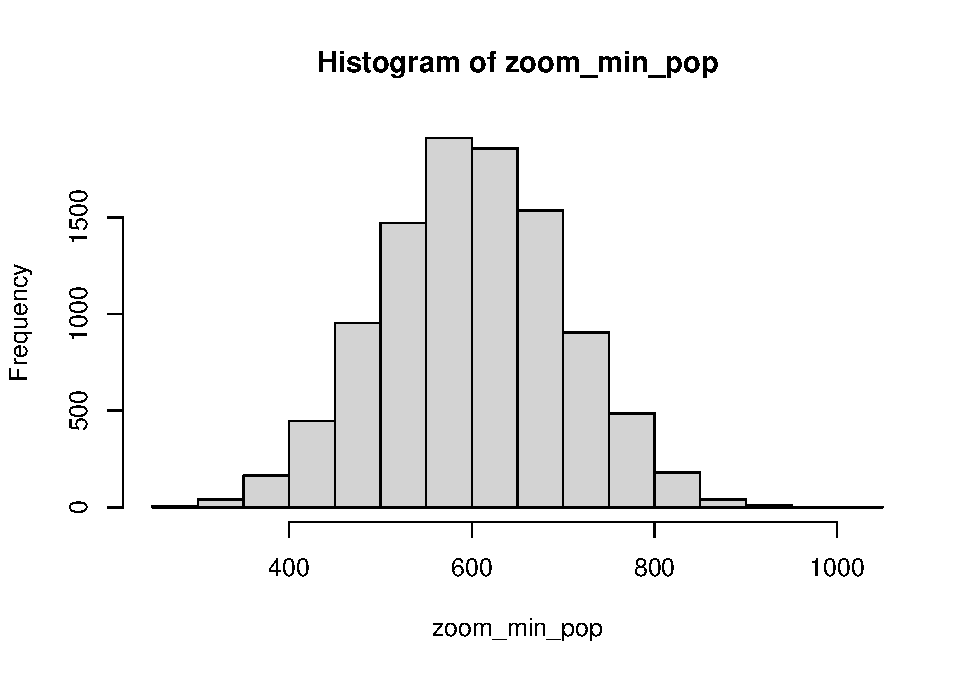
\includegraphics{test_course_notes_files/figure-latex/unnamed-chunk-18-1.pdf}

\begin{Shaded}
\begin{Highlighting}[]
\NormalTok{zoom\_min\_sample }\OtherTok{\textless{}{-}} \FunctionTok{sample}\NormalTok{(}\AttributeTok{x =}\NormalTok{ zoom\_min\_pop,}
                          \AttributeTok{size =} \DecValTok{200}\NormalTok{,}
                          \AttributeTok{replace =} \ConstantTok{FALSE}\NormalTok{)}


\FunctionTok{hist}\NormalTok{(zoom\_min\_sample)}
\end{Highlighting}
\end{Shaded}

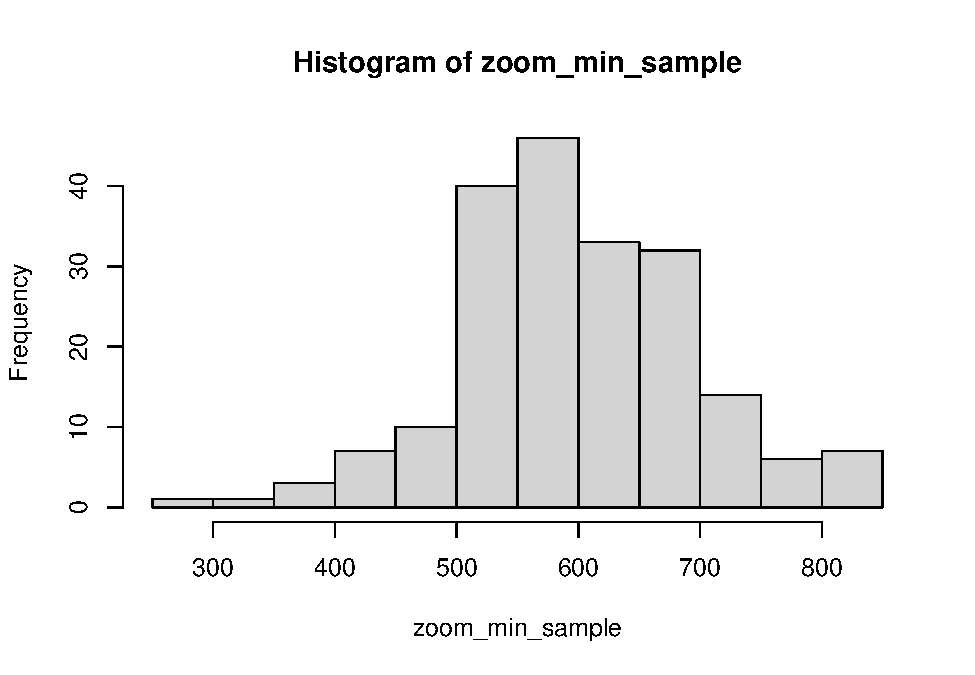
\includegraphics{test_course_notes_files/figure-latex/unnamed-chunk-18-2.pdf}

\begin{Shaded}
\begin{Highlighting}[]
\FunctionTok{mean}\NormalTok{(zoom\_min\_sample)}
\end{Highlighting}
\end{Shaded}

\begin{verbatim}
## [1] 599.5327
\end{verbatim}

\begin{Shaded}
\begin{Highlighting}[]
\FunctionTok{sd}\NormalTok{(zoom\_min\_sample)}
\end{Highlighting}
\end{Shaded}

\begin{verbatim}
## [1] 97.4902
\end{verbatim}

As a brief aside, let's review the idea of a loop

\begin{Shaded}
\begin{Highlighting}[]
\NormalTok{num\_reps }\OtherTok{\textless{}{-}} \DecValTok{100}

\NormalTok{data\_vec }\OtherTok{\textless{}{-}} \FunctionTok{rep}\NormalTok{(}\ConstantTok{NA}\NormalTok{, num\_reps) }\CommentTok{\# this creates an empty vector of size num\_reps with NA in each entry}

\CommentTok{\# this loops through the vector starting at position 1 and ending at the final position (num\_reps). For demonstration purposes, we replacing the NA in each entry with the number of that entry (i.e., the NA in the 20th entry is replaced with the number 20)}

\ControlFlowTok{for}\NormalTok{ (i }\ControlFlowTok{in} \DecValTok{1}\SpecialCharTok{:}\NormalTok{num\_reps)\{}
\NormalTok{  data\_vec[i] }\OtherTok{\textless{}{-}}\NormalTok{ i}
\NormalTok{\}}
\end{Highlighting}
\end{Shaded}

Okay, so that's how we create an empty vector and how we loop through its different entries. For this demo, we will also need to remenber how to generate random numbers from a norm distribution with a specified mean and standard deviation.

\begin{Shaded}
\begin{Highlighting}[]
\FunctionTok{rnorm}\NormalTok{(}\AttributeTok{n =} \DecValTok{10}\NormalTok{, }\AttributeTok{mean =} \DecValTok{5}\NormalTok{, }\AttributeTok{sd =} \DecValTok{2}\NormalTok{) }\CommentTok{\# n is the number of random numbers we draw from this normal distribution}
\end{Highlighting}
\end{Shaded}

\begin{verbatim}
##  [1] 5.373227 6.898946 4.869013 4.753062 3.748130 6.593905 3.719262 5.720239
##  [9] 5.108144 3.017232
\end{verbatim}

Okay, so that's not bad. Now, that command will produce a vector with 10 random numbers. We can calculate the mean and standard deviation of those 10 numbers (which should be close to the values that we specified in \texttt{rnorm()} with the \texttt{mean()} and \texttt{sd()} functions.

\begin{Shaded}
\begin{Highlighting}[]
\FunctionTok{mean}\NormalTok{(}\FunctionTok{rnorm}\NormalTok{(}\AttributeTok{n =} \DecValTok{10}\NormalTok{, }\AttributeTok{mean =} \DecValTok{5}\NormalTok{, }\AttributeTok{sd =} \DecValTok{2}\NormalTok{))}
\end{Highlighting}
\end{Shaded}

\begin{verbatim}
## [1] 5.155702
\end{verbatim}

\begin{Shaded}
\begin{Highlighting}[]
\FunctionTok{sd}\NormalTok{(}\FunctionTok{rnorm}\NormalTok{(}\AttributeTok{n =} \DecValTok{10}\NormalTok{, }\AttributeTok{mean =} \DecValTok{5}\NormalTok{, }\AttributeTok{sd =} \DecValTok{2}\NormalTok{))}
\end{Highlighting}
\end{Shaded}

\begin{verbatim}
## [1] 2.551694
\end{verbatim}

Next, let's act as if we are drawing a certain sample of size \texttt{samp\_size} of data points for \texttt{num\_reps} number of times. Keep in mind that, in practice, when we are collecting data ourselves in our own research, num\_reps will almost always be 1. We are just demonstrating the underlying assumptions for how we can calculate some of the statistics that we use.

\begin{Shaded}
\begin{Highlighting}[]
\NormalTok{num\_reps }\OtherTok{\textless{}{-}} \DecValTok{1000} \CommentTok{\# specify how many times to take a sample}
\NormalTok{samp\_size }\OtherTok{\textless{}{-}} \DecValTok{200} \CommentTok{\# specify the size of each sample}
\NormalTok{data\_vec }\OtherTok{\textless{}{-}} \FunctionTok{rep}\NormalTok{(}\ConstantTok{NA}\NormalTok{, num\_reps) }\CommentTok{\# create an empty vector of size num\_reps with NA in each entry.}
\ControlFlowTok{for}\NormalTok{ (i }\ControlFlowTok{in} \DecValTok{1}\SpecialCharTok{:}\NormalTok{num\_reps)\{}
\NormalTok{  data\_vec[i] }\OtherTok{\textless{}{-}} \FunctionTok{mean}\NormalTok{(}\FunctionTok{rnorm}\NormalTok{(}\AttributeTok{n =}\NormalTok{ samp\_size, }\AttributeTok{mean =} \DecValTok{600}\NormalTok{, }\AttributeTok{sd =} \DecValTok{100}\NormalTok{)) }\CommentTok{\# store the mean of each of the num\_rep samples}
\NormalTok{\}}
\end{Highlighting}
\end{Shaded}

With this, we have a vector \texttt{data\_vec} of size \texttt{num\_reps} with the mean of each of our samples that we drew. This vector contains our sampling distribution of our sample means. \textbf{NOTE}: The standard deviation of this sampling mean is what we are calling our \emph{standard error}.

We can plot a histogram of this sampling distribution and calculate the standard deviation of the sampling mean.

\begin{Shaded}
\begin{Highlighting}[]
\FunctionTok{hist}\NormalTok{(data\_vec)}
\end{Highlighting}
\end{Shaded}

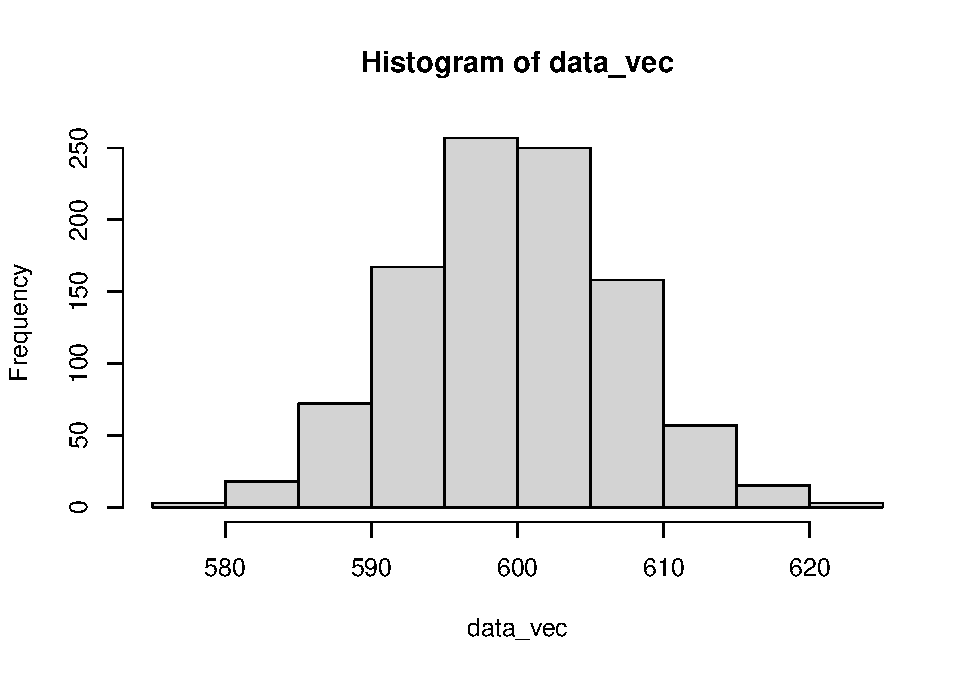
\includegraphics{test_course_notes_files/figure-latex/unnamed-chunk-23-1.pdf}

\begin{Shaded}
\begin{Highlighting}[]
\FunctionTok{sd}\NormalTok{(data\_vec)}
\end{Highlighting}
\end{Shaded}

\begin{verbatim}
## [1] 7.171118
\end{verbatim}

On your own, try copying this code and changing the num\_reps and sample\_size variables to larger and smaller values. Focus on how the x-axis values in your histogram change when you change the num\_reps and samp\_size variables.

Hint: CLT will explain the normal distribution of the sampling mean (the shape you see in the histogram) while the Weak Law of Large Numbers will explain the concentration around the true mean as samp\_size increases (i.e., when we draw a larger sample size from the population, our sample mean gets closer to the population mean).

\begin{Shaded}
\begin{Highlighting}[]
\DocumentationTok{\#\# Quick note on the rep() function: notice what happens when you specify "each" vs "times".}
\FunctionTok{rep}\NormalTok{(}\FunctionTok{c}\NormalTok{(}\DecValTok{1}\NormalTok{, }\DecValTok{2}\NormalTok{), }\AttributeTok{times =} \DecValTok{5}\NormalTok{)}
\end{Highlighting}
\end{Shaded}

\begin{verbatim}
##  [1] 1 2 1 2 1 2 1 2 1 2
\end{verbatim}

\begin{Shaded}
\begin{Highlighting}[]
\FunctionTok{rep}\NormalTok{(}\FunctionTok{c}\NormalTok{(}\DecValTok{1}\NormalTok{, }\DecValTok{2}\NormalTok{), }\AttributeTok{each =} \DecValTok{5}\NormalTok{)}
\end{Highlighting}
\end{Shaded}

\begin{verbatim}
##  [1] 1 1 1 1 1 2 2 2 2 2
\end{verbatim}

\hypertarget{week-3-data-cleaning-organizing-describing-and-communicating}{%
\chapter{Week 3: Data Cleaning, Organizing, Describing, and Communicating}\label{week-3-data-cleaning-organizing-describing-and-communicating}}

This week we focus on different steps you will often take when you first start working with your data. These tend to fall under the umbrella of ``data processing'' and often need to happen before you can start doing any kind of analysis.

\hypertarget{visualizing-your-data}{%
\section{Visualizing your data}\label{visualizing-your-data}}

Once your data have been clearned, you are ready to start visualizing what you are working with. There is a huge range of what you can do with these plots. That's great! On the other hand, it can quickly start to feel overwhelming. To help get this under control and make it more manageable, it is convenient to think about the \emph{types} of data that you have. In particular, are your variables nominal, ordinal, interval, or ratio variables?

\hypertarget{one-continuous-variable-either-predictor-or-outcome-variable}{%
\subsection{One continuous variable (either predictor or outcome variable)}\label{one-continuous-variable-either-predictor-or-outcome-variable}}

When you have one continuous variable, a standard option is to plot a histogram. These are plots that show the frequency of each of the values that the variable takes. Oftentimes it is helpful to create bins of values so that any number that falls in the 0-4 range counts in one bin, numbers from 5-9 are in a second bin, and so on.

For this example, we will start by generating some data using \texttt{rnorm()}, which generates a random number (or in our case, \texttt{num} numbers) from a normal distribution with mean \texttt{mu} and standard deviation \texttt{stdev}.

\begin{Shaded}
\begin{Highlighting}[]
\NormalTok{num }\OtherTok{\textless{}{-}} \DecValTok{50}
\NormalTok{mu }\OtherTok{\textless{}{-}} \DecValTok{5}
\NormalTok{stdev }\OtherTok{\textless{}{-}} \DecValTok{2}

\NormalTok{x }\OtherTok{\textless{}{-}} \FunctionTok{rnorm}\NormalTok{(}\AttributeTok{n =}\NormalTok{ num, }\AttributeTok{mean =}\NormalTok{ mu, }\AttributeTok{sd =}\NormalTok{ stdev)}
\end{Highlighting}
\end{Shaded}

With these data generated, we can then quickly plot the histogram with \texttt{hist()}. This will use base R graphics.

\begin{Shaded}
\begin{Highlighting}[]
\FunctionTok{hist}\NormalTok{(x)}
\end{Highlighting}
\end{Shaded}

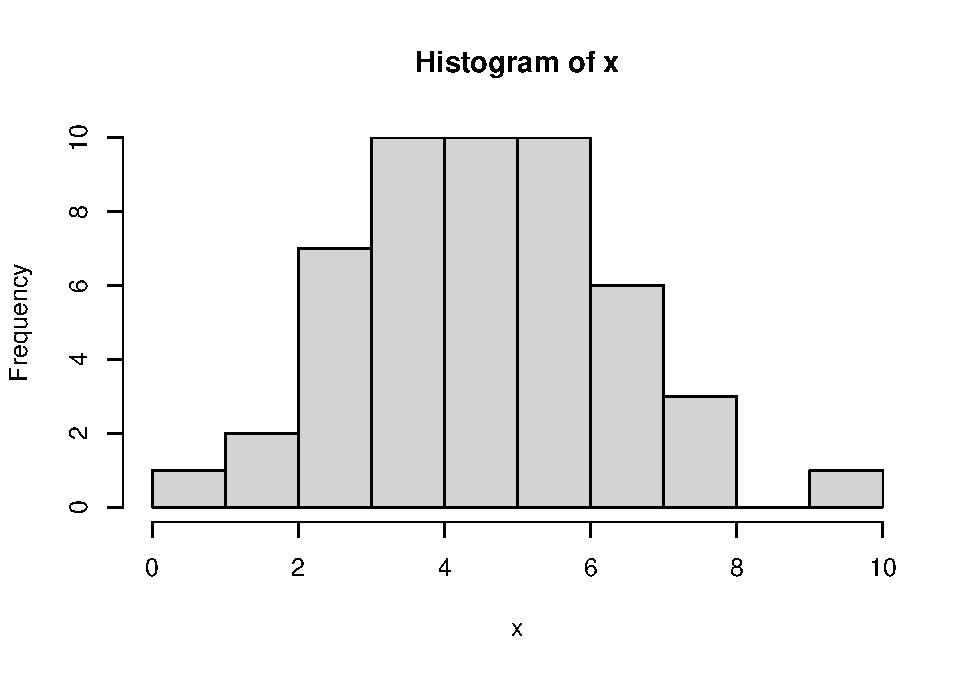
\includegraphics{test_course_notes_files/figure-latex/unnamed-chunk-25-1.pdf}

You can also do this using ggplot rather than base R graphics.

\begin{Shaded}
\begin{Highlighting}[]
\NormalTok{x\_df }\OtherTok{\textless{}{-}} \FunctionTok{tibble}\NormalTok{(}\AttributeTok{x\_col =}\NormalTok{ x)}

\FunctionTok{ggplot}\NormalTok{(}\AttributeTok{data =}\NormalTok{ x\_df, }\AttributeTok{mapping =} \FunctionTok{aes}\NormalTok{(}\AttributeTok{x =}\NormalTok{ x\_col)) }\SpecialCharTok{+}
  \FunctionTok{geom\_histogram}\NormalTok{()}
\end{Highlighting}
\end{Shaded}

\begin{verbatim}
## `stat_bin()` using `bins = 30`. Pick better value with `binwidth`.
\end{verbatim}

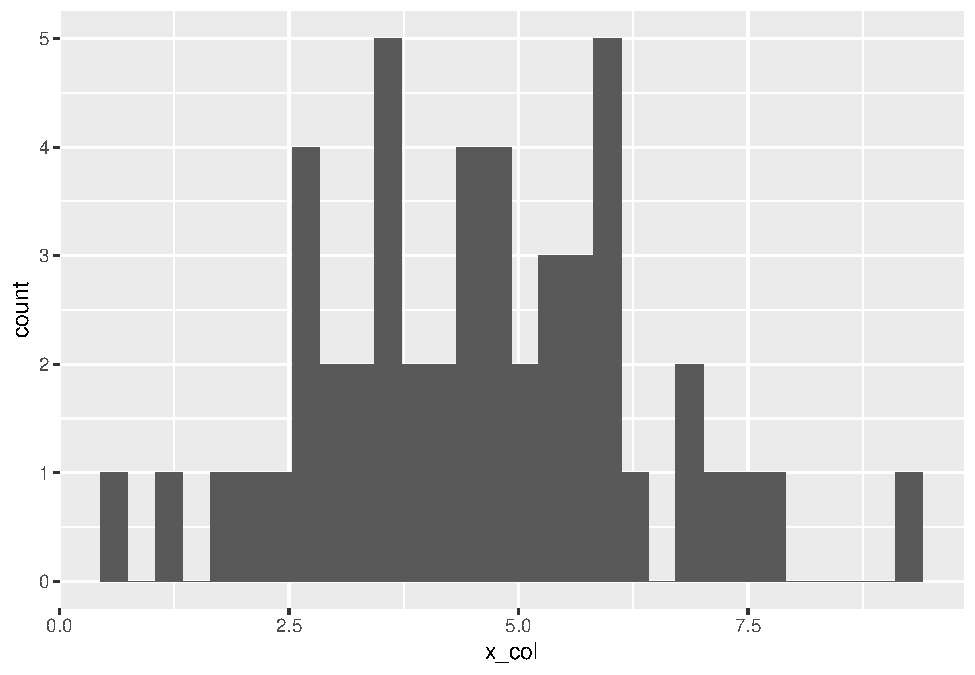
\includegraphics{test_course_notes_files/figure-latex/ggplot-hist-1.pdf}

The histogram is a very standard plot, and you should consider it a go-to option in your toolkit. Alternatively, you can use geom\_density() instead of geom\_histogram() to get a smooth graph rather than one with discrete bins. We will use the same data that we generated before.

We will write this two ways to demnostrate how the pipe \texttt{\%\textgreater{}\%} operator works.

First way:

\begin{Shaded}
\begin{Highlighting}[]
\FunctionTok{ggplot}\NormalTok{(}\AttributeTok{data =}\NormalTok{ x\_df, }\AttributeTok{mapping =} \FunctionTok{aes}\NormalTok{(}\AttributeTok{x =}\NormalTok{ x\_col)) }\SpecialCharTok{+}
  \FunctionTok{geom\_density}\NormalTok{()}
\end{Highlighting}
\end{Shaded}

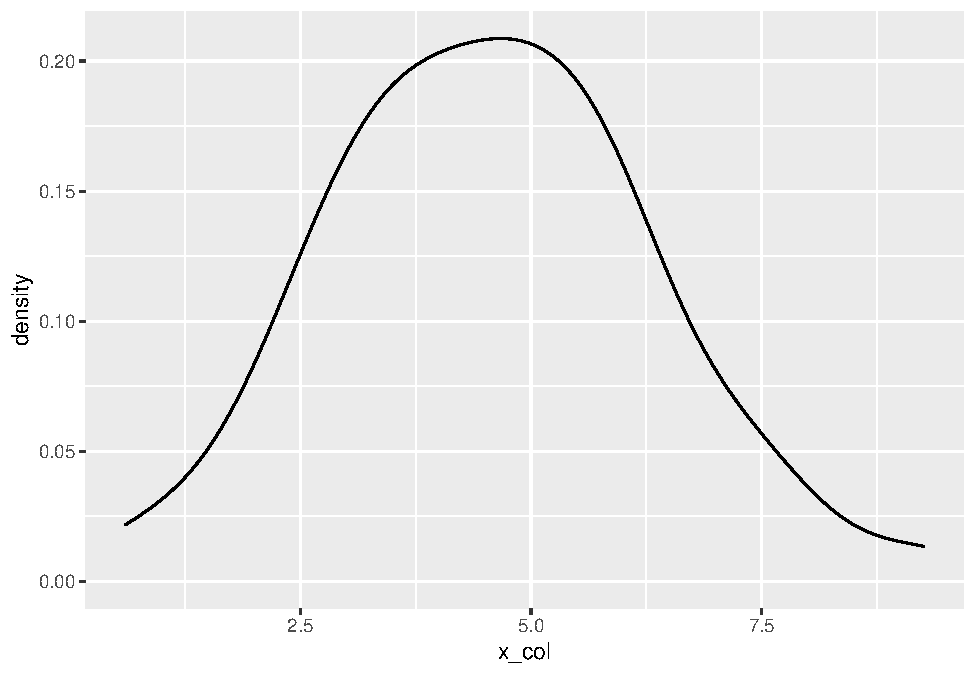
\includegraphics{test_course_notes_files/figure-latex/unnamed-chunk-26-1.pdf}

Second way:

\begin{Shaded}
\begin{Highlighting}[]
\NormalTok{x\_df }\SpecialCharTok{\%\textgreater{}\%}
  \FunctionTok{ggplot}\NormalTok{(}\AttributeTok{mapping =} \FunctionTok{aes}\NormalTok{(}\AttributeTok{x =}\NormalTok{ x\_col)) }\SpecialCharTok{+}
  \FunctionTok{geom\_density}\NormalTok{()}
\end{Highlighting}
\end{Shaded}

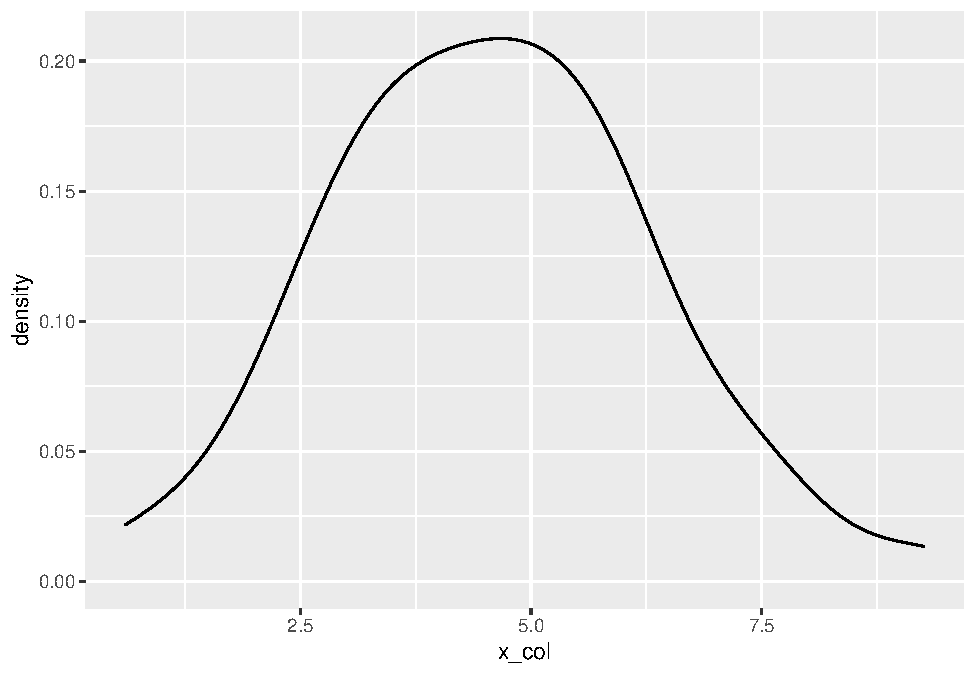
\includegraphics{test_course_notes_files/figure-latex/unnamed-chunk-27-1.pdf}

Just for fun, look at what happens to the the plot if you increase the sample size

First, we will generate the data with a sample size of 5,000 rather than 50.

\begin{Shaded}
\begin{Highlighting}[]
\NormalTok{num }\OtherTok{\textless{}{-}} \DecValTok{5000}
\NormalTok{mu }\OtherTok{\textless{}{-}} \DecValTok{5}
\NormalTok{stdev }\OtherTok{\textless{}{-}} \DecValTok{2}

\NormalTok{x }\OtherTok{\textless{}{-}} \FunctionTok{rnorm}\NormalTok{(}\AttributeTok{n =}\NormalTok{ num, }\AttributeTok{mean =}\NormalTok{ mu, }\AttributeTok{sd =}\NormalTok{ stdev)}
\NormalTok{x\_df }\OtherTok{\textless{}{-}} \FunctionTok{tibble}\NormalTok{(}\AttributeTok{x\_col =}\NormalTok{ x)}
\end{Highlighting}
\end{Shaded}

Then we will plot the histogram

\begin{Shaded}
\begin{Highlighting}[]
\NormalTok{x\_df }\SpecialCharTok{\%\textgreater{}\%} 
  \FunctionTok{ggplot}\NormalTok{(}\FunctionTok{aes}\NormalTok{(}\AttributeTok{x =}\NormalTok{ x\_col)) }\SpecialCharTok{+}
  \FunctionTok{geom\_histogram}\NormalTok{() }\SpecialCharTok{+}
  \FunctionTok{labs}\NormalTok{(}\AttributeTok{x =} \StringTok{"x value"}\NormalTok{,}
       \AttributeTok{y =} \StringTok{"Count"}\NormalTok{,}
       \AttributeTok{title =} \StringTok{"Histogram of normal distribution with n = 5000, mu = 5, sd = 2"}\NormalTok{)}
\end{Highlighting}
\end{Shaded}

\begin{verbatim}
## `stat_bin()` using `bins = 30`. Pick better value with `binwidth`.
\end{verbatim}

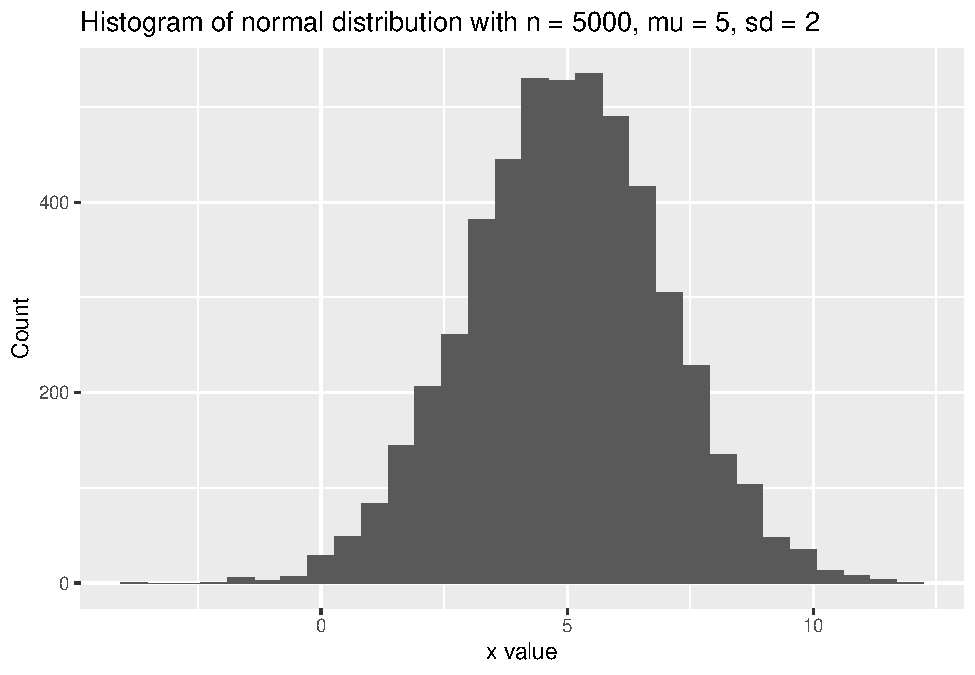
\includegraphics{test_course_notes_files/figure-latex/unnamed-chunk-29-1.pdf}

And, finally, we can make the density plot instead of the histogram, if that's our jam.

\begin{Shaded}
\begin{Highlighting}[]
\FunctionTok{ggplot}\NormalTok{(}\AttributeTok{data =}\NormalTok{ x\_df, }\AttributeTok{mapping =} \FunctionTok{aes}\NormalTok{(}\AttributeTok{x =}\NormalTok{ x\_col)) }\SpecialCharTok{+}
  \FunctionTok{geom\_density}\NormalTok{()}
\end{Highlighting}
\end{Shaded}

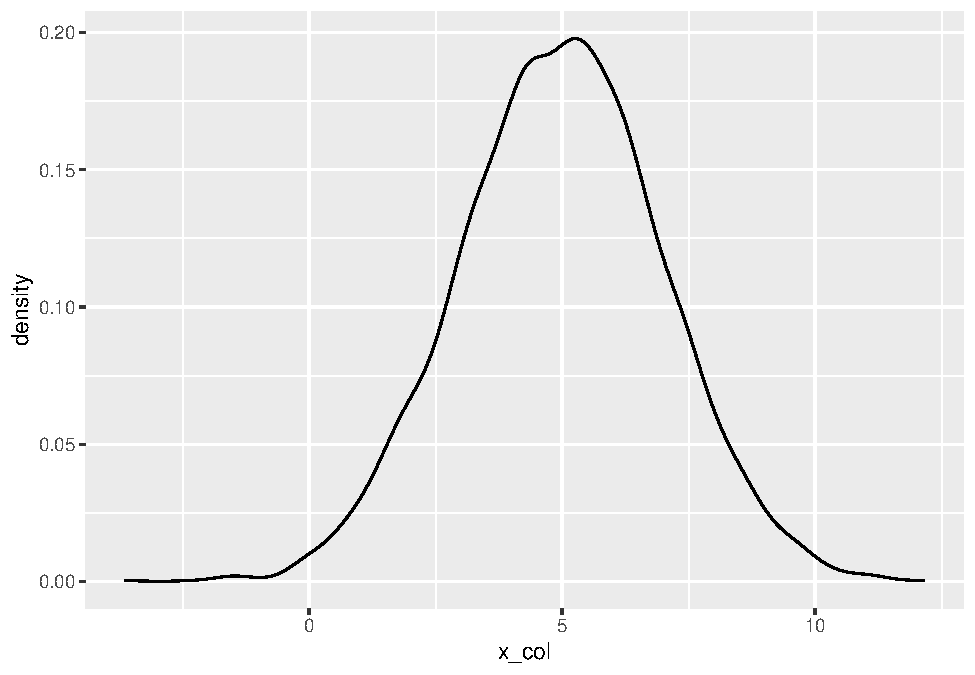
\includegraphics{test_course_notes_files/figure-latex/unnamed-chunk-30-1.pdf}

\hypertarget{one-discrete-variable-either-predictor-or-outcome}{%
\subsection{One Discrete Variable (either predictor or outcome)}\label{one-discrete-variable-either-predictor-or-outcome}}

What if instead of a continuous (i.e., interval or ratio) variable we have a discrete variable such as a nominal (e.g., major, university) or ordinal (e.g., Likert scale item, level of education) variable? For that we can use something like \texttt{geom\_bar()} or \texttt{geom\_col()} to plot the counts of observations within each of those categories.

To demonstrate this, we first need some data to work with. We will use the pre-semester, prior knowledge survey that everyone took. I have combined this year's results with last year's results in order to increase the sample size. After reading in the data, I will also use the \texttt{clean\_names()} function from the \texttt{janitor} package.

\begin{Shaded}
\begin{Highlighting}[]
\DocumentationTok{\#\# load in the data}
\NormalTok{survey\_df }\OtherTok{\textless{}{-}} \FunctionTok{read\_csv}\NormalTok{(}\StringTok{"ENGE\_5714\_2021\_pre\_survey.csv"}\NormalTok{)}
\end{Highlighting}
\end{Shaded}

\begin{verbatim}
## Parsed with column specification:
## cols(
##   .default = col_character(),
##   student_id = col_double()
## )
\end{verbatim}

\begin{verbatim}
## See spec(...) for full column specifications.
\end{verbatim}

\begin{Shaded}
\begin{Highlighting}[]
\NormalTok{survey\_df }\OtherTok{\textless{}{-}}\NormalTok{ survey\_df }\SpecialCharTok{\%\textgreater{}\%} \FunctionTok{clean\_names}\NormalTok{()}
\end{Highlighting}
\end{Shaded}

Next, we can go ahead and make a bar plot with the following code:

\begin{Shaded}
\begin{Highlighting}[]
\NormalTok{survey\_df }\SpecialCharTok{\%\textgreater{}\%} 
  \FunctionTok{ggplot}\NormalTok{(}\FunctionTok{aes}\NormalTok{(}\AttributeTok{x =}\NormalTok{ i\_have\_taken\_a\_quantitative\_research\_methods\_course\_before)) }\SpecialCharTok{+}
  \FunctionTok{geom\_bar}\NormalTok{()}
\end{Highlighting}
\end{Shaded}

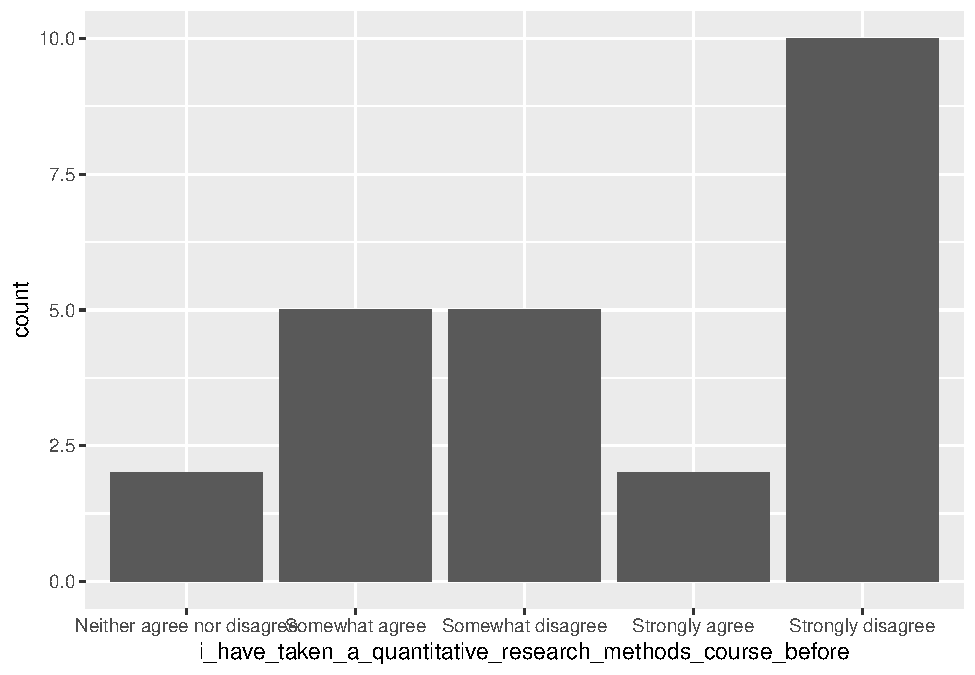
\includegraphics{test_course_notes_files/figure-latex/geom-bar-1.pdf}

Notice that the ordering is not quite what we would want. It is alphabetical. Let's try to fix this.

Here is one way: we first specify the levels of that variable (i.e., the different values that it could take) and store that in the variable \texttt{q\_levels}. Then, we pass that to the \texttt{factor()} function, which will tell R that we want whichever variable is passed to \texttt{factor()} two things. First, it will say that we want to make that variable a factor variable with \texttt{levels\ =\ ...}. Second, we set \texttt{ordered\ =\ TRUE} to tell R that there is a specific ordering to that variable. This way, whenever there is something like a plot that we make, the ordering will persist in the labeling and R will not show the labels in alphabetical order.

Here is an example of that in action:

\begin{Shaded}
\begin{Highlighting}[]
\NormalTok{q\_levels }\OtherTok{\textless{}{-}} \FunctionTok{c}\NormalTok{(}\StringTok{"Strongly disagree"}\NormalTok{, }\StringTok{"Somewhat disagree"}\NormalTok{, }\StringTok{"Neither agree nor disagree"}\NormalTok{,}
              \StringTok{"Somewhat agree"}\NormalTok{, }\StringTok{"Strongly agree"}\NormalTok{)}



\NormalTok{survey\_df}\SpecialCharTok{$}\NormalTok{i\_have\_taken\_a\_quantitative\_research\_methods\_course\_before }\OtherTok{\textless{}{-}} \FunctionTok{factor}\NormalTok{(survey\_df}\SpecialCharTok{$}\NormalTok{i\_have\_taken\_a\_quantitative\_research\_methods\_course\_before, }
                                                                               \AttributeTok{levels =}\NormalTok{ q\_levels,}
                                                                               \AttributeTok{ordered =} \ConstantTok{TRUE}\NormalTok{)}
\end{Highlighting}
\end{Shaded}

Now try plotting these data. We will also add in a \texttt{coord\_flip()} to plot the categories along the y-axis. This is a common move to avoid text from the different levels overlapping with each other. Finally, we will also change the x, y, and title labels with \texttt{labs()}.

\begin{Shaded}
\begin{Highlighting}[]
\NormalTok{survey\_df }\SpecialCharTok{\%\textgreater{}\%} 
  \FunctionTok{ggplot}\NormalTok{(}\FunctionTok{aes}\NormalTok{(}\AttributeTok{x =}\NormalTok{ i\_have\_taken\_a\_quantitative\_research\_methods\_course\_before)) }\SpecialCharTok{+}
  \FunctionTok{geom\_bar}\NormalTok{() }\SpecialCharTok{+}
  \FunctionTok{coord\_flip}\NormalTok{() }\SpecialCharTok{+}
  \FunctionTok{labs}\NormalTok{(}\AttributeTok{x =} \StringTok{"I have taken a quantitative research methods course before"}\NormalTok{,}
       \AttributeTok{y =} \StringTok{"Count"}\NormalTok{,}
       \AttributeTok{title =} \StringTok{"Reordered Example"}\NormalTok{)}
\end{Highlighting}
\end{Shaded}

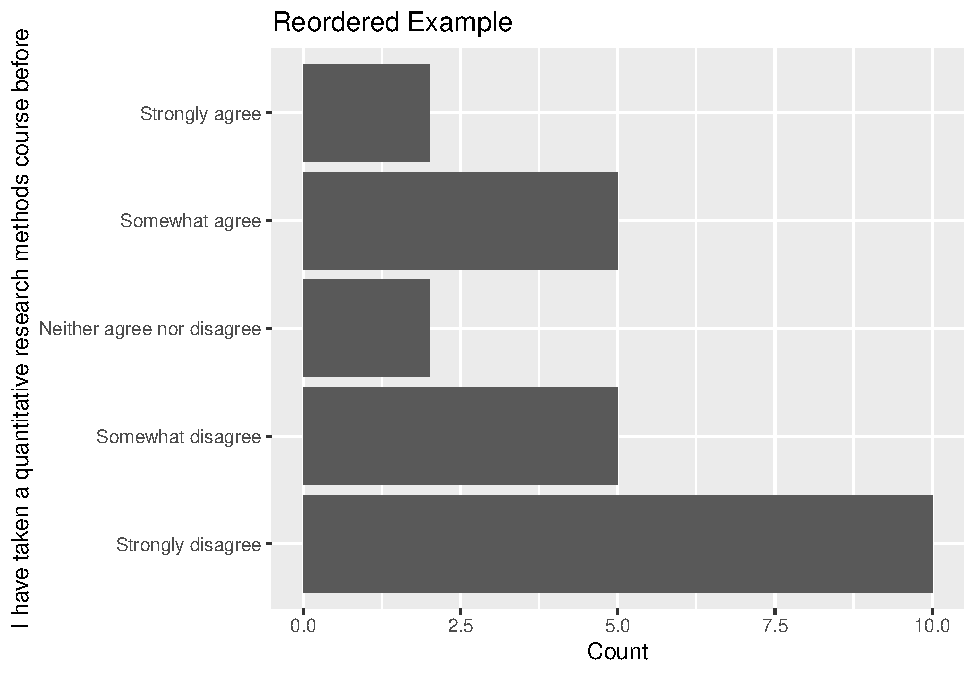
\includegraphics{test_course_notes_files/figure-latex/unnamed-chunk-32-1.pdf}

\hypertarget{joining-two-datasets}{%
\section{Joining two datasets}\label{joining-two-datasets}}

Let's imagine that we have a separate dataset that has information about the students who completed the pre-course prior knowledge survey.

First, we will load in that dataset

\begin{Shaded}
\begin{Highlighting}[]
\NormalTok{survey\_info\_df }\OtherTok{\textless{}{-}} \FunctionTok{read\_csv}\NormalTok{(}\StringTok{"survey\_student\_info.csv"}\NormalTok{)}
\end{Highlighting}
\end{Shaded}

\begin{verbatim}
## Parsed with column specification:
## cols(
##   student_id = col_double(),
##   standing = col_character(),
##   college = col_character(),
##   required = col_character()
## )
\end{verbatim}

Next, let's join the two datasets based on the student id column, which is in each of the two dataframes.

\begin{Shaded}
\begin{Highlighting}[]
\NormalTok{survey\_df }\OtherTok{\textless{}{-}}\NormalTok{ survey\_df }\SpecialCharTok{\%\textgreater{}\%} \FunctionTok{inner\_join}\NormalTok{(survey\_info\_df, }\AttributeTok{by =} \StringTok{"student\_id"}\NormalTok{)}
\end{Highlighting}
\end{Shaded}

Now we should have both datasets joined into one and saved as survey\_df.

With this, we can make some nicer plots and do something like use facet\_grid() to look at students who are masters and doctoral students, for example.

\begin{Shaded}
\begin{Highlighting}[]
\NormalTok{survey\_df }\SpecialCharTok{\%\textgreater{}\%} 
  \FunctionTok{ggplot}\NormalTok{(}\FunctionTok{aes}\NormalTok{(}\AttributeTok{x =}\NormalTok{ i\_have\_taken\_a\_quantitative\_research\_methods\_course\_before)) }\SpecialCharTok{+}
  \FunctionTok{geom\_bar}\NormalTok{() }\SpecialCharTok{+}
  \FunctionTok{facet\_grid}\NormalTok{(standing }\SpecialCharTok{\textasciitilde{}}\NormalTok{.) }\SpecialCharTok{+}
  \FunctionTok{labs}\NormalTok{(}\AttributeTok{x =} \StringTok{"I have taken a quantitative research methods course before"}\NormalTok{,}
       \AttributeTok{y =} \StringTok{"Count"}\NormalTok{,}
       \AttributeTok{title =} \StringTok{"Reordered Example"}\NormalTok{)}
\end{Highlighting}
\end{Shaded}

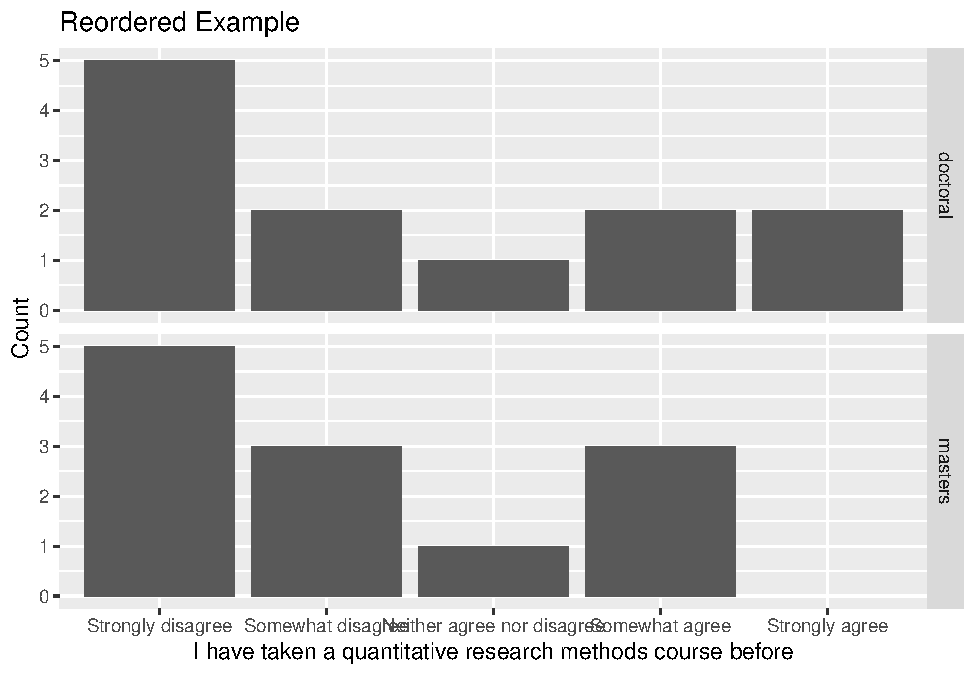
\includegraphics{test_course_notes_files/figure-latex/unnamed-chunk-35-1.pdf}

The x axis looks a little crowded. What if we try \texttt{coord\_flip()}?

\begin{Shaded}
\begin{Highlighting}[]
\NormalTok{survey\_df }\SpecialCharTok{\%\textgreater{}\%} 
  \FunctionTok{filter}\NormalTok{(standing }\SpecialCharTok{==} \StringTok{"doctoral"}\NormalTok{) }\SpecialCharTok{\%\textgreater{}\%}
  \FunctionTok{ggplot}\NormalTok{(}\FunctionTok{aes}\NormalTok{(}\AttributeTok{x =}\NormalTok{ i\_have\_taken\_a\_quantitative\_research\_methods\_course\_before)) }\SpecialCharTok{+}
  \FunctionTok{geom\_bar}\NormalTok{() }\SpecialCharTok{+}
  \FunctionTok{coord\_flip}\NormalTok{() }\SpecialCharTok{+}
  \FunctionTok{facet\_grid}\NormalTok{(standing }\SpecialCharTok{\textasciitilde{}}\NormalTok{.) }\SpecialCharTok{+}
  \FunctionTok{labs}\NormalTok{(}\AttributeTok{x =} \StringTok{"I have taken a quantitative research methods course before"}\NormalTok{,}
       \AttributeTok{y =} \StringTok{"Count"}\NormalTok{,}
       \AttributeTok{title =} \StringTok{"Reordered Example"}\NormalTok{)}
\end{Highlighting}
\end{Shaded}

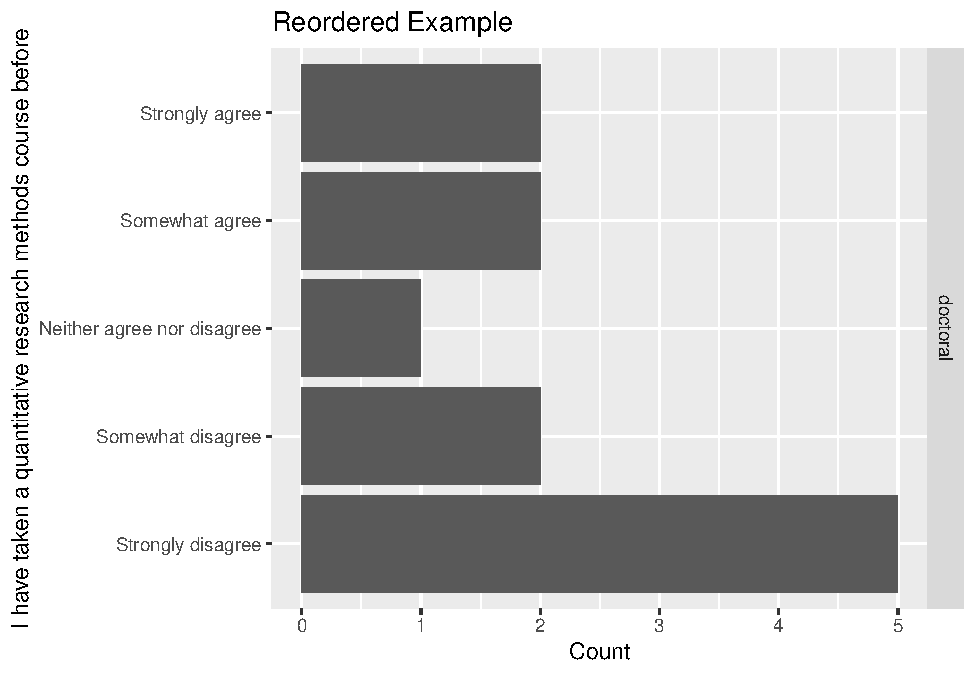
\includegraphics{test_course_notes_files/figure-latex/unnamed-chunk-36-1.pdf}

That looks much better.

\hypertarget{a-quick-note-on-filters}{%
\subsubsection*{A quick note on filters}\label{a-quick-note-on-filters}}
\addcontentsline{toc}{subsubsection}{A quick note on filters}

If you want to look at only a subset of your data, you will want to use the \texttt{filter()} function. The general idea is that you can look at observations (rows) that match a certain criteria. For example, you may want to only look at students from a certain region or year or major. In our case, with the prior knowledge survey, let's say we only want to look at student who have to take the course (i.e., there is a ``yes'' for them for the \texttt{required} variable). We can do that with the first line. The second line just stores the result as a new dataframe called \texttt{filtered\_df}.

\begin{Shaded}
\begin{Highlighting}[]
\NormalTok{survey\_df }\SpecialCharTok{\%\textgreater{}\%} \FunctionTok{filter}\NormalTok{(required }\SpecialCharTok{==} \StringTok{"yes"}\NormalTok{)}
\end{Highlighting}
\end{Shaded}

\begin{verbatim}
## # A tibble: 12 x 52
##    student_id i_have_taken_a_~ i_am_interested~ i_know_what_a_t~
##         <dbl> <ord>            <chr>            <chr>           
##  1          1 Somewhat disagr~ Somewhat agree   Strongly disagr~
##  2          2 Strongly disagr~ Neither agree n~ Somewhat agree  
##  3          4 Somewhat disagr~ Strongly agree   Strongly disagr~
##  4          8 Somewhat agree   Somewhat agree   Somewhat agree  
##  5          9 Strongly disagr~ Strongly agree   Somewhat agree  
##  6         11 Strongly disagr~ Strongly agree   Strongly disagr~
##  7         16 Strongly agree   Strongly agree   Somewhat agree  
##  8         17 Strongly disagr~ Strongly agree   Strongly disagr~
##  9         18 Somewhat disagr~ Somewhat agree   Somewhat disagr~
## 10         20 Strongly disagr~ Neither agree n~ Neither agree n~
## 11         22 Strongly disagr~ Strongly agree   Strongly disagr~
## 12         23 Somewhat agree   Strongly agree   Somewhat agree  
## # ... with 48 more variables: i_know_what_a_type_ii_error_is <chr>,
## #   i_know_what_a_statistical_confidence_level_is <chr>,
## #   i_know_what_a_p_value_is <chr>, i_know_what_p_hacking_means <chr>,
## #   i_know_what_statistical_power_means <chr>,
## #   i_have_heard_of_frequentist_statistics_before <chr>,
## #   i_have_heard_of_bayesian_statistics_before <chr>,
## #   i_have_heard_the_term_parametric_statistics_before <chr>,
## #   i_have_heard_the_term_non_parametric_statistics_before <chr>,
## #   i_know_what_a_histogram_is <chr>,
## #   i_know_what_a_probability_distribution_is <chr>,
## #   i_know_what_a_random_variable_is <chr>,
## #   i_know_what_a_probability_distribution_function_is <chr>,
## #   i_know_what_a_cumulative_distribution_function_is <chr>,
## #   i_know_what_the_expectation_of_a_random_variable_is <chr>,
## #   i_know_how_to_calculate_the_variance_of_a_random_variable <chr>,
## #   i_know_what_a_z_score_is <chr>,
## #   i_know_how_to_calculate_the_correlation_between_two_variables <chr>,
## #   i_know_how_to_interpret_the_correlation_coefficient_between_two_variables <chr>,
## #   i_have_heard_of_linear_regression <chr>,
## #   i_know_how_to_run_a_linear_regression_in_some_software_or_by_hand_if_im_feeling_wild <chr>,
## #   i_know_how_to_interpret_a_linear_regression <chr>,
## #   i_have_heard_of_multiple_regression <chr>,
## #   i_know_how_to_perform_a_multiple_regression <chr>,
## #   i_know_how_to_interpret_a_multiple_regression <chr>,
## #   i_have_heard_of_logistic_regression <chr>,
## #   i_understand_when_to_use_a_logistic_regression <chr>,
## #   i_know_how_to_interpret_the_results_of_a_logistic_regression <chr>,
## #   i_have_heard_of_t_tests <chr>, i_have_performed_a_t_test_before <chr>,
## #   i_know_how_to_interpret_the_results_of_a_t_test <chr>,
## #   i_have_heard_of_analysis_of_variance <chr>,
## #   i_understand_when_to_run_an_analysis_of_variance_anova <chr>,
## #   i_know_how_to_interpret_the_results_from_an_anova <chr>,
## #   i_have_heard_of_a_chi_square_test <chr>,
## #   i_have_used_a_chi_square_test_before <chr>,
## #   i_know_how_to_interpret_the_results_of_a_chi_square_test <chr>,
## #   i_have_heard_of_cluster_analysis_before <chr>,
## #   i_have_used_cluster_analysis_before <chr>,
## #   i_know_how_to_interpret_the_results_of_a_cluster_analysis <chr>,
## #   i_have_heard_of_factor_analysis_either_exploratory_or_confirmatory <chr>,
## #   i_have_used_factor_analysis_either_exploratory_or_confirmatory <chr>,
## #   i_know_how_to_interpret_the_results_of_a_factor_analysis_either_exploratory_or_confirmatory <chr>,
## #   i_already_have_r_and_rstudio_downloaded_to_my_computer <chr>,
## #   i_have_used_r_before <chr>, standing <chr>, college <chr>, required <chr>
\end{verbatim}

\begin{Shaded}
\begin{Highlighting}[]
\NormalTok{filtered\_df }\OtherTok{\textless{}{-}}\NormalTok{ survey\_df }\SpecialCharTok{\%\textgreater{}\%} \FunctionTok{filter}\NormalTok{(required }\SpecialCharTok{==} \StringTok{"yes"}\NormalTok{)}
\end{Highlighting}
\end{Shaded}

\hypertarget{a-little-more-about-plotting}{%
\subsubsection*{A little more about plotting}\label{a-little-more-about-plotting}}
\addcontentsline{toc}{subsubsection}{A little more about plotting}

We are going to shift gears again and look at a few different kinds of plots. The main thing to remember here is that you want to think about whether the variables you have are nominal, ordinal, or continuous (that includes interval and ratio).

\hypertarget{discrete-predictor-continuous-outcome}{%
\section{Discrete Predictor, Continuous Outcome}\label{discrete-predictor-continuous-outcome}}

So far we have looked at plots for one variable, but of course we want to have ways to plot multiple variables simultaneously. We will start with the scneario where where we want to plot a continuous variable against a discrete variable. This can arise when you want to plot something like an assessment score and you think it may differ across groups in some way (maybe you intentionally introduced a difference by exposing the two groups to different interventions, for example).

In these scenarios, a boxplot is a very standard way to go.

To demonstrate this, we will simulate a situation in which we want to look at differences on an assessment. We are specificially interested in differences between chemistry and chemical engineering students. Let's go ahead and create the data by creating two groups of 20 students each. The chemical engineering students will have scores generated from a normal distribution with \(\mu = 85\) and \(\sigma = 4\) (i.e., a mean of 85 and a standard deviation of 4). We will say the chemistry students have scores from a normal distribution with \(\mu = 78\) anad \(\sigma = 6\). This about what these distributions might look like in your head.

\begin{Shaded}
\begin{Highlighting}[]
\NormalTok{group\_size }\OtherTok{\textless{}{-}} \DecValTok{20}
\NormalTok{chem\_e\_scores }\OtherTok{\textless{}{-}} \FunctionTok{rnorm}\NormalTok{(}\AttributeTok{n =}\NormalTok{ group\_size, }\AttributeTok{mean =} \DecValTok{85}\NormalTok{, }\AttributeTok{sd =} \DecValTok{4}\NormalTok{)}
\NormalTok{chem\_scores }\OtherTok{\textless{}{-}} \FunctionTok{rnorm}\NormalTok{(}\AttributeTok{n =}\NormalTok{ group\_size, }\AttributeTok{mean =} \DecValTok{78}\NormalTok{, }\AttributeTok{sd =} \DecValTok{6}\NormalTok{)}


\NormalTok{data\_df }\OtherTok{\textless{}{-}} \FunctionTok{tibble}\NormalTok{(}
  \AttributeTok{discipline =} \FunctionTok{rep}\NormalTok{(}\FunctionTok{c}\NormalTok{(}\StringTok{"ChemE"}\NormalTok{, }\StringTok{"Chemistry"}\NormalTok{), }\AttributeTok{each =}\NormalTok{ group\_size),}
  \AttributeTok{score =} \FunctionTok{c}\NormalTok{(chem\_e\_scores, chem\_scores)}
\NormalTok{)}
\end{Highlighting}
\end{Shaded}

With these data, we can then create a boxplot using \texttt{geom\_boxplot()}

\begin{Shaded}
\begin{Highlighting}[]
\NormalTok{data\_df }\SpecialCharTok{\%\textgreater{}\%} 
  \FunctionTok{ggplot}\NormalTok{(}\FunctionTok{aes}\NormalTok{(}\AttributeTok{x =}\NormalTok{ discipline, }\AttributeTok{y =}\NormalTok{ score)) }\SpecialCharTok{+}
  \FunctionTok{geom\_boxplot}\NormalTok{()}
\end{Highlighting}
\end{Shaded}

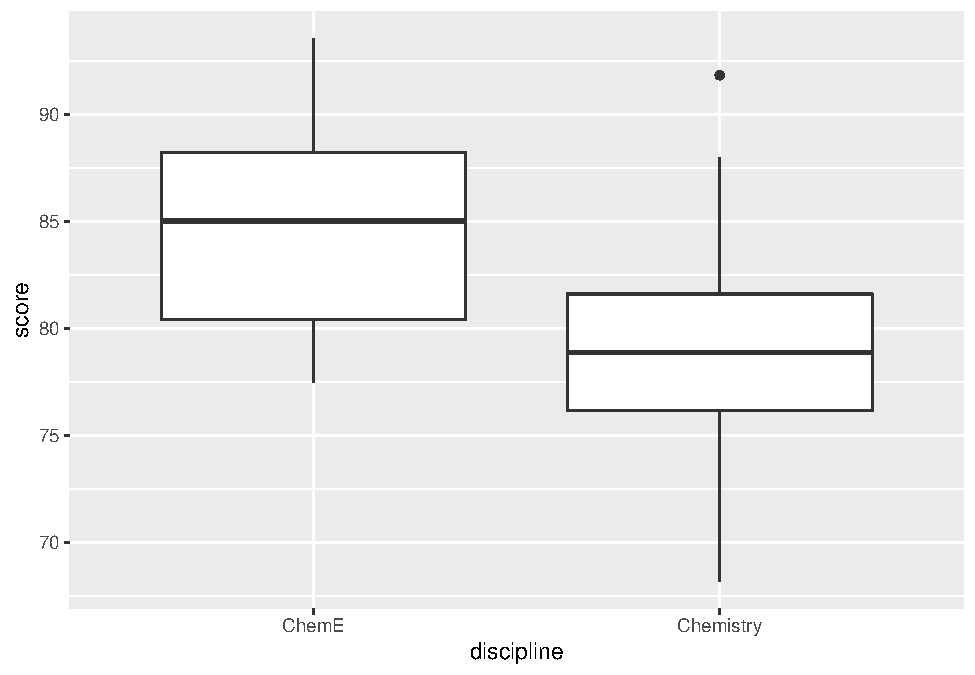
\includegraphics{test_course_notes_files/figure-latex/unnamed-chunk-38-1.pdf}

You can make a few modifications to possibly make this plot easier to read.

The first is to put the discrete category on the y axis instead of the x axis.

The second is to use geom\_jitter() in addition to geom\_boxplot() to show the individual points in each group.

\begin{Shaded}
\begin{Highlighting}[]
\NormalTok{data\_df }\SpecialCharTok{\%\textgreater{}\%} 
  \FunctionTok{ggplot}\NormalTok{(}\FunctionTok{aes}\NormalTok{(}\AttributeTok{y =}\NormalTok{ score, }\AttributeTok{x =}\NormalTok{ discipline)) }\SpecialCharTok{+}
  \FunctionTok{geom\_boxplot}\NormalTok{() }\SpecialCharTok{+}
  \FunctionTok{geom\_jitter}\NormalTok{()}
\end{Highlighting}
\end{Shaded}

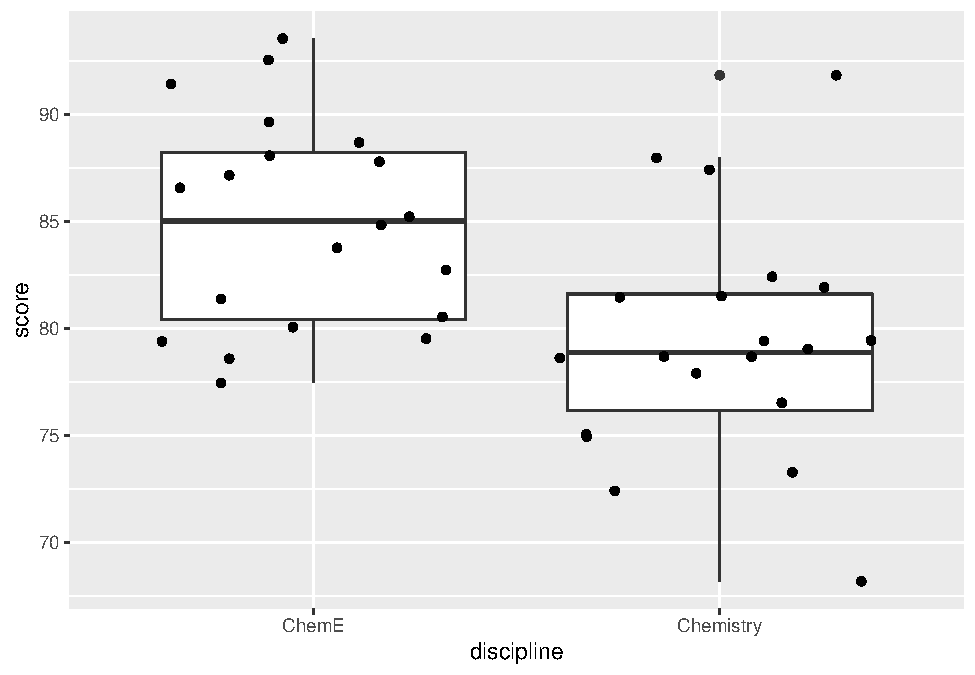
\includegraphics{test_course_notes_files/figure-latex/box-and-dot-plot-1.pdf}

\hypertarget{continuous-predictor-and-continuous-outcome}{%
\section{Continuous predictor and continuous outcome}\label{continuous-predictor-and-continuous-outcome}}

First, let's re-do a lot of the steps in this week's script for reading in data and transforming it a little

\begin{Shaded}
\begin{Highlighting}[]
\NormalTok{mydata }\OtherTok{\textless{}{-}} \FunctionTok{read\_csv}\NormalTok{(}\StringTok{"Free Reduced Lunch by Schools and Grade Structures 2008{-}2017\_final.csv"}\NormalTok{)}
\end{Highlighting}
\end{Shaded}

\begin{verbatim}
## Parsed with column specification:
## cols(
##   .default = col_character(),
##   div_num = col_double()
## )
\end{verbatim}

\begin{verbatim}
## See spec(...) for full column specifications.
\end{verbatim}

Check the structure of the data (this output is a bit long).

\begin{Shaded}
\begin{Highlighting}[]
\FunctionTok{str}\NormalTok{(mydata)}
\end{Highlighting}
\end{Shaded}

\begin{verbatim}
## tibble [2,101 x 137] (S3: spec_tbl_df/tbl_df/tbl/data.frame)
##  $ sch_id        : chr [1:2101] "001-0070" "001-0080" "001-0530" "001-0540" ...
##  $ div_num       : num [1:2101] 1 1 1 1 1 1 1 1 1 1 ...
##  $ div_name      : chr [1:2101] "Accomack County" "Accomack County" "Accomack County" "Accomack County" ...
##  $ school_num    : chr [1:2101] "0070<U+00A0>" "0080<U+00A0>" "0530<U+00A0>" "0540<U+00A0>" ...
##  $ school_name   : chr [1:2101] "NANDUA HIGH" "CHINCOTEAGUE ELEM" "TANGIER COMBINED" "ARCADIA HIGH" ...
##  $ school_name2  : chr [1:2101] NA NA NA NA ...
##  $ type0809      : chr [1:2101] "SCH-HIGH" "SCH-ELEM" "SCH-COMB" "SCH-HIGH" ...
##  $ lowgrade_2008 : chr [1:2101] "9" "PK" "KG" "9" ...
##  $ higrade_2008  : chr [1:2101] "12" "5" "12" "12" ...
##  $ totalFT_2008  : chr [1:2101] "731" "263" "80" "638" ...
##  $ total_2008    : chr [1:2101] "731" "263" "80" "638" ...
##  $ snp_0809      : chr [1:2101] "659" "257" "80" "622" ...
##  $ free_elig_0809: chr [1:2101] "306" "95" "38" "289" ...
##  $ free_per_0809 : chr [1:2101] "46.43%" "36.96%" "47.50%" "46.46%" ...
##  $ red_elig_0809 : chr [1:2101] "64" "8" "0" "56" ...
##  $ red_per_0809  : chr [1:2101] "9.71%" "3.11%" "0.00%" "9.00%" ...
##  $ totalFRL_0809 : chr [1:2101] "370" "103" "38" "345" ...
##  $ totalper_0809 : chr [1:2101] "56.15%" "40.08%" "47.50%" "55.47%" ...
##  $ type0910      : chr [1:2101] "SCH-HIGH" "SCH-ELEM" "SCH-COMB" "SCH-HIGH" ...
##  $ lowgrade_2009 : chr [1:2101] "9" "PK" "KG" "9" ...
##  $ higrade_2009  : chr [1:2101] "12" "5" "12" "12" ...
##  $ totalFT_2009  : chr [1:2101] "654" "266" "78" "634" ...
##  $ total_2009    : chr [1:2101] "654" "266" "78" "634" ...
##  $ snp_0910      : chr [1:2101] "655" "266" "78" "635" ...
##  $ free_elig_0910: chr [1:2101] "290" "99" "36" "286" ...
##  $ free_per_0910 : chr [1:2101] "44.27%" "37.22%" "46.15%" "45.04%" ...
##  $ red_elig_0910 : chr [1:2101] "37" "14" "0" "66" ...
##  $ red_per_0910  : chr [1:2101] "5.65%" "5.26%" "0.00%" "10.39%" ...
##  $ totalFRL_09010: chr [1:2101] "327" "113" "36" "352" ...
##  $ totalper_0910 : chr [1:2101] "49.92%" "42.48%" "46.15%" "55.43%" ...
##  $ type1011      : chr [1:2101] "SCH-HIGH" "SCH-ELEM" "SCH-COMB" "SCH-HIGH" ...
##  $ lowgrade_2010 : chr [1:2101] "9" "PK" "KG" "9" ...
##  $ higrade_2010  : chr [1:2101] "12" "5" "12" "12" ...
##  $ totalFT_2010  : chr [1:2101] "603" "268" "74" "614" ...
##  $ total_2010    : chr [1:2101] "603" "268" "74" "614" ...
##  $ snp_1011      : chr [1:2101] "603" "277" "74" "606" ...
##  $ free_elig_1011: chr [1:2101] "285" "108" "32" "308" ...
##  $ free_per_1011 : chr [1:2101] "47.26%" "38.99%" "43.24%" "50.83%" ...
##  $ red_elig_1011 : chr [1:2101] "46" "8" "0" "50" ...
##  $ red_per_1011  : chr [1:2101] "7.63%" "2.89%" "0.00%" "8.25%" ...
##  $ totalFRL_1011 : chr [1:2101] "331" "116" "32" "358" ...
##  $ totalper_1011 : chr [1:2101] "54.89%" "41.88%" "43.24%" "59.08%" ...
##  $ type1112      : chr [1:2101] "SCH-HIGH" "SCH-ELEM" "SCH-COMB" "SCH-HIGH" ...
##  $ lowgrade_2011 : chr [1:2101] "9" "PK" "KG" "9" ...
##  $ higrade_2011  : chr [1:2101] "12" "5" "12" "12" ...
##  $ totalFT_2011  : chr [1:2101] "593" "276" "73" "605" ...
##  $ total_2011    : chr [1:2101] "593" "276" "73" "605" ...
##  $ snp_1112      : chr [1:2101] "593" "281" "73" "611" ...
##  $ free_elig_1112: chr [1:2101] "289" "116" "31" "318" ...
##  $ free_per_1112 : chr [1:2101] "48.74%" "41.28%" "42.47%" "52.05%" ...
##  $ red_elig_1112 : chr [1:2101] "50" "14" "0" "44" ...
##  $ red_per_1112  : chr [1:2101] "8.43%" "4.98%" "0.00%" "7.20%" ...
##  $ totalFRL_1112 : chr [1:2101] "339" "130" "31" "362" ...
##  $ totalper_1112 : chr [1:2101] "57.17%" "46.26%" "42.47%" "59.25%" ...
##  $ type1213      : chr [1:2101] "SCH-HIGH" "SCH-ELEM" "SCH-COMB" "SCH-HIGH" ...
##  $ lowgrade_2012 : chr [1:2101] "9" "PK" "KG" "9" ...
##  $ higrade_2012  : chr [1:2101] "12" "5" "12" "12" ...
##  $ totalFT_2012  : chr [1:2101] "637" "258" "68" "579" ...
##  $ total_2012    : chr [1:2101] "637" "258" "68" "579" ...
##  $ snp_1213      : chr [1:2101] "633" "259" "68" "579" ...
##  $ free_elig_1213: chr [1:2101] "324" "117" "21" "348" ...
##  $ free_per_1213 : chr [1:2101] "51.18%" "45.17%" "30.88%" "60.10%" ...
##  $ red_elig_1213 : chr [1:2101] "42" "20" "5" "33" ...
##  $ red_per_1213  : chr [1:2101] "6.64%" "7.72%" "7.35%" "5.70%" ...
##  $ totalFRL_1213 : chr [1:2101] "366" "137" "26" "381" ...
##  $ totalper_1213 : chr [1:2101] "57.82%" "52.90%" "38.24%" "65.80%" ...
##  $ type1314      : chr [1:2101] "SCH-HIGH" "SCH-ELEM" "SCH-COMB" "SCH-HIGH" ...
##  $ lowgrade_2013 : chr [1:2101] "9" "PK" "KG" "9" ...
##  $ higrade_2013  : chr [1:2101] "12" "5" "12" "12" ...
##  $ totalFT_2013  : chr [1:2101] "670" "238" "66" "582" ...
##  $ total_2013    : chr [1:2101] "670" "238" "66" "582" ...
##  $ snp_1314      : chr [1:2101] "668" "239" "56" "589" ...
##  $ free_elig_1314: chr [1:2101] "346" "102" "12" "347" ...
##  $ free_per_1314 : chr [1:2101] "51.80%" "42.68%" "21.43%" "58.91%" ...
##  $ red_elig_1314 : chr [1:2101] "44" "19" "4" "54" ...
##  $ red_per_1314  : chr [1:2101] "6.59%" "7.95%" "7.14%" "9.17%" ...
##  $ totalFRL_1314 : chr [1:2101] "390" "121" "16" "401" ...
##  $ totalper_1314 : chr [1:2101] "58.38%" "50.63%" "28.57%" "68.08%" ...
##  $ type1415      : chr [1:2101] NA NA NA NA ...
##  $ lowgrade_2014 : chr [1:2101] "9" "PK" "KG" "9" ...
##  $ higrade_2014  : chr [1:2101] "12" "5" "12" "12" ...
##  $ totalFT_2014  : chr [1:2101] "685" "251" "65" "581" ...
##  $ total_2014    : chr [1:2101] "685" "251" "65" "581" ...
##  $ snp_1415      : chr [1:2101] "672" "239" "61" "586" ...
##  $ free_elig_1415: chr [1:2101] "361" "93" "14" "351" ...
##  $ free_per_1415 : chr [1:2101] "53.72%" "38.91%" "22.95%" "59.90%" ...
##  $ red_elig_1415 : chr [1:2101] "40" "17" "4" "40" ...
##  $ red_per_1415  : chr [1:2101] "5.95%" "7.11%" "6.56%" "6.83%" ...
##  $ totalFRL_1415 : chr [1:2101] "401" "110" "18" "391" ...
##  $ totalper_1415 : chr [1:2101] "59.67%" "46.03%" "29.51%" "66.72%" ...
##  $ CEP_1516      : chr [1:2101] "#NULL!" "#NULL!" "#NULL!" "#NULL!" ...
##  $ type1516      : chr [1:2101] "SCH-HIGH" "SCH-ELEM" "SCH-COMB" "SCH-HIGH" ...
##  $ lowgrade_2015 : chr [1:2101] "9" "PK" "KG" "9" ...
##  $ higrade_2015  : chr [1:2101] "12" "5" "12" "12" ...
##  $ totalFT_2015  : chr [1:2101] "737" "259" "65" "621" ...
##  $ total_2015    : chr [1:2101] "737" "259" "65" "621" ...
##  $ snp_1516      : chr [1:2101] "728" "268" "67" "608" ...
##  $ free_elig_1516: chr [1:2101] "362" "109" "12" "339" ...
##  $ free_per_1516 : chr [1:2101] "49.73%" "40.67%" "17.91%" "55.76%" ...
##   [list output truncated]
##  - attr(*, "spec")=
##   .. cols(
##   ..   sch_id = col_character(),
##   ..   div_num = col_double(),
##   ..   div_name = col_character(),
##   ..   school_num = col_character(),
##   ..   school_name = col_character(),
##   ..   school_name2 = col_character(),
##   ..   type0809 = col_character(),
##   ..   lowgrade_2008 = col_character(),
##   ..   higrade_2008 = col_character(),
##   ..   totalFT_2008 = col_character(),
##   ..   total_2008 = col_character(),
##   ..   snp_0809 = col_character(),
##   ..   free_elig_0809 = col_character(),
##   ..   free_per_0809 = col_character(),
##   ..   red_elig_0809 = col_character(),
##   ..   red_per_0809 = col_character(),
##   ..   totalFRL_0809 = col_character(),
##   ..   totalper_0809 = col_character(),
##   ..   type0910 = col_character(),
##   ..   lowgrade_2009 = col_character(),
##   ..   higrade_2009 = col_character(),
##   ..   totalFT_2009 = col_character(),
##   ..   total_2009 = col_character(),
##   ..   snp_0910 = col_character(),
##   ..   free_elig_0910 = col_character(),
##   ..   free_per_0910 = col_character(),
##   ..   red_elig_0910 = col_character(),
##   ..   red_per_0910 = col_character(),
##   ..   totalFRL_09010 = col_character(),
##   ..   totalper_0910 = col_character(),
##   ..   type1011 = col_character(),
##   ..   lowgrade_2010 = col_character(),
##   ..   higrade_2010 = col_character(),
##   ..   totalFT_2010 = col_character(),
##   ..   total_2010 = col_character(),
##   ..   snp_1011 = col_character(),
##   ..   free_elig_1011 = col_character(),
##   ..   free_per_1011 = col_character(),
##   ..   red_elig_1011 = col_character(),
##   ..   red_per_1011 = col_character(),
##   ..   totalFRL_1011 = col_character(),
##   ..   totalper_1011 = col_character(),
##   ..   type1112 = col_character(),
##   ..   lowgrade_2011 = col_character(),
##   ..   higrade_2011 = col_character(),
##   ..   totalFT_2011 = col_character(),
##   ..   total_2011 = col_character(),
##   ..   snp_1112 = col_character(),
##   ..   free_elig_1112 = col_character(),
##   ..   free_per_1112 = col_character(),
##   ..   red_elig_1112 = col_character(),
##   ..   red_per_1112 = col_character(),
##   ..   totalFRL_1112 = col_character(),
##   ..   totalper_1112 = col_character(),
##   ..   type1213 = col_character(),
##   ..   lowgrade_2012 = col_character(),
##   ..   higrade_2012 = col_character(),
##   ..   totalFT_2012 = col_character(),
##   ..   total_2012 = col_character(),
##   ..   snp_1213 = col_character(),
##   ..   free_elig_1213 = col_character(),
##   ..   free_per_1213 = col_character(),
##   ..   red_elig_1213 = col_character(),
##   ..   red_per_1213 = col_character(),
##   ..   totalFRL_1213 = col_character(),
##   ..   totalper_1213 = col_character(),
##   ..   type1314 = col_character(),
##   ..   lowgrade_2013 = col_character(),
##   ..   higrade_2013 = col_character(),
##   ..   totalFT_2013 = col_character(),
##   ..   total_2013 = col_character(),
##   ..   snp_1314 = col_character(),
##   ..   free_elig_1314 = col_character(),
##   ..   free_per_1314 = col_character(),
##   ..   red_elig_1314 = col_character(),
##   ..   red_per_1314 = col_character(),
##   ..   totalFRL_1314 = col_character(),
##   ..   totalper_1314 = col_character(),
##   ..   type1415 = col_character(),
##   ..   lowgrade_2014 = col_character(),
##   ..   higrade_2014 = col_character(),
##   ..   totalFT_2014 = col_character(),
##   ..   total_2014 = col_character(),
##   ..   snp_1415 = col_character(),
##   ..   free_elig_1415 = col_character(),
##   ..   free_per_1415 = col_character(),
##   ..   red_elig_1415 = col_character(),
##   ..   red_per_1415 = col_character(),
##   ..   totalFRL_1415 = col_character(),
##   ..   totalper_1415 = col_character(),
##   ..   CEP_1516 = col_character(),
##   ..   type1516 = col_character(),
##   ..   lowgrade_2015 = col_character(),
##   ..   higrade_2015 = col_character(),
##   ..   totalFT_2015 = col_character(),
##   ..   total_2015 = col_character(),
##   ..   snp_1516 = col_character(),
##   ..   free_elig_1516 = col_character(),
##   ..   free_per_1516 = col_character(),
##   ..   red_elig_1516 = col_character(),
##   ..   red_Per_1516 = col_character(),
##   ..   totalFRL_1516 = col_character(),
##   ..   totalper_1516 = col_character(),
##   ..   CEP_1617 = col_character(),
##   ..   type1617 = col_character(),
##   ..   lowgrade_2016 = col_character(),
##   ..   higrade_2016 = col_character(),
##   ..   totalFT_2016 = col_character(),
##   ..   total_2016 = col_character(),
##   ..   snp_2016 = col_character(),
##   ..   free_elig_1617 = col_character(),
##   ..   free_per_1617 = col_character(),
##   ..   red_elig_1617 = col_character(),
##   ..   red_per_1617 = col_character(),
##   ..   totalFRL_1617 = col_character(),
##   ..   totalper_1617 = col_character(),
##   ..   CEP_1718 = col_character(),
##   ..   type1718 = col_character(),
##   ..   lowgrade_2017 = col_character(),
##   ..   higrade_2017 = col_character(),
##   ..   totalFT_2017 = col_character(),
##   ..   total_2017 = col_character(),
##   ..   snp_1718 = col_character(),
##   ..   free_elig_1718 = col_character(),
##   ..   free_per_1718 = col_character(),
##   ..   red_elig_1718 = col_character(),
##   ..   red_per_1718 = col_character(),
##   ..   totalFRL_1718 = col_character(),
##   ..   totalper_1718 = col_character(),
##   ..   stable = col_character(),
##   ..   new = col_character(),
##   ..   closed = col_character(),
##   ..   close_yr = col_character(),
##   ..   reuseid = col_character(),
##   ..   gradechg = col_character(),
##   ..   gradechg_yr = col_character(),
##   ..   grchgyr_2 = col_character()
##   .. )
\end{verbatim}

Or just check the structure of one specific variable.

\begin{Shaded}
\begin{Highlighting}[]
\FunctionTok{str}\NormalTok{(mydata}\SpecialCharTok{$}\NormalTok{total\_2017)}
\end{Highlighting}
\end{Shaded}

\begin{verbatim}
##  chr [1:2101] "742" "236" "60" "624" "286" "485" "583" "550" "600" "514" ...
\end{verbatim}

\textbf{NOTE:} When you have a lot of variables, running this str() function is not a great idea - the output is a little too cumbersome

\hypertarget{mutating-variables}{%
\section{Mutating Variables}\label{mutating-variables}}

Note that almost all of the data reads in as a ``character'' data type which are just strings,
This can create issues.

We know that many of the columns are actually storing numbers or ``numeric'' values as R refers to them.
We need to fix this.

Let's tell R that these columns (at least the two we are going to use) are numeric.

We are going to see two interchangeable ways to do this.

First, we use the \$ operator which lets me specify a specific column within my data frame in combination with the as.numeric() function

\begin{Shaded}
\begin{Highlighting}[]
\NormalTok{mydata}\SpecialCharTok{$}\NormalTok{total\_2017}\OtherTok{\textless{}{-}}\FunctionTok{as.numeric}\NormalTok{(mydata}\SpecialCharTok{$}\NormalTok{total\_2017)}
\NormalTok{mydata}\SpecialCharTok{$}\NormalTok{totalFRL\_1718}\OtherTok{\textless{}{-}}\FunctionTok{as.numeric}\NormalTok{(mydata}\SpecialCharTok{$}\NormalTok{totalFRL\_1718)}
\end{Highlighting}
\end{Shaded}

Some columns have a percent symbol, which you will need to remove before coercing to numeric data type

\begin{Shaded}
\begin{Highlighting}[]
\NormalTok{mydata }\OtherTok{\textless{}{-}}\NormalTok{ mydata }\SpecialCharTok{\%\textgreater{}\%}
  \FunctionTok{mutate}\NormalTok{(}\AttributeTok{totalper\_0809 =} \FunctionTok{str\_remove}\NormalTok{(totalper\_0809, }\StringTok{"\%"}\NormalTok{))}
\end{Highlighting}
\end{Shaded}

Then we can change the column from character to numeric

\begin{Shaded}
\begin{Highlighting}[]
\NormalTok{mydata}\SpecialCharTok{$}\NormalTok{totalper\_0809 }\OtherTok{\textless{}{-}} \FunctionTok{as.numeric}\NormalTok{(mydata}\SpecialCharTok{$}\NormalTok{totalper\_0809)}
\end{Highlighting}
\end{Shaded}

\begin{verbatim}
## Warning: NAs introduced by coercion
\end{verbatim}

Check to make sure it converted the column type correctly using \texttt{str()}.

\begin{Shaded}
\begin{Highlighting}[]
\FunctionTok{str}\NormalTok{(mydata}\SpecialCharTok{$}\NormalTok{totalper\_0809)}
\end{Highlighting}
\end{Shaded}

\begin{verbatim}
##  num [1:2101] 56.1 40.1 47.5 55.5 33.4 ...
\end{verbatim}

Second, alternatively, we can do this for a whole set of variables at once. We just need to specify a matching criteria.

\begin{Shaded}
\begin{Highlighting}[]
\NormalTok{newdf }\OtherTok{\textless{}{-}}\NormalTok{ mydata }\SpecialCharTok{\%\textgreater{}\%} 
  \FunctionTok{mutate\_at}\NormalTok{(}\FunctionTok{vars}\NormalTok{(}\FunctionTok{starts\_with}\NormalTok{(}\StringTok{"total"}\NormalTok{)), as.numeric)}
\end{Highlighting}
\end{Shaded}

\begin{verbatim}
## Warning in mask$eval_all_mutate(dots[[i]]): NAs introduced by coercion

## Warning in mask$eval_all_mutate(dots[[i]]): NAs introduced by coercion

## Warning in mask$eval_all_mutate(dots[[i]]): NAs introduced by coercion

## Warning in mask$eval_all_mutate(dots[[i]]): NAs introduced by coercion

## Warning in mask$eval_all_mutate(dots[[i]]): NAs introduced by coercion

## Warning in mask$eval_all_mutate(dots[[i]]): NAs introduced by coercion

## Warning in mask$eval_all_mutate(dots[[i]]): NAs introduced by coercion

## Warning in mask$eval_all_mutate(dots[[i]]): NAs introduced by coercion

## Warning in mask$eval_all_mutate(dots[[i]]): NAs introduced by coercion

## Warning in mask$eval_all_mutate(dots[[i]]): NAs introduced by coercion

## Warning in mask$eval_all_mutate(dots[[i]]): NAs introduced by coercion

## Warning in mask$eval_all_mutate(dots[[i]]): NAs introduced by coercion

## Warning in mask$eval_all_mutate(dots[[i]]): NAs introduced by coercion

## Warning in mask$eval_all_mutate(dots[[i]]): NAs introduced by coercion

## Warning in mask$eval_all_mutate(dots[[i]]): NAs introduced by coercion

## Warning in mask$eval_all_mutate(dots[[i]]): NAs introduced by coercion

## Warning in mask$eval_all_mutate(dots[[i]]): NAs introduced by coercion

## Warning in mask$eval_all_mutate(dots[[i]]): NAs introduced by coercion

## Warning in mask$eval_all_mutate(dots[[i]]): NAs introduced by coercion

## Warning in mask$eval_all_mutate(dots[[i]]): NAs introduced by coercion

## Warning in mask$eval_all_mutate(dots[[i]]): NAs introduced by coercion

## Warning in mask$eval_all_mutate(dots[[i]]): NAs introduced by coercion

## Warning in mask$eval_all_mutate(dots[[i]]): NAs introduced by coercion

## Warning in mask$eval_all_mutate(dots[[i]]): NAs introduced by coercion

## Warning in mask$eval_all_mutate(dots[[i]]): NAs introduced by coercion

## Warning in mask$eval_all_mutate(dots[[i]]): NAs introduced by coercion

## Warning in mask$eval_all_mutate(dots[[i]]): NAs introduced by coercion

## Warning in mask$eval_all_mutate(dots[[i]]): NAs introduced by coercion

## Warning in mask$eval_all_mutate(dots[[i]]): NAs introduced by coercion

## Warning in mask$eval_all_mutate(dots[[i]]): NAs introduced by coercion

## Warning in mask$eval_all_mutate(dots[[i]]): NAs introduced by coercion

## Warning in mask$eval_all_mutate(dots[[i]]): NAs introduced by coercion

## Warning in mask$eval_all_mutate(dots[[i]]): NAs introduced by coercion

## Warning in mask$eval_all_mutate(dots[[i]]): NAs introduced by coercion

## Warning in mask$eval_all_mutate(dots[[i]]): NAs introduced by coercion

## Warning in mask$eval_all_mutate(dots[[i]]): NAs introduced by coercion

## Warning in mask$eval_all_mutate(dots[[i]]): NAs introduced by coercion
\end{verbatim}

\begin{Shaded}
\begin{Highlighting}[]
\NormalTok{newdf }\OtherTok{\textless{}{-}}\NormalTok{ newdf }\SpecialCharTok{\%\textgreater{}\%} 
  \FunctionTok{mutate\_at}\NormalTok{(}\FunctionTok{vars}\NormalTok{(}\FunctionTok{starts\_with}\NormalTok{(}\StringTok{"totalFRL"}\NormalTok{)), as.numeric)}
\end{Highlighting}
\end{Shaded}

Check whether the old and new variables are stored differently (old as a character, new as a numeric variable)

\begin{Shaded}
\begin{Highlighting}[]
\FunctionTok{str}\NormalTok{(mydata}\SpecialCharTok{$}\NormalTok{total\_2008)}
\end{Highlighting}
\end{Shaded}

\begin{verbatim}
##  chr [1:2101] "731" "263" "80" "638" "333" "536" "610" "490" "585" "450" ...
\end{verbatim}

\begin{Shaded}
\begin{Highlighting}[]
\FunctionTok{str}\NormalTok{(newdf}\SpecialCharTok{$}\NormalTok{total\_2008)}
\end{Highlighting}
\end{Shaded}

\begin{verbatim}
##  num [1:2101] 731 263 80 638 333 536 610 490 585 450 ...
\end{verbatim}

\hypertarget{filtering-and-selecting}{%
\section{Filtering and Selecting}\label{filtering-and-selecting}}

A basic operation we do a lot is to filter the data so that we are working with a subset of all that we have.

We can do this with the filter() function, part of the dplyr package (in the tidyverse collection of packages).

Let's say we want to look at the schools with div\_num values less than 50.

\begin{Shaded}
\begin{Highlighting}[]
\NormalTok{newdf }\SpecialCharTok{\%\textgreater{}\%} \FunctionTok{filter}\NormalTok{(div\_num }\SpecialCharTok{\textless{}} \DecValTok{50}\NormalTok{)}
\end{Highlighting}
\end{Shaded}

\begin{verbatim}
## # A tibble: 800 x 137
##    sch_id div_num div_name school_num school_name school_name2 type0809
##    <chr>    <dbl> <chr>    <chr>      <chr>       <chr>        <chr>   
##  1 001-0~       1 Accomac~ "0070\xa0" NANDUA HIGH <NA>         SCH-HIGH
##  2 001-0~       1 Accomac~ "0080\xa0" CHINCOTEAG~ <NA>         SCH-ELEM
##  3 001-0~       1 Accomac~ "0530\xa0" TANGIER CO~ <NA>         SCH-COMB
##  4 001-0~       1 Accomac~ "0540\xa0" ARCADIA HI~ <NA>         SCH-HIGH
##  5 001-0~       1 Accomac~ "0580\xa0" CHINCOTEAG~ <NA>         SCH-COMB
##  6 001-0~       1 Accomac~ "0590\xa0" PUNGOTEAGU~ <NA>         SCH-ELEM
##  7 001-0~       1 Accomac~ "0600\xa0" KEGOTANK E~ <NA>         SCH-ELEM
##  8 001-0~       1 Accomac~ "0701\xa0" ACCAWMACKE~ <NA>         SCH-ELEM
##  9 001-0~       1 Accomac~ "0702\xa0" METOMPKIN ~ <NA>         SCH-ELEM
## 10 001-0~       1 Accomac~ "0703\xa0" NANDUA MID~ <NA>         SCH-MID 
## # ... with 790 more rows, and 130 more variables: lowgrade_2008 <chr>,
## #   higrade_2008 <chr>, totalFT_2008 <dbl>, total_2008 <dbl>, snp_0809 <chr>,
## #   free_elig_0809 <chr>, free_per_0809 <chr>, red_elig_0809 <chr>,
## #   red_per_0809 <chr>, totalFRL_0809 <dbl>, totalper_0809 <dbl>,
## #   type0910 <chr>, lowgrade_2009 <chr>, higrade_2009 <chr>,
## #   totalFT_2009 <dbl>, total_2009 <dbl>, snp_0910 <chr>, free_elig_0910 <chr>,
## #   free_per_0910 <chr>, red_elig_0910 <chr>, red_per_0910 <chr>,
## #   totalFRL_09010 <dbl>, totalper_0910 <dbl>, type1011 <chr>,
## #   lowgrade_2010 <chr>, higrade_2010 <chr>, totalFT_2010 <dbl>,
## #   total_2010 <dbl>, snp_1011 <chr>, free_elig_1011 <chr>,
## #   free_per_1011 <chr>, red_elig_1011 <chr>, red_per_1011 <chr>,
## #   totalFRL_1011 <dbl>, totalper_1011 <dbl>, type1112 <chr>,
## #   lowgrade_2011 <chr>, higrade_2011 <chr>, totalFT_2011 <dbl>,
## #   total_2011 <dbl>, snp_1112 <chr>, free_elig_1112 <chr>,
## #   free_per_1112 <chr>, red_elig_1112 <chr>, red_per_1112 <chr>,
## #   totalFRL_1112 <dbl>, totalper_1112 <dbl>, type1213 <chr>,
## #   lowgrade_2012 <chr>, higrade_2012 <chr>, totalFT_2012 <dbl>,
## #   total_2012 <dbl>, snp_1213 <chr>, free_elig_1213 <chr>,
## #   free_per_1213 <chr>, red_elig_1213 <chr>, red_per_1213 <chr>,
## #   totalFRL_1213 <dbl>, totalper_1213 <dbl>, type1314 <chr>,
## #   lowgrade_2013 <chr>, higrade_2013 <chr>, totalFT_2013 <dbl>,
## #   total_2013 <dbl>, snp_1314 <chr>, free_elig_1314 <chr>,
## #   free_per_1314 <chr>, red_elig_1314 <chr>, red_per_1314 <chr>,
## #   totalFRL_1314 <dbl>, totalper_1314 <dbl>, type1415 <chr>,
## #   lowgrade_2014 <chr>, higrade_2014 <chr>, totalFT_2014 <dbl>,
## #   total_2014 <dbl>, snp_1415 <chr>, free_elig_1415 <chr>,
## #   free_per_1415 <chr>, red_elig_1415 <chr>, red_per_1415 <chr>,
## #   totalFRL_1415 <dbl>, totalper_1415 <dbl>, CEP_1516 <chr>, type1516 <chr>,
## #   lowgrade_2015 <chr>, higrade_2015 <chr>, totalFT_2015 <dbl>,
## #   total_2015 <dbl>, snp_1516 <chr>, free_elig_1516 <chr>,
## #   free_per_1516 <chr>, red_elig_1516 <chr>, red_Per_1516 <chr>,
## #   totalFRL_1516 <dbl>, totalper_1516 <dbl>, CEP_1617 <chr>, type1617 <chr>,
## #   lowgrade_2016 <chr>, higrade_2016 <chr>, ...
\end{verbatim}

Or, if we want to look at schools where the highest grade in 2008 was grade five, we can try:

\begin{Shaded}
\begin{Highlighting}[]
\NormalTok{newdf }\SpecialCharTok{\%\textgreater{}\%} \FunctionTok{filter}\NormalTok{(higrade\_2008 }\SpecialCharTok{==} \StringTok{"5"}\NormalTok{) }\CommentTok{\# this returns a subsetted dataframe with 878 rows}
\end{Highlighting}
\end{Shaded}

\begin{verbatim}
## # A tibble: 878 x 137
##    sch_id div_num div_name school_num school_name school_name2 type0809
##    <chr>    <dbl> <chr>    <chr>      <chr>       <chr>        <chr>   
##  1 001-0~       1 Accomac~ "0080\xa0" CHINCOTEAG~ <NA>         SCH-ELEM
##  2 001-0~       1 Accomac~ "0590\xa0" PUNGOTEAGU~ <NA>         SCH-ELEM
##  3 001-0~       1 Accomac~ "0600\xa0" KEGOTANK E~ <NA>         SCH-ELEM
##  4 001-0~       1 Accomac~ "0701\xa0" ACCAWMACKE~ <NA>         SCH-ELEM
##  5 001-0~       1 Accomac~ "0702\xa0" METOMPKIN ~ <NA>         SCH-ELEM
##  6 002-0~       2 Albemar~ "0010\xa0" HOLLYMEAD ~ <NA>         SCH-ELEM
##  7 002-0~       2 Albemar~ "0030\xa0" SCOTTSVILL~ <NA>         SCH-ELEM
##  8 002-0~       2 Albemar~ "0040\xa0" MARY CARR ~ <NA>         SCH-ELEM
##  9 002-0~       2 Albemar~ "0100\xa0" BROADUS WO~ <NA>         SCH-ELEM
## 10 002-0~       2 Albemar~ "0150\xa0" PAUL H CAL~ <NA>         SCH-ELEM
## # ... with 868 more rows, and 130 more variables: lowgrade_2008 <chr>,
## #   higrade_2008 <chr>, totalFT_2008 <dbl>, total_2008 <dbl>, snp_0809 <chr>,
## #   free_elig_0809 <chr>, free_per_0809 <chr>, red_elig_0809 <chr>,
## #   red_per_0809 <chr>, totalFRL_0809 <dbl>, totalper_0809 <dbl>,
## #   type0910 <chr>, lowgrade_2009 <chr>, higrade_2009 <chr>,
## #   totalFT_2009 <dbl>, total_2009 <dbl>, snp_0910 <chr>, free_elig_0910 <chr>,
## #   free_per_0910 <chr>, red_elig_0910 <chr>, red_per_0910 <chr>,
## #   totalFRL_09010 <dbl>, totalper_0910 <dbl>, type1011 <chr>,
## #   lowgrade_2010 <chr>, higrade_2010 <chr>, totalFT_2010 <dbl>,
## #   total_2010 <dbl>, snp_1011 <chr>, free_elig_1011 <chr>,
## #   free_per_1011 <chr>, red_elig_1011 <chr>, red_per_1011 <chr>,
## #   totalFRL_1011 <dbl>, totalper_1011 <dbl>, type1112 <chr>,
## #   lowgrade_2011 <chr>, higrade_2011 <chr>, totalFT_2011 <dbl>,
## #   total_2011 <dbl>, snp_1112 <chr>, free_elig_1112 <chr>,
## #   free_per_1112 <chr>, red_elig_1112 <chr>, red_per_1112 <chr>,
## #   totalFRL_1112 <dbl>, totalper_1112 <dbl>, type1213 <chr>,
## #   lowgrade_2012 <chr>, higrade_2012 <chr>, totalFT_2012 <dbl>,
## #   total_2012 <dbl>, snp_1213 <chr>, free_elig_1213 <chr>,
## #   free_per_1213 <chr>, red_elig_1213 <chr>, red_per_1213 <chr>,
## #   totalFRL_1213 <dbl>, totalper_1213 <dbl>, type1314 <chr>,
## #   lowgrade_2013 <chr>, higrade_2013 <chr>, totalFT_2013 <dbl>,
## #   total_2013 <dbl>, snp_1314 <chr>, free_elig_1314 <chr>,
## #   free_per_1314 <chr>, red_elig_1314 <chr>, red_per_1314 <chr>,
## #   totalFRL_1314 <dbl>, totalper_1314 <dbl>, type1415 <chr>,
## #   lowgrade_2014 <chr>, higrade_2014 <chr>, totalFT_2014 <dbl>,
## #   total_2014 <dbl>, snp_1415 <chr>, free_elig_1415 <chr>,
## #   free_per_1415 <chr>, red_elig_1415 <chr>, red_per_1415 <chr>,
## #   totalFRL_1415 <dbl>, totalper_1415 <dbl>, CEP_1516 <chr>, type1516 <chr>,
## #   lowgrade_2015 <chr>, higrade_2015 <chr>, totalFT_2015 <dbl>,
## #   total_2015 <dbl>, snp_1516 <chr>, free_elig_1516 <chr>,
## #   free_per_1516 <chr>, red_elig_1516 <chr>, red_Per_1516 <chr>,
## #   totalFRL_1516 <dbl>, totalper_1516 <dbl>, CEP_1617 <chr>, type1617 <chr>,
## #   lowgrade_2016 <chr>, higrade_2016 <chr>, ...
\end{verbatim}

Note that we had to set it equal to the character value ``5'' rather than the numeric value 5. Why?

If we wanted to filter on numeric values instead, we would want to do something like this:

\begin{Shaded}
\begin{Highlighting}[]
\NormalTok{newdf }\SpecialCharTok{\%\textgreater{}\%} 
  \FunctionTok{mutate}\NormalTok{(}\AttributeTok{higrade\_2008 =} \FunctionTok{as.numeric}\NormalTok{(higrade\_2008)) }\SpecialCharTok{\%\textgreater{}\%} 
  \FunctionTok{filter}\NormalTok{(higrade\_2008 }\SpecialCharTok{==} \DecValTok{5}\NormalTok{) }\CommentTok{\# again, this returns a subsetted dataframe with 878 rows}
\end{Highlighting}
\end{Shaded}

\begin{verbatim}
## Warning in mask$eval_all_mutate(dots[[i]]): NAs introduced by coercion
\end{verbatim}

\begin{verbatim}
## # A tibble: 878 x 137
##    sch_id div_num div_name school_num school_name school_name2 type0809
##    <chr>    <dbl> <chr>    <chr>      <chr>       <chr>        <chr>   
##  1 001-0~       1 Accomac~ "0080\xa0" CHINCOTEAG~ <NA>         SCH-ELEM
##  2 001-0~       1 Accomac~ "0590\xa0" PUNGOTEAGU~ <NA>         SCH-ELEM
##  3 001-0~       1 Accomac~ "0600\xa0" KEGOTANK E~ <NA>         SCH-ELEM
##  4 001-0~       1 Accomac~ "0701\xa0" ACCAWMACKE~ <NA>         SCH-ELEM
##  5 001-0~       1 Accomac~ "0702\xa0" METOMPKIN ~ <NA>         SCH-ELEM
##  6 002-0~       2 Albemar~ "0010\xa0" HOLLYMEAD ~ <NA>         SCH-ELEM
##  7 002-0~       2 Albemar~ "0030\xa0" SCOTTSVILL~ <NA>         SCH-ELEM
##  8 002-0~       2 Albemar~ "0040\xa0" MARY CARR ~ <NA>         SCH-ELEM
##  9 002-0~       2 Albemar~ "0100\xa0" BROADUS WO~ <NA>         SCH-ELEM
## 10 002-0~       2 Albemar~ "0150\xa0" PAUL H CAL~ <NA>         SCH-ELEM
## # ... with 868 more rows, and 130 more variables: lowgrade_2008 <chr>,
## #   higrade_2008 <dbl>, totalFT_2008 <dbl>, total_2008 <dbl>, snp_0809 <chr>,
## #   free_elig_0809 <chr>, free_per_0809 <chr>, red_elig_0809 <chr>,
## #   red_per_0809 <chr>, totalFRL_0809 <dbl>, totalper_0809 <dbl>,
## #   type0910 <chr>, lowgrade_2009 <chr>, higrade_2009 <chr>,
## #   totalFT_2009 <dbl>, total_2009 <dbl>, snp_0910 <chr>, free_elig_0910 <chr>,
## #   free_per_0910 <chr>, red_elig_0910 <chr>, red_per_0910 <chr>,
## #   totalFRL_09010 <dbl>, totalper_0910 <dbl>, type1011 <chr>,
## #   lowgrade_2010 <chr>, higrade_2010 <chr>, totalFT_2010 <dbl>,
## #   total_2010 <dbl>, snp_1011 <chr>, free_elig_1011 <chr>,
## #   free_per_1011 <chr>, red_elig_1011 <chr>, red_per_1011 <chr>,
## #   totalFRL_1011 <dbl>, totalper_1011 <dbl>, type1112 <chr>,
## #   lowgrade_2011 <chr>, higrade_2011 <chr>, totalFT_2011 <dbl>,
## #   total_2011 <dbl>, snp_1112 <chr>, free_elig_1112 <chr>,
## #   free_per_1112 <chr>, red_elig_1112 <chr>, red_per_1112 <chr>,
## #   totalFRL_1112 <dbl>, totalper_1112 <dbl>, type1213 <chr>,
## #   lowgrade_2012 <chr>, higrade_2012 <chr>, totalFT_2012 <dbl>,
## #   total_2012 <dbl>, snp_1213 <chr>, free_elig_1213 <chr>,
## #   free_per_1213 <chr>, red_elig_1213 <chr>, red_per_1213 <chr>,
## #   totalFRL_1213 <dbl>, totalper_1213 <dbl>, type1314 <chr>,
## #   lowgrade_2013 <chr>, higrade_2013 <chr>, totalFT_2013 <dbl>,
## #   total_2013 <dbl>, snp_1314 <chr>, free_elig_1314 <chr>,
## #   free_per_1314 <chr>, red_elig_1314 <chr>, red_per_1314 <chr>,
## #   totalFRL_1314 <dbl>, totalper_1314 <dbl>, type1415 <chr>,
## #   lowgrade_2014 <chr>, higrade_2014 <chr>, totalFT_2014 <dbl>,
## #   total_2014 <dbl>, snp_1415 <chr>, free_elig_1415 <chr>,
## #   free_per_1415 <chr>, red_elig_1415 <chr>, red_per_1415 <chr>,
## #   totalFRL_1415 <dbl>, totalper_1415 <dbl>, CEP_1516 <chr>, type1516 <chr>,
## #   lowgrade_2015 <chr>, higrade_2015 <chr>, totalFT_2015 <dbl>,
## #   total_2015 <dbl>, snp_1516 <chr>, free_elig_1516 <chr>,
## #   free_per_1516 <chr>, red_elig_1516 <chr>, red_Per_1516 <chr>,
## #   totalFRL_1516 <dbl>, totalper_1516 <dbl>, CEP_1617 <chr>, type1617 <chr>,
## #   lowgrade_2016 <chr>, higrade_2016 <chr>, ...
\end{verbatim}

\hypertarget{grouping-and-summarizing}{%
\section{Grouping and Summarizing}\label{grouping-and-summarizing}}

Let's shift gears to a different combination of operations\ldots{}

Let's go ahead and try using tidyverse to narrow to what we want.
Imagine we want to see the county level aggregate numbers for FRL in the 2017-2018 school year.

We will start out with our entire data frame and then use pipes (the \%\textgreater\% operator) to work from there.
The final result will be stored in our new data frame that we are creating, called county\_level\_aggregate.

First, select will pick columns
Next, group\_by and summarize work together to get us our aggregate totals.

\begin{Shaded}
\begin{Highlighting}[]
\NormalTok{county\_level\_aggregate }\OtherTok{\textless{}{-}}\NormalTok{ newdf }\SpecialCharTok{\%\textgreater{}\%} 
  \FunctionTok{select}\NormalTok{(div\_name, total\_2017, totalFRL\_1718) }\SpecialCharTok{\%\textgreater{}\%}
  \FunctionTok{group\_by}\NormalTok{(div\_name) }\SpecialCharTok{\%\textgreater{}\%}
  \FunctionTok{summarize}\NormalTok{(}\AttributeTok{totalstudents =} \FunctionTok{sum}\NormalTok{(total\_2017), }
            \AttributeTok{totalFRL =} \FunctionTok{sum}\NormalTok{(totalFRL\_1718))}
\end{Highlighting}
\end{Shaded}

\begin{verbatim}
## `summarise()` ungrouping output (override with `.groups` argument)
\end{verbatim}

Now, we can compute percentages if we like and we can specify a new column by referring to. One that doesn't exist yet but will after we run this code. We will do this two interchangeable ways.

First, the old school way:

\begin{Shaded}
\begin{Highlighting}[]
\NormalTok{county\_level\_aggregate}\SpecialCharTok{$}\NormalTok{percent\_FRL }\OtherTok{\textless{}{-}}\NormalTok{ county\_level\_aggregate}\SpecialCharTok{$}\NormalTok{totalFRL}\SpecialCharTok{/}\NormalTok{county\_level\_aggregate}\SpecialCharTok{$}\NormalTok{totalstudents}\SpecialCharTok{*}\DecValTok{100}
\end{Highlighting}
\end{Shaded}

Second, the tidyverse way:

\begin{Shaded}
\begin{Highlighting}[]
\NormalTok{county\_level\_aggregate }\OtherTok{\textless{}{-}}\NormalTok{ county\_level\_aggregate }\SpecialCharTok{\%\textgreater{}\%} 
  \FunctionTok{mutate}\NormalTok{(}\AttributeTok{percent\_frl =}\NormalTok{ totalFRL }\SpecialCharTok{/}\NormalTok{ totalstudents }\SpecialCharTok{*} \DecValTok{100}\NormalTok{)}
\end{Highlighting}
\end{Shaded}

Just for fun, let's see how this could have been incorporated into our summarize call

\begin{Shaded}
\begin{Highlighting}[]
\NormalTok{county\_level\_percents }\OtherTok{\textless{}{-}}\NormalTok{ newdf }\SpecialCharTok{\%\textgreater{}\%} 
  \FunctionTok{select}\NormalTok{(div\_name, total\_2017, totalFRL\_1718) }\SpecialCharTok{\%\textgreater{}\%}
  \FunctionTok{group\_by}\NormalTok{(div\_name) }\SpecialCharTok{\%\textgreater{}\%}
  \FunctionTok{summarize}\NormalTok{(}\AttributeTok{percentFRL=}\FunctionTok{sum}\NormalTok{(totalFRL\_1718)}\SpecialCharTok{/}\FunctionTok{sum}\NormalTok{(total\_2017) }\SpecialCharTok{*} \DecValTok{100}\NormalTok{)}
\end{Highlighting}
\end{Shaded}

\begin{verbatim}
## `summarise()` ungrouping output (override with `.groups` argument)
\end{verbatim}

Something is going to look weird with this plot

\begin{Shaded}
\begin{Highlighting}[]
\NormalTok{newdf }\SpecialCharTok{\%\textgreater{}\%} 
  \FunctionTok{ggplot}\NormalTok{(}\FunctionTok{aes}\NormalTok{(totalFRL\_0809, totalFT\_2008)) }\SpecialCharTok{+}
  \FunctionTok{geom\_point}\NormalTok{() }\SpecialCharTok{+}
  \FunctionTok{labs}\NormalTok{(}\AttributeTok{title =} \StringTok{"FRL 2008"}\NormalTok{, }\AttributeTok{x =} \StringTok{"totalFRL\_0809"}\NormalTok{)}
\end{Highlighting}
\end{Shaded}

\begin{verbatim}
## Warning: Removed 236 rows containing missing values (geom_point).
\end{verbatim}

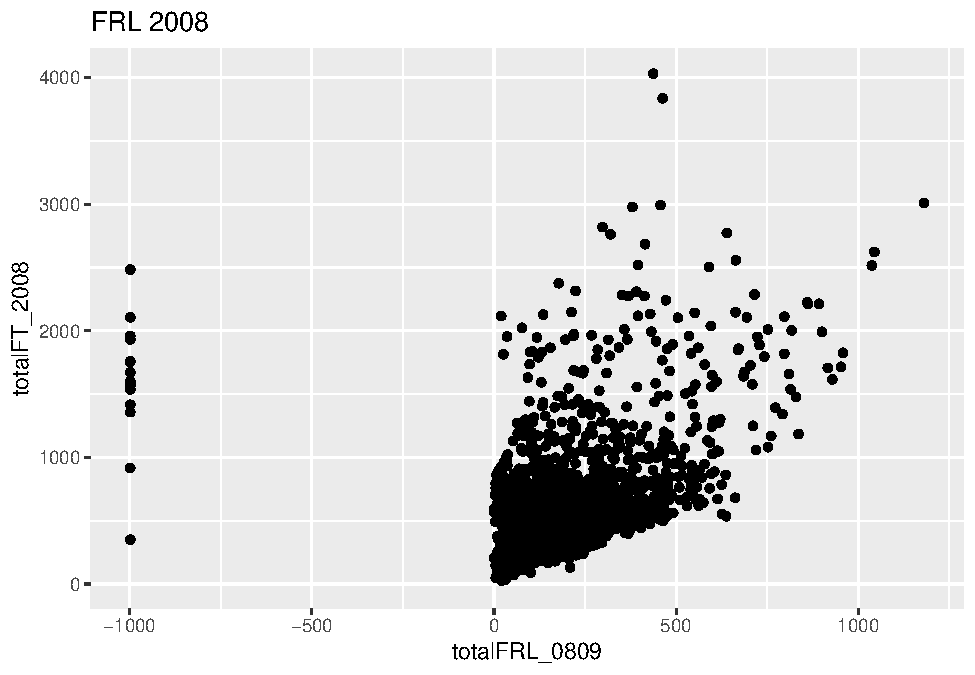
\includegraphics{test_course_notes_files/figure-latex/unnamed-chunk-55-1.pdf}

Let's see if we can fix it

\begin{Shaded}
\begin{Highlighting}[]
\NormalTok{newdf }\SpecialCharTok{\%\textgreater{}\%} 
  \FunctionTok{filter}\NormalTok{(}\SpecialCharTok{!}\FunctionTok{is.na}\NormalTok{(totalFRL\_0809)) }\SpecialCharTok{\%\textgreater{}\%}
  \FunctionTok{ggplot}\NormalTok{(}\FunctionTok{aes}\NormalTok{(totalFRL\_0809, totalFT\_2008)) }\SpecialCharTok{+}
  \FunctionTok{geom\_point}\NormalTok{() }\SpecialCharTok{+}
  \FunctionTok{labs}\NormalTok{(}\AttributeTok{title =} \StringTok{"FRL 2008"}\NormalTok{, }
       \AttributeTok{x =} \StringTok{"totalFRL\_0809"}\NormalTok{) }\SpecialCharTok{+}
  \FunctionTok{xlim}\NormalTok{(}\DecValTok{0}\NormalTok{, }\DecValTok{1000}\NormalTok{) }\SpecialCharTok{+}
  \FunctionTok{ylim}\NormalTok{(}\DecValTok{0}\NormalTok{, }\DecValTok{1000}\NormalTok{)}
\end{Highlighting}
\end{Shaded}

\begin{verbatim}
## Warning: Removed 324 rows containing missing values (geom_point).
\end{verbatim}

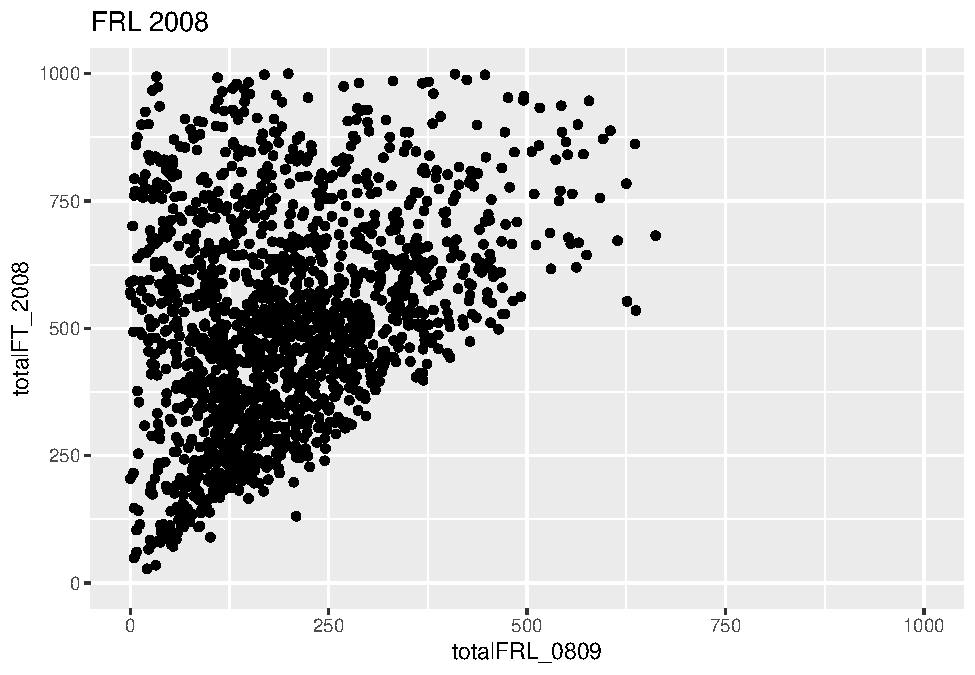
\includegraphics{test_course_notes_files/figure-latex/unnamed-chunk-56-1.pdf}

\hypertarget{week-4-assumptions-and-correlations}{%
\chapter{Week 4: Assumptions and Correlations}\label{week-4-assumptions-and-correlations}}

This week we will be discussing Chapters 5 and 6 from DSUR. These notes will pull out some of the important pieces from each chapter.

\hypertarget{assumptions}{%
\section{Assumptions}\label{assumptions}}

These assumptions that we are making are helpful when determining whether we should be using parametric vs non-parametric statistical tests. What does ``parametric'' mean here? It means that the data are from a parameterized distribution (i.e., parameters characterize the distribution that the data come from). An example of a parameterized distribution that we have already seen is the normal distribution. The two parameters for the normal distribution are \(\mu\) for the mean and \(\sigma\) for the standard deviation. We have seen this altogether with this kind of notation to denote that \(x_i\) is from a normal distribution:

\(x_i \sim \mathcal{N} (\mu, \,\sigma^{2})\)

\hypertarget{normally-distributed-data}{%
\subsection{Normally distributed data}\label{normally-distributed-data}}

This assumption is about the normality of the sampling distribution. The big idea here is that we tend to operate under the belief that if our \emph{sampled} data are normally distributed then the underlying \emph{sampling distribution} is also normally distributed. Also, keep in mind that this becomes less of a concern as our sample size increases (thank, Central Limit Theorem!).

There are several tests for normality that we will discuss, which include either (a) calculations or (b) visual examination. We will discuss both.

\hypertarget{visual-check-of-normality}{%
\subsubsection{Visual check of normality}\label{visual-check-of-normality}}

You can accomplish this with a histogram (e.g., \texttt{hist()} or \texttt{geom\_histogram()} or a q-q plot \texttt{qplot()} (which stands for quantile-quantile).

\hypertarget{homogeneity-of-variance}{%
\subsection{Homogeneity of variance}\label{homogeneity-of-variance}}

Here, you want to know whether the variance of a variable is the same across different groups. For example, if you are looking at test scores in chemistry and chemical engineering students, you want to know if the variances (spread) of the test scores in the chemistry group and the chemical engineering group are close to each other.

\hypertarget{interval-data}{%
\subsection{Interval data}\label{interval-data}}

This might be a little redundant given that we want normally distributed data, but you want at least interval data (ratio data are also fine, but in practice very few things we work with actually qualify as ratio variables). If you have ordinal or nominal variables, you might be in trouble with this assumption\ldots{}

\hypertarget{independence}{%
\subsection{Independence}\label{independence}}

This assumption is about the observations not being related to each other or affecting each other in some way. In practice, this can also be a little tricky. For example, if you are sampling students from different classrooms, depending on the variables you are measuring, you might actually have reason to believe that students in one classroom are more related to each other than students in a different classroom. In practice, you can handle this with a multi-level model (aka hierarchical model), but that is beyond the scope of this class.

\hypertarget{correlation}{%
\section{Correlation}\label{correlation}}

\hypertarget{covariance}{%
\subsection{Covariance}\label{covariance}}

First, start with the observation that variance is calculated with:
\(Variance(s^2) = \frac{\sum(x_i - \overline{x})^2}{N - 1} = \frac{\sum(x_i - \overline{x})(x_i - \overline{x})}{N - 1}\)

But now let's say that we want to know how, for each observation we have, how does the value of \(x\) vary with the value of \(y\) on average. For example, when the value of \(x\) increases, does the value of \(y\) also increase? This could happen when \(x\) represents the number of hours of sleep you get each night and \(y\) is your average grade on an exam you take the next day. The opposite could arise when \(x\) increases but we expect \(y\) to go down. An example of this might be when \(x\) is the number of hilarious jokes that a teacher tells in class and \(y\) is the number of students who fall asleep in class. As the number of jokes increases, we might expect/hope that it keeps students' attention and keeps them from dozing. This generally process of considering how one variable changes when another variable changes is where the notion of covariance comes in.

In practice, what we really want to know is: when \(x_i\) is above its average value in a sample (\(\overline{x}\)), how does \(y_i\) change? Does it also tend to be above the sample average for \(y\) (\(\overline{y}\))? This is expressed in the general formular for covariance:

\(cov(x,y) = \frac{\sum(x_i - \overline{x})(y_i - \overline{y})}{N - 1}\)

While covariance can be a helpful value to work with in many settings, for most of what we do in this class, we will be using correlation coefficients instead of covariance. This is because covariance is an unnormalized value, which can make comparisons across different ranges of values difficult.

\hypertarget{correlation-coefficient}{%
\subsection{Correlation coefficient}\label{correlation-coefficient}}

In order to standardize the covariance to a value the is easier to work with across ranges of values, we use the correlatoin coefficient. There are several version of this, depending on the type of data you are working with. The most basic version is the Pearson correlation coefficient. It is calculated by dividing the covariance by the standard deviations of your two variables of interest:

\(r = \frac{cov_{xy}}{s_xs_y} = \frac{\sum(x_i - \overline{x})(y_i - \overline{y})}{(N-1)s_xs_y}\)

This is a \emph{bivariate} correlation coefficient because it is looking at the correlation between \emph{two variables}. There are also partial correlation coefficients, which look at the correlation between two variables whil controlling for other variables.

We can calculate the correlatoin between two variables using the \texttt{cor()} or \texttt{cor.test()} functions, which are part of base R.

\hypertarget{another-worked-example-for-cleaning-and-prelim-analysis}{%
\section{Another worked example for cleaning and prelim analysis}\label{another-worked-example-for-cleaning-and-prelim-analysis}}

This script takes an incomplete subset of senior data from a .csv file, cleans it,
computes factor scores, and prepares it for analysis.

If you have not already done so, make sure that you have run \texttt{library(tidyverse)} and \texttt{library(psych)} since we will be using functions from both of those packages.

\hypertarget{loading-in-data}{%
\subsection{Loading in data}\label{loading-in-data}}

First, as usual, load in your data. We will use the file \texttt{seniorsurvey.csv} for this demo.

\texttt{file\_path\ \textless{}-\ "YOUR\ PATH\ HERE"}
\texttt{setwd(file\_path)} use this command to change the working directory to the folder where you have your file
\texttt{list.files()} run this to make sure that your file is in your current working directory

\begin{Shaded}
\begin{Highlighting}[]
\NormalTok{seniorSurvey\_df }\OtherTok{\textless{}{-}} \FunctionTok{read\_csv}\NormalTok{(}\StringTok{"seniorsurvey.csv"}\NormalTok{) }\CommentTok{\# replace text in the parentheses with your file name}
\end{Highlighting}
\end{Shaded}

\begin{verbatim}
## Parsed with column specification:
## cols(
##   .default = col_double()
## )
\end{verbatim}

\begin{verbatim}
## See spec(...) for full column specifications.
\end{verbatim}

\hypertarget{data-prep-and-cleaning}{%
\subsection{Data prep and cleaning}\label{data-prep-and-cleaning}}

After loading, it is always nice to just see how things loaded in. Functions like str() and describe() from the psych package are nice for this. For example, if we use describe(), we can see the following (we deleted some variables):

\begin{Shaded}
\begin{Highlighting}[]
\NormalTok{psych}\SpecialCharTok{::}\FunctionTok{describe}\NormalTok{(seniorSurvey\_df)}
\end{Highlighting}
\end{Shaded}

\begin{verbatim}
##                                                   vars    n  mean    sd median
## What is your PRIMARY MAJOR?                          1 1849 31.79 20.43     29
## Internship, field experience, co-op, or practicum    2 1121  1.00  0.00      1
## ParticipateServiceL                                  3  489  1.00  0.00      1
## ParticipateCService                                  4 1296  1.00  0.00      1
## ParticipateStudyAbroadSemester                       5  142  1.00  0.00      1
## SJ1                                                  6 1733  2.32  1.03      2
## SJ2                                                  7 1732  2.08  0.96      2
## SJ3                                                  8 1731  2.77  0.88      3
## SJ4                                                  9 1726  2.27  1.01      2
## SJ5                                                 10 1728  3.27  0.92      3
## SJ6                                                 11 1719  3.50  0.83      4
## SJ7                                                 12 1719  4.01  0.79      4
## SJ8                                                 13 1719  4.15  0.83      4
## DA1                                                 14 1719  2.23  0.93      2
## DA2                                                 15 1719  2.86  0.95      3
## DA3                                                 16 1720  1.97  0.81      2
## DA4                                                 17 1721  4.20  0.72      4
## DA5                                                 18 1721  4.06  0.81      4
## LocalRole                                           19 1453  3.49  0.94      4
## LocalFinance                                        20 1453  3.22  0.90      3
## LocalTime                                           21 1453  3.58  0.89      4
## GlobalRole                                          22 1446  3.57  0.99      4
## GlobalFinance                                       23 1449  3.19  1.00      3
## GlobalTime                                          24 1449  3.42  0.98      3
## Your gender?                                        25 1678  1.49  0.50      1
##                                                   trimmed   mad min max range
## What is your PRIMARY MAJOR?                         31.25 28.17   1  70    69
## Internship, field experience, co-op, or practicum    1.00  0.00   1   1     0
## ParticipateServiceL                                  1.00  0.00   1   1     0
## ParticipateCService                                  1.00  0.00   1   1     0
## ParticipateStudyAbroadSemester                       1.00  0.00   1   1     0
## SJ1                                                  2.25  1.48   1   5     4
## SJ2                                                  1.98  1.48   1   5     4
## SJ3                                                  2.79  1.48   1   5     4
## SJ4                                                  2.20  1.48   1   5     4
## SJ5                                                  3.27  1.48   1   5     4
## SJ6                                                  3.54  1.48   1   5     4
## SJ7                                                  4.07  0.00   1   5     4
## SJ8                                                  4.23  1.48   1   5     4
## DA1                                                  2.15  1.48   1   5     4
## DA2                                                  2.89  1.48   1   5     4
## DA3                                                  1.90  0.00   1   5     4
## DA4                                                  4.27  1.48   1   5     4
## DA5                                                  4.11  1.48   1   5     4
## LocalRole                                            3.51  1.48   1   5     4
## LocalFinance                                         3.23  1.48   1   5     4
## LocalTime                                            3.63  1.48   1   5     4
## GlobalRole                                           3.62  1.48   1   5     4
## GlobalFinance                                        3.18  1.48   1   5     4
## GlobalTime                                           3.44  1.48   1   5     4
## Your gender?                                         1.49  0.00   1   2     1
##                                                    skew kurtosis   se
## What is your PRIMARY MAJOR?                        0.18    -1.33 0.48
## Internship, field experience, co-op, or practicum   NaN      NaN 0.00
## ParticipateServiceL                                 NaN      NaN 0.00
## ParticipateCService                                 NaN      NaN 0.00
## ParticipateStudyAbroadSemester                      NaN      NaN 0.00
## SJ1                                                0.46    -0.51 0.02
## SJ2                                                0.64    -0.16 0.02
## SJ3                                               -0.03    -0.14 0.02
## SJ4                                                0.52    -0.40 0.02
## SJ5                                               -0.19    -0.03 0.02
## SJ6                                               -0.40     0.15 0.02
## SJ7                                               -0.75     1.05 0.02
## SJ8                                               -0.86     0.69 0.02
## DA1                                                0.57    -0.11 0.02
## DA2                                               -0.09    -0.41 0.02
## DA3                                                0.70     0.31 0.02
## DA4                                               -0.66     0.54 0.02
## DA5                                               -0.59     0.16 0.02
## LocalRole                                         -0.44    -0.33 0.02
## LocalFinance                                      -0.19    -0.27 0.02
## LocalTime                                         -0.59     0.22 0.02
## GlobalRole                                        -0.47    -0.30 0.03
## GlobalFinance                                     -0.11    -0.33 0.03
## GlobalTime                                        -0.35    -0.17 0.03
## Your gender?                                       0.03    -2.00 0.01
\end{verbatim}

Upon examining this, we can notice a few things:
Primary Major variable is all messed up. We won't fix it here, but basically there is a numeric code needed (e.g., 13 = underwater basket weaving)

Columns 3 and 5 have lots of missing values (note the small N's) -- this means that this was asked via checkbox so (1) is true and missing is not missing but False

SJ1-8 and DA1-5 all look essentially ok -- about the same N (some survey fatigue or skips) but all values in range (1-5)

Now, we know that SJ and DA are scales from the literature and we want to compute scale scores for those. Typically for attitude scales like these we just report means across the items. So, we will use the ``psych'' package to use a built in function to help us with this. If you have not used psych yet, be sure it is installed using the command install.packages(``psych'') -- you need only do this once and then in subsequent uses you only need \texttt{library(psych)} to tell R to look in that package for the functions you will be using.

\begin{Shaded}
\begin{Highlighting}[]
\FunctionTok{library}\NormalTok{(psych)}
\end{Highlighting}
\end{Shaded}

Subset out only the SJ and DA items in their own dataframe and then use tools in the psych package to compute scale means

The first method to do this - use numbering of the columns:

\begin{Shaded}
\begin{Highlighting}[]
\NormalTok{seniorSurveyScales\_df }\OtherTok{\textless{}{-}}\NormalTok{ seniorSurvey\_df[}\DecValTok{6}\SpecialCharTok{:}\DecValTok{18}\NormalTok{]}
\end{Highlighting}
\end{Shaded}

A second method to do this - use select() from dplyr

\begin{Shaded}
\begin{Highlighting}[]
\NormalTok{seniorSurveyScales\_df }\OtherTok{\textless{}{-}}\NormalTok{ seniorSurvey\_df }\SpecialCharTok{\%\textgreater{}\%} \FunctionTok{select}\NormalTok{(SJ1}\SpecialCharTok{:}\NormalTok{DA5)}
\end{Highlighting}
\end{Shaded}

Use the make.keys() function from psych package to key-in how the scales are built (mapping items to scales, use - for reverse scored items)

\begin{Shaded}
\begin{Highlighting}[]
\NormalTok{my\_keys }\OtherTok{\textless{}{-}} \FunctionTok{make.keys}\NormalTok{(seniorSurveyScales\_df, }\FunctionTok{list}\NormalTok{(}\AttributeTok{SJCa=}\FunctionTok{c}\NormalTok{(}\SpecialCharTok{{-}}\DecValTok{1}\NormalTok{,}\SpecialCharTok{{-}}\DecValTok{2}\NormalTok{,}\SpecialCharTok{{-}}\DecValTok{3}\NormalTok{,}\SpecialCharTok{{-}}\DecValTok{4}\NormalTok{),}\AttributeTok{SJCh=}\FunctionTok{c}\NormalTok{(}\DecValTok{5}\NormalTok{,}\DecValTok{6}\NormalTok{,}\DecValTok{7}\NormalTok{),}\AttributeTok{DA=}\FunctionTok{c}\NormalTok{(}\SpecialCharTok{{-}}\DecValTok{9}\NormalTok{,}\SpecialCharTok{{-}}\DecValTok{10}\NormalTok{,}\SpecialCharTok{{-}}\DecValTok{11}\NormalTok{,}\DecValTok{12}\NormalTok{,}\DecValTok{13}\NormalTok{)))}
\end{Highlighting}
\end{Shaded}

Use scoreItems function to score each respondent on the three scales of interest SJCa, SJCh, and DA -- the default here in scoreItems is to takes the mean of the items (not additive though that is sometimes used) and also, it imputes missing values instead of dropping cases the scoreItems function calculates many things. At this stage, all we really want are the scores, so we include a line to only extract that info.

\begin{Shaded}
\begin{Highlighting}[]
\NormalTok{my\_scales }\OtherTok{\textless{}{-}} \FunctionTok{scoreItems}\NormalTok{(my\_keys, seniorSurveyScales\_df) }
\NormalTok{my\_scores }\OtherTok{\textless{}{-}}\NormalTok{ my\_scales}\SpecialCharTok{$}\NormalTok{scores}
\end{Highlighting}
\end{Shaded}

Now, if you view the first few rows of the my.scores vector using the header -- head() command -- it looks like we expect:

\begin{Shaded}
\begin{Highlighting}[]
\FunctionTok{head}\NormalTok{(my\_scores)}
\end{Highlighting}
\end{Shaded}

\begin{verbatim}
##      SJCa     SJCh  DA
## [1,] 2.75 3.000000 3.2
## [2,] 3.75 3.333333 4.2
## [3,] 3.00 3.000000 3.0
## [4,] 2.25 4.333333 3.6
## [5,] 3.00 3.333333 3.4
## [6,] 4.50 4.333333 3.4
\end{verbatim}

Now, let's build a clean dataframe to prep for analysis - by clean in this case I mean that we have replaced item scores from the scales with their means and also that we have fixed the NAs that don't belong (for participation variables, in this dataset, the NAs should be 0s)

\begin{Shaded}
\begin{Highlighting}[]
\NormalTok{my\_df }\OtherTok{\textless{}{-}} \FunctionTok{data.frame}\NormalTok{(seniorSurvey\_df[}\DecValTok{1}\SpecialCharTok{:}\DecValTok{5}\NormalTok{],my\_scores, seniorSurvey\_df[}\DecValTok{19}\SpecialCharTok{:}\DecValTok{25}\NormalTok{])}
\end{Highlighting}
\end{Shaded}

This is an old school method to replace NAs in specific columns

\begin{Shaded}
\begin{Highlighting}[]
\NormalTok{my\_df}\SpecialCharTok{$}\NormalTok{ParticipateServiceL[}\FunctionTok{is.na}\NormalTok{(my\_df}\SpecialCharTok{$}\NormalTok{ParticipateServiceL)] }\OtherTok{\textless{}{-}} \DecValTok{0} 
\NormalTok{my\_df}\SpecialCharTok{$}\NormalTok{ParticipateCService[}\FunctionTok{is.na}\NormalTok{(my\_df}\SpecialCharTok{$}\NormalTok{ParticipateCService)] }\OtherTok{\textless{}{-}} \DecValTok{0} 
\NormalTok{my\_df}\SpecialCharTok{$}\NormalTok{ParticipateStudyAbroadSemester[}\FunctionTok{is.na}\NormalTok{(my\_df}\SpecialCharTok{$}\NormalTok{ParticipateStudyAbroadSemester)] }\OtherTok{\textless{}{-}} \DecValTok{0} 
\end{Highlighting}
\end{Shaded}

my\_df\(ParticipateInternCoop...[is.na(mydf\)ParticipateInternCoop\ldots){]} \textless- 0 ------- this variable read in cumbersomely named and I don't care about it right now so I'll skip

Here is An alternative method to replace NAs in specific columns:

\begin{Shaded}
\begin{Highlighting}[]
\NormalTok{my\_df }\OtherTok{\textless{}{-}}\NormalTok{ my\_df }\SpecialCharTok{\%\textgreater{}\%} 
  \FunctionTok{replace\_na}\NormalTok{(}\FunctionTok{list}\NormalTok{(}\AttributeTok{ParticipateCService =} \DecValTok{0}\NormalTok{, }\AttributeTok{ParticipateStudyAbroadSemester =} \DecValTok{0}\NormalTok{, }\AttributeTok{ParticipateServiceL =} \DecValTok{0}\NormalTok{))}
\end{Highlighting}
\end{Shaded}

\hypertarget{preliminary-analysis}{%
\subsection{Preliminary analysis}\label{preliminary-analysis}}

At this point, we are ready for some analysis

Let's investigate correlations. What seems most obvious would just be to run cor() but, as we found out in class, this can cause us to run full speed ahead without considering assumptions

\begin{Shaded}
\begin{Highlighting}[]
\NormalTok{my\_correlations }\OtherTok{\textless{}{-}}\NormalTok{ my\_df }\SpecialCharTok{\%\textgreater{}\%} \FunctionTok{select}\NormalTok{(SJCa,SJCh,DA) }\SpecialCharTok{\%\textgreater{}\%} \FunctionTok{cor}\NormalTok{()}
\FunctionTok{print}\NormalTok{(my\_correlations)}
\end{Highlighting}
\end{Shaded}

\begin{verbatim}
##           SJCa      SJCh        DA
## SJCa 1.0000000 0.2590211 0.3342276
## SJCh 0.2590211 1.0000000 0.2310703
## DA   0.3342276 0.2310703 1.0000000
\end{verbatim}

Ok, so, it is important that we note that this ran correlations but R doesn't know that this was sample data and therefore that we are interested instatistical significance (or not) of these results AND that our data may need another method (e.g., non-parametric). cor() does have a way to run spearman instead.

\begin{Shaded}
\begin{Highlighting}[]
\NormalTok{my\_spearman\_correlations }\OtherTok{\textless{}{-}}\NormalTok{ my\_df }\SpecialCharTok{\%\textgreater{}\%} \FunctionTok{select}\NormalTok{(SJCa,SJCh,DA) }\SpecialCharTok{\%\textgreater{}\%} \FunctionTok{cor}\NormalTok{(}\AttributeTok{method=}\StringTok{"spearman"}\NormalTok{)}
\FunctionTok{print}\NormalTok{(my\_spearman\_correlations)}
\end{Highlighting}
\end{Shaded}

\begin{verbatim}
##           SJCa      SJCh        DA
## SJCa 1.0000000 0.2727828 0.3148168
## SJCh 0.2727828 1.0000000 0.2340174
## DA   0.3148168 0.2340174 1.0000000
\end{verbatim}

If we need p values though, we need to change to something else -- corr.test

\begin{Shaded}
\begin{Highlighting}[]
\NormalTok{my\_results }\OtherTok{\textless{}{-}} \FunctionTok{corr.test}\NormalTok{(my\_df}\SpecialCharTok{$}\NormalTok{SJCa,my\_df}\SpecialCharTok{$}\NormalTok{DA)}
\end{Highlighting}
\end{Shaded}

Then we can pull out results from this list or print it. Let's do both.

\begin{Shaded}
\begin{Highlighting}[]
\FunctionTok{print}\NormalTok{(my\_results,}\AttributeTok{short=}\ConstantTok{FALSE}\NormalTok{)}
\end{Highlighting}
\end{Shaded}

\begin{verbatim}
## Call:corr.test(x = my_df$SJCa, y = my_df$DA)
## Correlation matrix 
## [1] 0.33
## Sample Size 
## [1] 1852
## Probability values  adjusted for multiple tests. 
## [1] 0
## 
##  Confidence intervals based upon normal theory.  To get bootstrapped values, try cor.ci
##       raw.lower raw.r raw.upper raw.p lower.adj upper.adj
## NA-NA      0.29  0.33      0.37     0      0.29      0.37
\end{verbatim}

\begin{Shaded}
\begin{Highlighting}[]
\NormalTok{my\_results}\SpecialCharTok{$}\NormalTok{r }\CommentTok{\# correlation coefficient}
\end{Highlighting}
\end{Shaded}

\begin{verbatim}
## [1] 0.3342276
\end{verbatim}

\begin{Shaded}
\begin{Highlighting}[]
\NormalTok{my\_results}\SpecialCharTok{$}\NormalTok{p }\CommentTok{\# p{-}value}
\end{Highlighting}
\end{Shaded}

\begin{verbatim}
## [1] 1.433637e-49
\end{verbatim}

Visually, we should be able to see this on a scatterplot. We are going to use qplot which stands for quickplot from within ggplot. It is useful and quicker for simple plotting than building up ggplot (though from the same package) we need to jitter my points (take geom=``jitter'' out if you want to see why)

\begin{Shaded}
\begin{Highlighting}[]
\FunctionTok{qplot}\NormalTok{(SJCa,DA,}\AttributeTok{data=}\NormalTok{my\_df,}\AttributeTok{geom=}\StringTok{"jitter"}\NormalTok{)}
\end{Highlighting}
\end{Shaded}

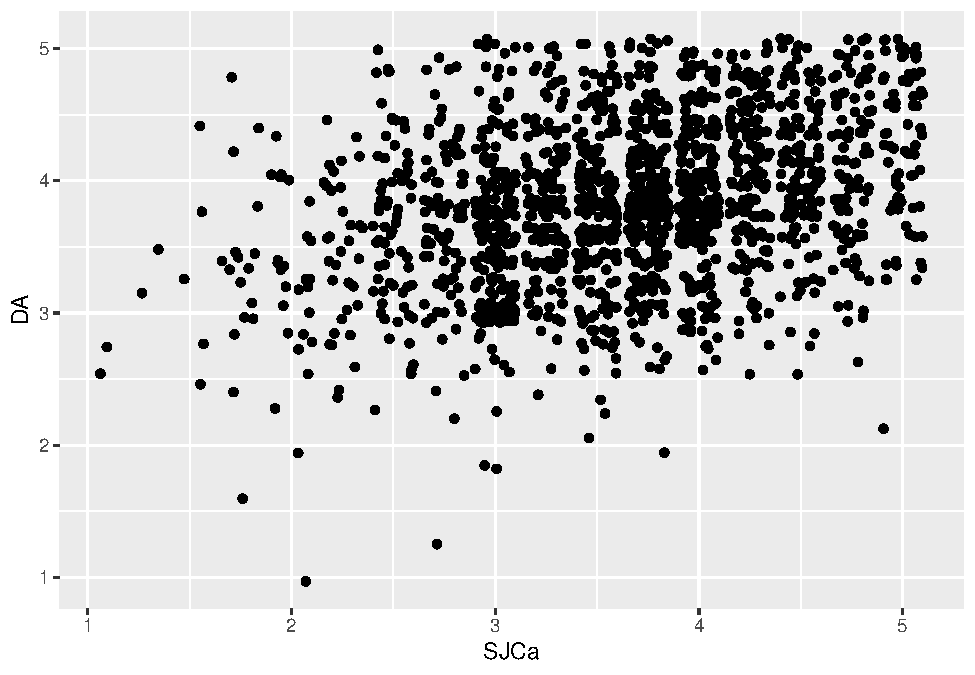
\includegraphics{test_course_notes_files/figure-latex/unnamed-chunk-72-1.pdf}

\begin{Shaded}
\begin{Highlighting}[]
\FunctionTok{qqnorm}\NormalTok{(my\_df}\SpecialCharTok{$}\NormalTok{SJCa, }\AttributeTok{frame =} \ConstantTok{FALSE}\NormalTok{)}
\FunctionTok{qqline}\NormalTok{(my\_df}\SpecialCharTok{$}\NormalTok{SJCa, }\AttributeTok{col =} \StringTok{"steelblue"}\NormalTok{, }\AttributeTok{lwd =} \FloatTok{1.5}\NormalTok{)}
\end{Highlighting}
\end{Shaded}

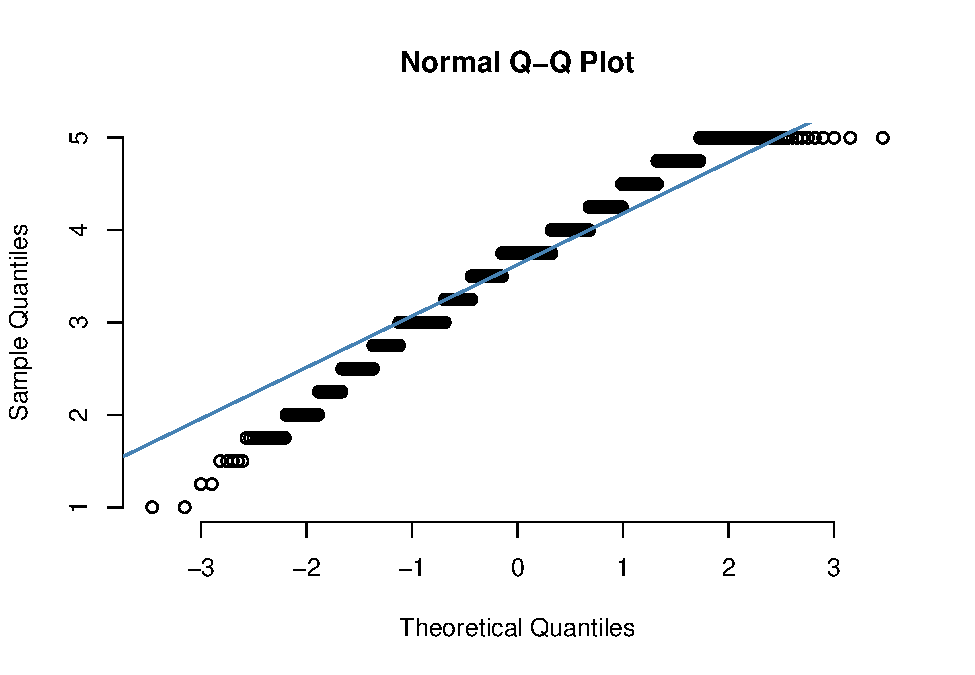
\includegraphics{test_course_notes_files/figure-latex/unnamed-chunk-72-2.pdf}

\begin{Shaded}
\begin{Highlighting}[]
\NormalTok{my\_df }\SpecialCharTok{\%\textgreater{}\%} \FunctionTok{ggplot}\NormalTok{(}\FunctionTok{aes}\NormalTok{(}\AttributeTok{x =}\NormalTok{ SJCa)) }\SpecialCharTok{+}
  \FunctionTok{geom\_histogram}\NormalTok{()}
\end{Highlighting}
\end{Shaded}

\begin{verbatim}
## `stat_bin()` using `bins = 30`. Pick better value with `binwidth`.
\end{verbatim}

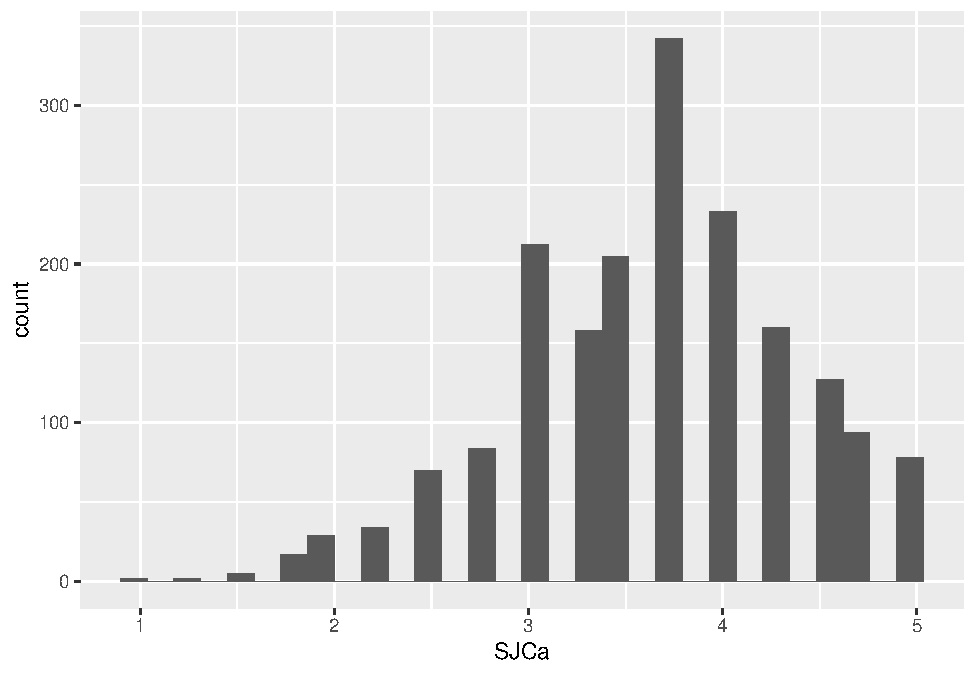
\includegraphics{test_course_notes_files/figure-latex/unnamed-chunk-72-3.pdf}

Other functions we used today in class were describe() and also the q-q plot creation to investigate normality assumption copying syntax from the Field, Miles, \& Field book

\hypertarget{week-5-regression-i}{%
\chapter{Week 5: Regression I}\label{week-5-regression-i}}

Week 5 notes coming soon to an online book near you\ldots{}

\begin{Shaded}
\begin{Highlighting}[]
\FunctionTok{require}\NormalTok{(tidyverse)}
\FunctionTok{require}\NormalTok{(psych)}
\FunctionTok{require}\NormalTok{(kableExtra)}
\end{Highlighting}
\end{Shaded}

\begin{verbatim}
## Loading required package: kableExtra
\end{verbatim}

\begin{verbatim}
## 
## Attaching package: 'kableExtra'
\end{verbatim}

\begin{verbatim}
## The following object is masked from 'package:dplyr':
## 
##     group_rows
\end{verbatim}

\begin{Shaded}
\begin{Highlighting}[]
\FunctionTok{library}\NormalTok{(broom)}
\end{Highlighting}
\end{Shaded}

\hypertarget{week-5---simple-regression}{%
\chapter{Week 5 - Simple Regression}\label{week-5---simple-regression}}

This week we will start learning about linear regression. In particular, we focus on simple regression. These kinds of models involve one predictor variable and one continuous outcome variable. Next week we will move to models with multiple regression, which involves - you guessed it - multiple predictor variables.

\hypertarget{general-modeling-philosophy}{%
\section{General Modeling Philosophy}\label{general-modeling-philosophy}}

The general approach is to model the outcome variable as a function of some predictor(s) plus an error term. Mathematically, this looks like:

\(outcome_i = model + error_i\)

where the \(i\) subscript refers to the \(i^{th}\) person in the sample.

\hypertarget{review-of-the-normal-distribution-and-standardizing-variables}{%
\subsubsection{Review of the normal distribution and standardizing variables}\label{review-of-the-normal-distribution-and-standardizing-variables}}

Just to review, let's think about normally distributed variables and the notion of centering and standardizing.

First, we will generate some data by drawing \texttt{n} random numbers from a normal distribution with a mean and standard deviation that we will specify.

\begin{Shaded}
\begin{Highlighting}[]
\NormalTok{mean }\OtherTok{\textless{}{-}} \DecValTok{5}
\NormalTok{sd }\OtherTok{\textless{}{-}} \DecValTok{3}
\NormalTok{n }\OtherTok{\textless{}{-}} \DecValTok{1000}

\NormalTok{random\_x }\OtherTok{\textless{}{-}} \FunctionTok{rnorm}\NormalTok{(}\AttributeTok{n =}\NormalTok{ n, }\AttributeTok{mean =}\NormalTok{ mean, }\AttributeTok{sd =}\NormalTok{ sd)}
\end{Highlighting}
\end{Shaded}

We can then visualize those numbers

\begin{Shaded}
\begin{Highlighting}[]
\FunctionTok{hist}\NormalTok{(random\_x)}
\end{Highlighting}
\end{Shaded}

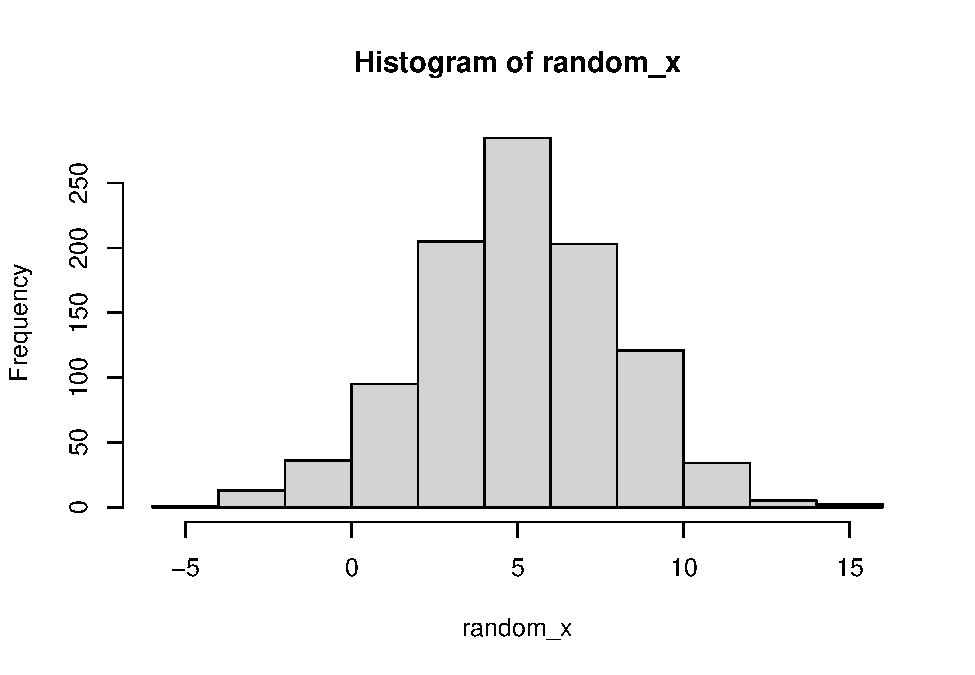
\includegraphics{test_course_notes_files/figure-latex/unnamed-chunk-74-1.pdf}

Now if we subtract the mean and plot the histogram, notice how the values have all basically shifted to the left along the x-axis.

\begin{Shaded}
\begin{Highlighting}[]
\NormalTok{sample\_mean }\OtherTok{\textless{}{-}} \FunctionTok{mean}\NormalTok{(random\_x)}

\NormalTok{centered\_x }\OtherTok{\textless{}{-}}\NormalTok{ random\_x }\SpecialCharTok{{-}}\NormalTok{ sample\_mean}

\FunctionTok{hist}\NormalTok{(centered\_x)}
\end{Highlighting}
\end{Shaded}

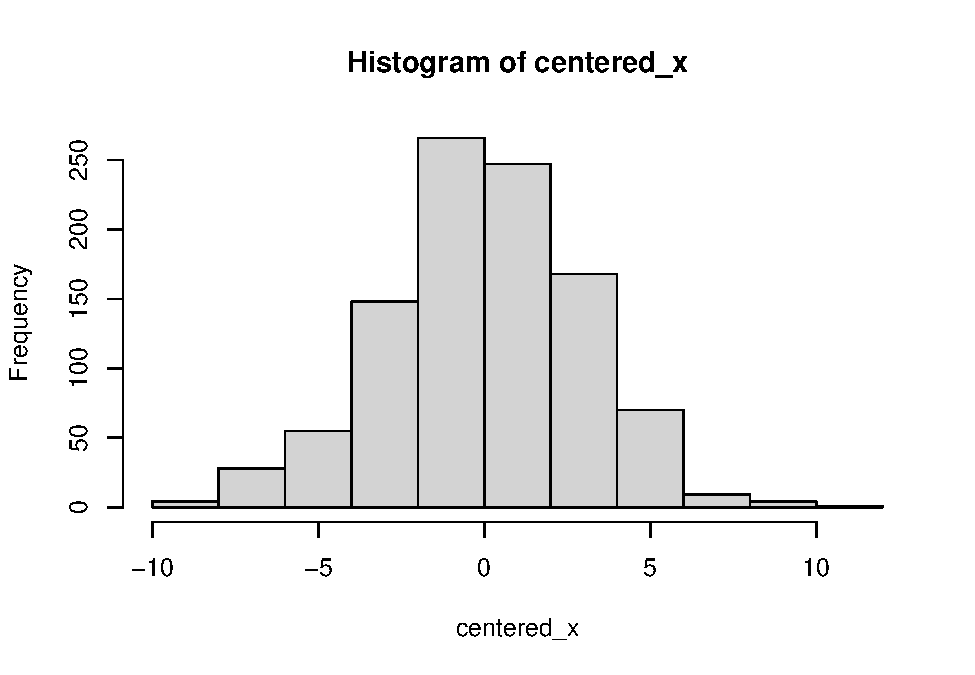
\includegraphics{test_course_notes_files/figure-latex/unnamed-chunk-75-1.pdf}

Finally, we can divide by the sample standard deviation, which should have the effect of either stretching or squishing the values along the x-axis (without changing their mean). Pay attention again to the values along the x-axis.

\begin{Shaded}
\begin{Highlighting}[]
\NormalTok{sample\_sd }\OtherTok{\textless{}{-}} \FunctionTok{sd}\NormalTok{(random\_x)}

\NormalTok{standardized\_x }\OtherTok{\textless{}{-}}\NormalTok{ centered\_x }\SpecialCharTok{/}\NormalTok{ sample\_sd}

\FunctionTok{hist}\NormalTok{(standardized\_x)}
\end{Highlighting}
\end{Shaded}

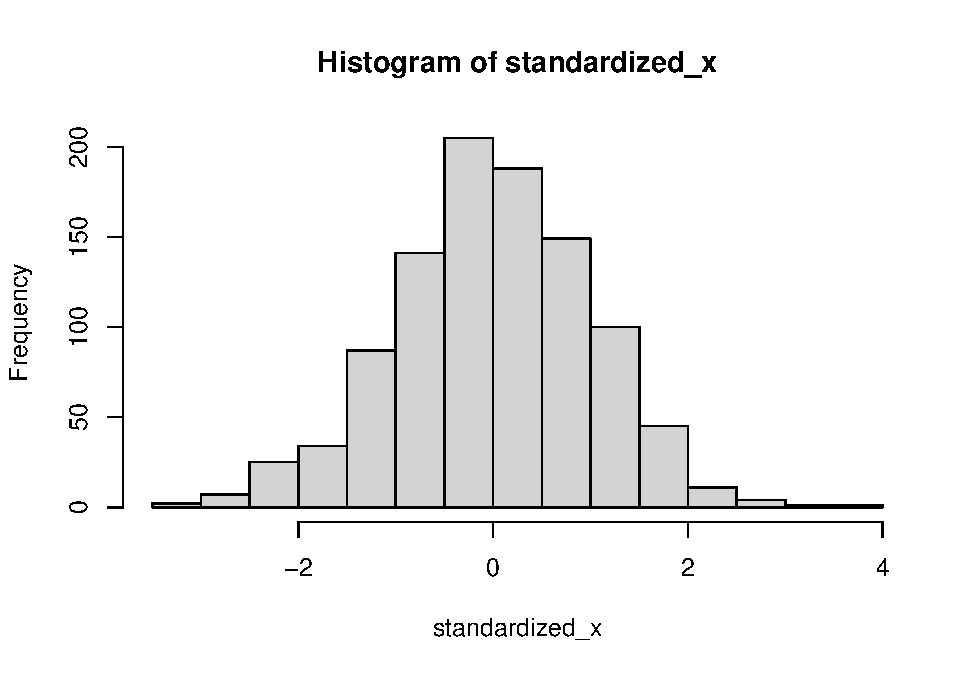
\includegraphics{test_course_notes_files/figure-latex/unnamed-chunk-76-1.pdf}

This final plot should remind you have the standard normal plot (with mean 0 and standard deviation 1). This is noted as \(x \sim \mathcal{N}(0, 1)\) and is read as ``x is distributed according to a normal distribution with a mean of 0 and variance of 1''.

\hypertarget{data-generation-demo---one-set-sample-size}{%
\section{data generation demo - one set sample size}\label{data-generation-demo---one-set-sample-size}}

The following is a demo from class, found in the week\_5\_demo.R file

\begin{Shaded}
\begin{Highlighting}[]
\CommentTok{\#store the sample size that we want to use}
\NormalTok{samp\_size }\OtherTok{\textless{}{-}} \DecValTok{100}
\end{Highlighting}
\end{Shaded}

\begin{Shaded}
\begin{Highlighting}[]
\CommentTok{\# uniformly sample X values (values for our predictor variable) from 0 to 20 }
\NormalTok{x }\OtherTok{\textless{}{-}} \FunctionTok{round}\NormalTok{(}\FunctionTok{runif}\NormalTok{(}\AttributeTok{n =}\NormalTok{ samp\_size, }\AttributeTok{min =} \DecValTok{0}\NormalTok{, }\AttributeTok{max =} \DecValTok{30}\NormalTok{), }\AttributeTok{digits =} \DecValTok{1}\NormalTok{) }\CommentTok{\# this gives samp\_size number of random numbers}
\end{Highlighting}
\end{Shaded}

Store the noise values for our different test models

\begin{Shaded}
\begin{Highlighting}[]
\NormalTok{sd\_min }\OtherTok{\textless{}{-}} \DecValTok{2} \CommentTok{\# low noise}
\NormalTok{sd\_med }\OtherTok{\textless{}{-}} \DecValTok{6} \CommentTok{\# medium noise}
\NormalTok{sd\_max }\OtherTok{\textless{}{-}} \DecValTok{12} \CommentTok{\# high noise}
\end{Highlighting}
\end{Shaded}

Generate the outcome variable values under different amounts of noise (the rnorm() function is what is generating noise here)

\begin{Shaded}
\begin{Highlighting}[]
\NormalTok{y\_noise\_sd\_none }\OtherTok{\textless{}{-}} \DecValTok{3} \SpecialCharTok{+} \DecValTok{2}\SpecialCharTok{*}\NormalTok{x }\CommentTok{\# this is the true relationship without any noise}
\NormalTok{y\_noise\_sd\_min }\OtherTok{\textless{}{-}} \DecValTok{3} \SpecialCharTok{+} \DecValTok{2}\SpecialCharTok{*}\NormalTok{x }\SpecialCharTok{+} \FunctionTok{round}\NormalTok{(}\AttributeTok{x =} \FunctionTok{rnorm}\NormalTok{(}\AttributeTok{n =}\NormalTok{ samp\_size, }\AttributeTok{mean =} \DecValTok{0}\NormalTok{, }\AttributeTok{sd =}\NormalTok{ sd\_min), }\AttributeTok{digits =} \DecValTok{1}\NormalTok{)}
\NormalTok{y\_noise\_sd\_med }\OtherTok{\textless{}{-}} \DecValTok{3} \SpecialCharTok{+} \DecValTok{2}\SpecialCharTok{*}\NormalTok{x }\SpecialCharTok{+} \FunctionTok{round}\NormalTok{(}\AttributeTok{x =} \FunctionTok{rnorm}\NormalTok{(}\AttributeTok{n =}\NormalTok{ samp\_size, }\AttributeTok{mean =} \DecValTok{0}\NormalTok{, }\AttributeTok{sd =}\NormalTok{ sd\_med), }\AttributeTok{digits =} \DecValTok{1}\NormalTok{)}
\NormalTok{y\_noise\_sd\_max }\OtherTok{\textless{}{-}} \DecValTok{3} \SpecialCharTok{+} \DecValTok{2}\SpecialCharTok{*}\NormalTok{x }\SpecialCharTok{+} \FunctionTok{round}\NormalTok{(}\AttributeTok{x =} \FunctionTok{rnorm}\NormalTok{(}\AttributeTok{n =}\NormalTok{ samp\_size, }\AttributeTok{mean =} \DecValTok{0}\NormalTok{, }\AttributeTok{sd =}\NormalTok{ sd\_max), }\AttributeTok{digits =} \DecValTok{1}\NormalTok{)}
\end{Highlighting}
\end{Shaded}

Typical step 1: visualize! Let's plot each of these x values vs y

\begin{Shaded}
\begin{Highlighting}[]
\FunctionTok{plot}\NormalTok{(x, y\_noise\_sd\_none)}
\end{Highlighting}
\end{Shaded}

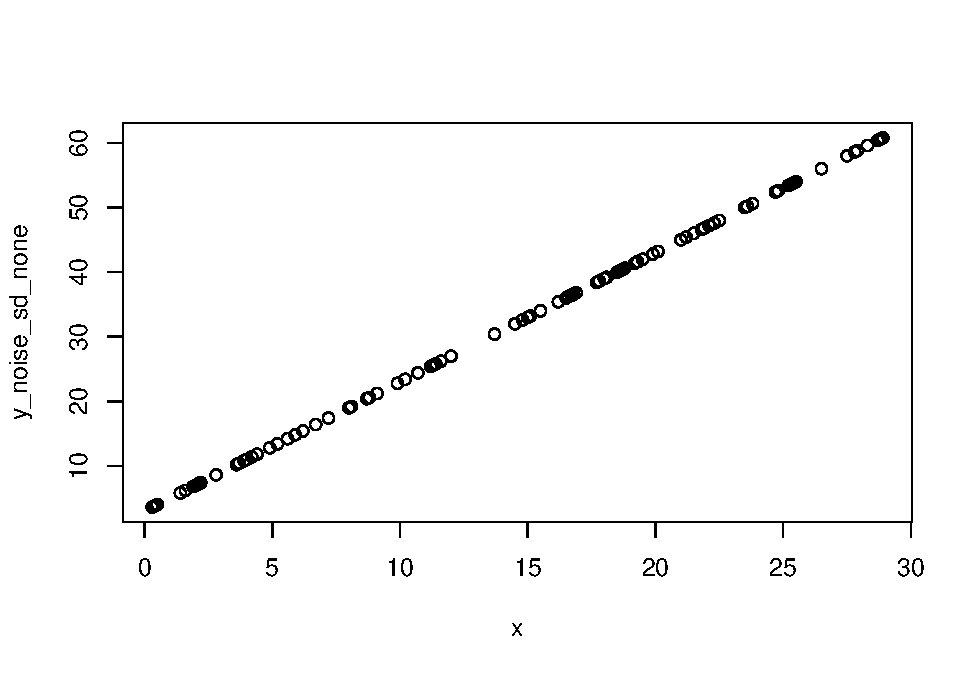
\includegraphics{test_course_notes_files/figure-latex/remedy006-1.pdf}

\begin{Shaded}
\begin{Highlighting}[]
\FunctionTok{plot}\NormalTok{(x, y\_noise\_sd\_min)}
\end{Highlighting}
\end{Shaded}

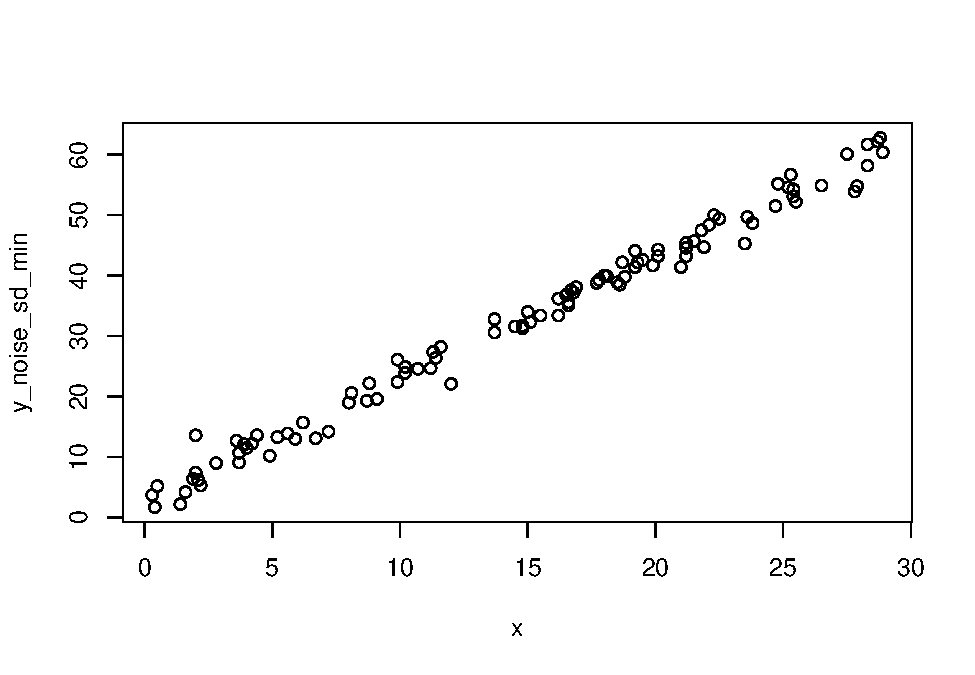
\includegraphics{test_course_notes_files/figure-latex/remedy006-2.pdf}

\begin{Shaded}
\begin{Highlighting}[]
\FunctionTok{plot}\NormalTok{(x, y\_noise\_sd\_med)}
\end{Highlighting}
\end{Shaded}

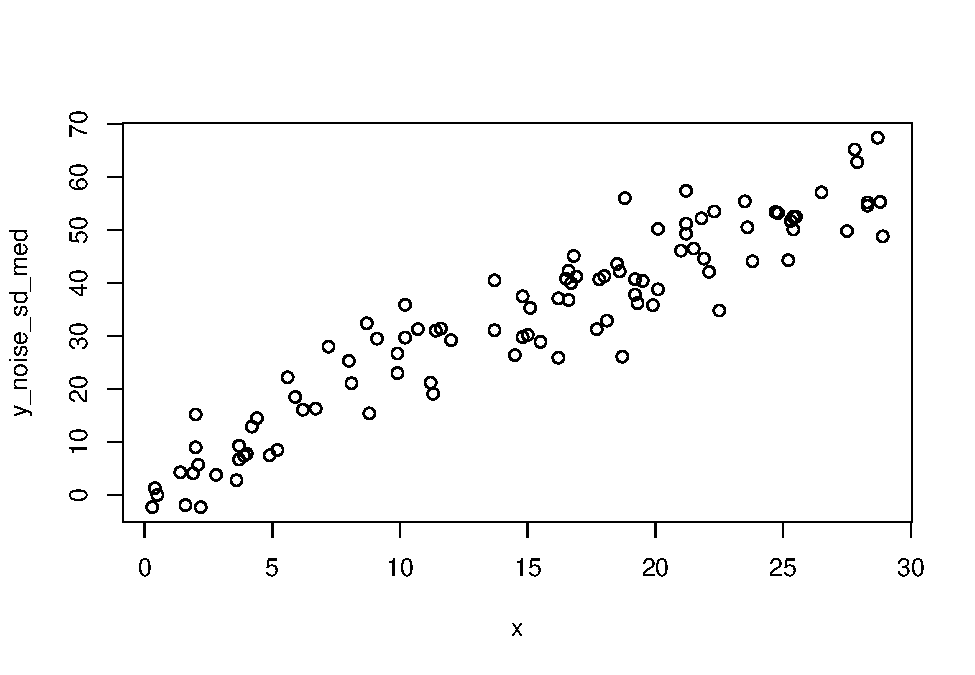
\includegraphics{test_course_notes_files/figure-latex/remedy006-3.pdf}

\begin{Shaded}
\begin{Highlighting}[]
\FunctionTok{plot}\NormalTok{(x, y\_noise\_sd\_max)}
\end{Highlighting}
\end{Shaded}

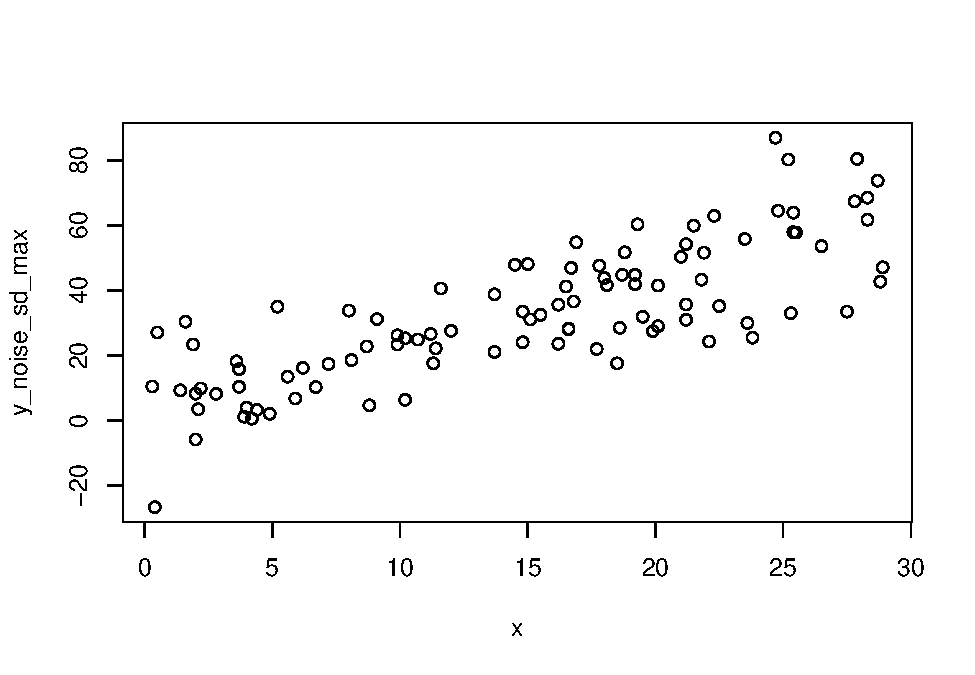
\includegraphics{test_course_notes_files/figure-latex/remedy006-4.pdf}

Let's put all of these vectors together into a data frame to make it easier to analyze later on
Note, this is not a vital step for conducting the simple regression

\begin{Shaded}
\begin{Highlighting}[]
\NormalTok{demo\_df }\OtherTok{\textless{}{-}} \FunctionTok{tibble}\NormalTok{(}\StringTok{"x"} \OtherTok{=}\NormalTok{ x, }
                  \StringTok{"y\_noise\_sd\_none"}\OtherTok{=}\NormalTok{y\_noise\_sd\_none, }
                  \StringTok{"y\_noise\_sd\_min"} \OtherTok{=}\NormalTok{ y\_noise\_sd\_min,}
                  \StringTok{"y\_noise\_sd\_med"} \OtherTok{=}\NormalTok{ y\_noise\_sd\_med,}
                  \StringTok{"y\_noise\_sd\_max"} \OtherTok{=}\NormalTok{ y\_noise\_sd\_max)}
\end{Highlighting}
\end{Shaded}

Check out what demo\_df looks like

\begin{Shaded}
\begin{Highlighting}[]
\FunctionTok{head}\NormalTok{(demo\_df)}
\end{Highlighting}
\end{Shaded}

\begin{verbatim}
## # A tibble: 6 x 5
##       x y_noise_sd_none y_noise_sd_min y_noise_sd_med y_noise_sd_max
##   <dbl>           <dbl>          <dbl>          <dbl>          <dbl>
## 1   9.9            22.8           22.4           26.7           23.4
## 2  28.7            60.4           62.2           67.4           73.7
## 3  22.1            47.2           48.4           42.1           24.3
## 4  21.9            46.8           44.7           44.6           51.6
## 5  17.7            38.4           38.8           31.3           22  
## 6  21              45             41.4           46.1           50.3
\end{verbatim}

Order by increasing x value

\begin{Shaded}
\begin{Highlighting}[]
\NormalTok{demo\_df }\OtherTok{\textless{}{-}}\NormalTok{ demo\_df }\SpecialCharTok{\%\textgreater{}\%} 
  \FunctionTok{arrange}\NormalTok{(x)}
\end{Highlighting}
\end{Shaded}

Check out what the arrange() function did

\begin{Shaded}
\begin{Highlighting}[]
\FunctionTok{head}\NormalTok{(demo\_df)}
\end{Highlighting}
\end{Shaded}

\begin{verbatim}
## # A tibble: 6 x 5
##       x y_noise_sd_none y_noise_sd_min y_noise_sd_med y_noise_sd_max
##   <dbl>           <dbl>          <dbl>          <dbl>          <dbl>
## 1   0.3             3.6           3.7           -2.3            10.5
## 2   0.4             3.8           1.70           1.30          -26.6
## 3   0.5             4             5.2            0              27.1
## 4   1.4             5.8           2.20           4.3             9.3
## 5   1.6             6.2           4.2           -1.90           30.4
## 6   1.9             6.8           6.40           4.1            23.4
\end{verbatim}

Let's make this a long df so that we can plot multiple standard deviation values together

\begin{Shaded}
\begin{Highlighting}[]
\NormalTok{demo\_df\_long }\OtherTok{\textless{}{-}}\NormalTok{ demo\_df }\SpecialCharTok{\%\textgreater{}\%} 
  \FunctionTok{pivot\_longer}\NormalTok{(}\AttributeTok{cols =} \FunctionTok{starts\_with}\NormalTok{(}\StringTok{"y\_noise"}\NormalTok{),}
               \AttributeTok{names\_to =} \StringTok{"y\_col"}\NormalTok{,}
               \AttributeTok{values\_to =} \StringTok{"y\_val"}
\NormalTok{  )}
\end{Highlighting}
\end{Shaded}

Again, check on what this did

\begin{Shaded}
\begin{Highlighting}[]
\FunctionTok{head}\NormalTok{(demo\_df\_long)}
\end{Highlighting}
\end{Shaded}

\begin{verbatim}
## # A tibble: 6 x 3
##       x y_col           y_val
##   <dbl> <chr>           <dbl>
## 1   0.3 y_noise_sd_none  3.6 
## 2   0.3 y_noise_sd_min   3.7 
## 3   0.3 y_noise_sd_med  -2.3 
## 4   0.3 y_noise_sd_max  10.5 
## 5   0.4 y_noise_sd_none  3.8 
## 6   0.4 y_noise_sd_min   1.70
\end{verbatim}

Let's add in a column to note whether the value is from the min, med, max, or zero sd (noise) model

\begin{Shaded}
\begin{Highlighting}[]
\NormalTok{demo\_df\_long }\OtherTok{\textless{}{-}}\NormalTok{ demo\_df\_long }\SpecialCharTok{\%\textgreater{}\%} 
  \FunctionTok{mutate}\NormalTok{(}\AttributeTok{sd\_val =} \FunctionTok{case\_when}\NormalTok{(}\FunctionTok{str\_detect}\NormalTok{(y\_col, }\StringTok{"sd\_none"}\NormalTok{) }\SpecialCharTok{\textasciitilde{}} \DecValTok{0}\NormalTok{,}
                            \FunctionTok{str\_detect}\NormalTok{(y\_col, }\StringTok{"sd\_min"}\NormalTok{) }\SpecialCharTok{\textasciitilde{}}\NormalTok{ sd\_min,}
                            \FunctionTok{str\_detect}\NormalTok{(y\_col, }\StringTok{"sd\_med"}\NormalTok{) }\SpecialCharTok{\textasciitilde{}}\NormalTok{ sd\_med,}
                            \FunctionTok{str\_detect}\NormalTok{(y\_col, }\StringTok{"sd\_max"}\NormalTok{) }\SpecialCharTok{\textasciitilde{}}\NormalTok{ sd\_max))}
\end{Highlighting}
\end{Shaded}

Use facet\_grid to separate the plots out by

\begin{Shaded}
\begin{Highlighting}[]
\NormalTok{demo\_df\_long }\SpecialCharTok{\%\textgreater{}\%} 
  \FunctionTok{ggplot}\NormalTok{(}\FunctionTok{aes}\NormalTok{(}\AttributeTok{x =}\NormalTok{ x, }\AttributeTok{y =}\NormalTok{ y\_val)) }\SpecialCharTok{+}
  \FunctionTok{geom\_point}\NormalTok{() }\SpecialCharTok{+}
  \FunctionTok{facet\_grid}\NormalTok{(.}\SpecialCharTok{\textasciitilde{}}\NormalTok{y\_col)}
\end{Highlighting}
\end{Shaded}

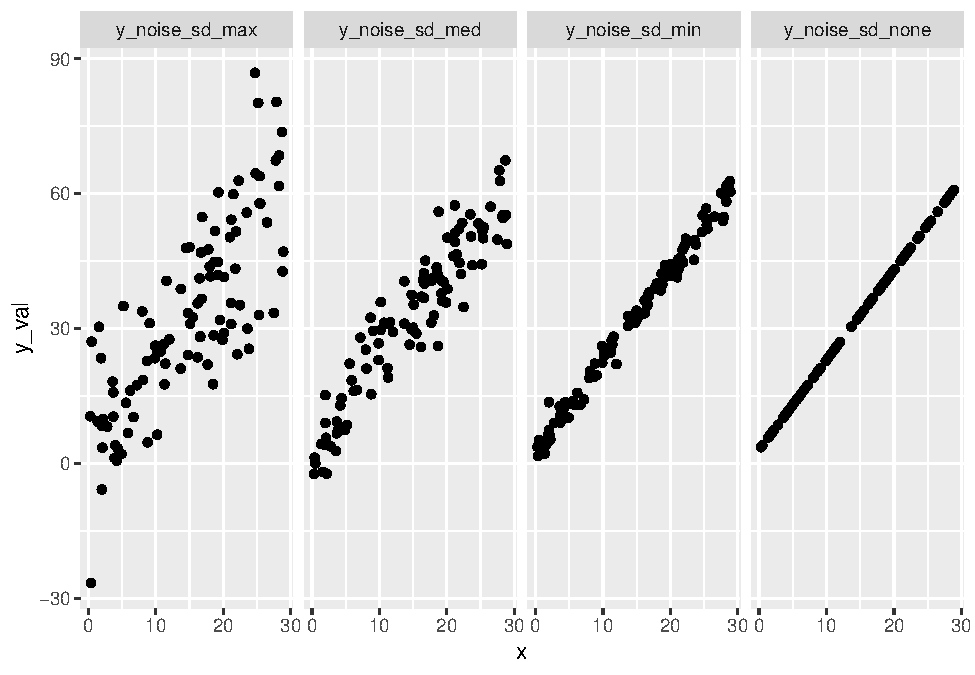
\includegraphics{test_course_notes_files/figure-latex/remedy014-1.pdf}

You can also automatically add in a line with the geom\_smooth() function

\begin{Shaded}
\begin{Highlighting}[]
\NormalTok{demo\_df\_long }\SpecialCharTok{\%\textgreater{}\%} 
  \FunctionTok{ggplot}\NormalTok{(}\FunctionTok{aes}\NormalTok{(}\AttributeTok{x =}\NormalTok{ x, }\AttributeTok{y =}\NormalTok{ y\_val)) }\SpecialCharTok{+}
  \FunctionTok{geom\_point}\NormalTok{() }\SpecialCharTok{+}
  \FunctionTok{geom\_smooth}\NormalTok{(}\AttributeTok{method =} \StringTok{"lm"}\NormalTok{) }\SpecialCharTok{+} 
  \FunctionTok{facet\_grid}\NormalTok{(.}\SpecialCharTok{\textasciitilde{}}\NormalTok{y\_col)}
\end{Highlighting}
\end{Shaded}

\begin{verbatim}
## `geom_smooth()` using formula 'y ~ x'
\end{verbatim}

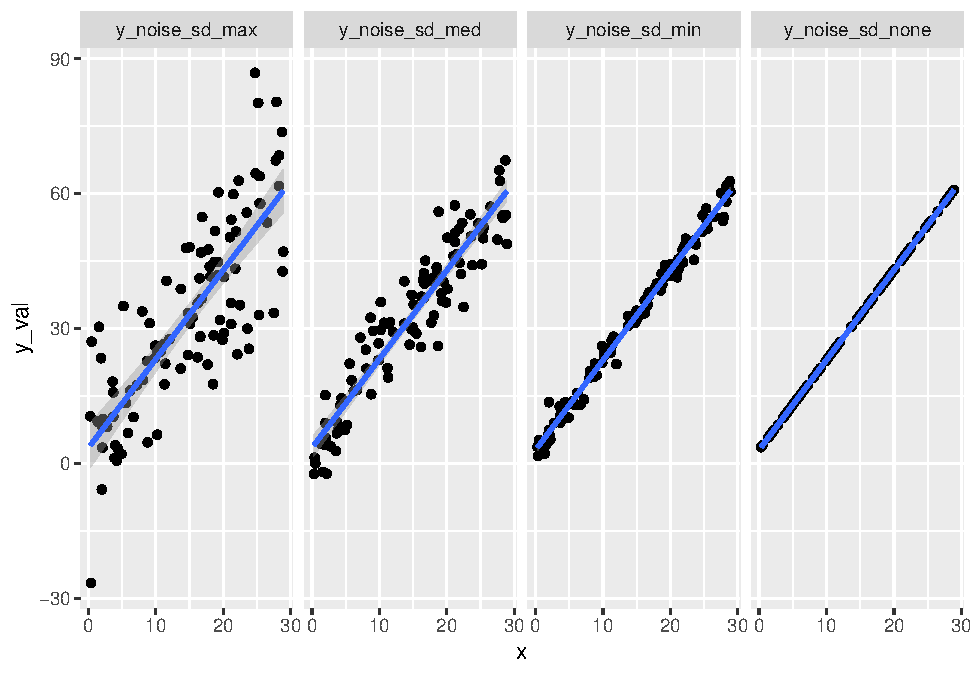
\includegraphics{test_course_notes_files/figure-latex/remedy015-1.pdf}

Now we can create a linear model for the data with minimum noise with the following command:

\begin{Shaded}
\begin{Highlighting}[]
\NormalTok{fit\_demo\_min }\OtherTok{\textless{}{-}} \FunctionTok{lm}\NormalTok{(y\_noise\_sd\_min }\SpecialCharTok{\textasciitilde{}}\NormalTok{ x)}
\end{Highlighting}
\end{Shaded}

\ldots and we can look at the summary of the model with:

\begin{Shaded}
\begin{Highlighting}[]
\FunctionTok{summary}\NormalTok{(fit\_demo\_min)}
\end{Highlighting}
\end{Shaded}

\begin{verbatim}
## 
## Call:
## lm(formula = y_noise_sd_min ~ x)
## 
## Residuals:
##     Min      1Q  Median      3Q     Max 
## -4.8305 -1.0169  0.1167  1.2526  6.6468 
## 
## Coefficients:
##             Estimate Std. Error t value Pr(>|t|)    
## (Intercept)  2.95771    0.38624   7.658 1.35e-11 ***
## x            1.99773    0.02263  88.283  < 2e-16 ***
## ---
## Signif. codes:  0 '***' 0.001 '**' 0.01 '*' 0.05 '.' 0.1 ' ' 1
## 
## Residual standard error: 1.896 on 98 degrees of freedom
## Multiple R-squared:  0.9876, Adjusted R-squared:  0.9875 
## F-statistic:  7794 on 1 and 98 DF,  p-value: < 2.2e-16
\end{verbatim}

We can also look at model results with the glance() function from the broom package

\begin{Shaded}
\begin{Highlighting}[]
\NormalTok{broom}\SpecialCharTok{::}\FunctionTok{glance}\NormalTok{(fit\_demo\_min)}
\end{Highlighting}
\end{Shaded}

\begin{verbatim}
## # A tibble: 1 x 12
##   r.squared adj.r.squared sigma statistic  p.value    df logLik   AIC   BIC
##       <dbl>         <dbl> <dbl>     <dbl>    <dbl> <dbl>  <dbl> <dbl> <dbl>
## 1     0.988         0.987  1.90     7794. 3.28e-95     1  -205.  416.  423.
## # ... with 3 more variables: deviance <dbl>, df.residual <int>, nobs <int>
\end{verbatim}

We can create models for the med and max sd values as well and take a look at those with the summary() function once again

\begin{Shaded}
\begin{Highlighting}[]
\NormalTok{fit\_demo\_med }\OtherTok{\textless{}{-}} \FunctionTok{lm}\NormalTok{(y\_noise\_sd\_med }\SpecialCharTok{\textasciitilde{}}\NormalTok{ x)}
\FunctionTok{summary}\NormalTok{(fit\_demo\_med)}
\end{Highlighting}
\end{Shaded}

\begin{verbatim}
## 
## Call:
## lm(formula = y_noise_sd_med ~ x)
## 
## Residuals:
##      Min       1Q   Median       3Q      Max 
## -14.2828  -4.5096   0.4237   4.4704  15.4196 
## 
## Coefficients:
##             Estimate Std. Error t value Pr(>|t|)    
## (Intercept)  3.44286    1.22498   2.811  0.00597 ** 
## x            1.97540    0.07177  27.525  < 2e-16 ***
## ---
## Signif. codes:  0 '***' 0.001 '**' 0.01 '*' 0.05 '.' 0.1 ' ' 1
## 
## Residual standard error: 6.012 on 98 degrees of freedom
## Multiple R-squared:  0.8855, Adjusted R-squared:  0.8843 
## F-statistic: 757.6 on 1 and 98 DF,  p-value: < 2.2e-16
\end{verbatim}

\begin{Shaded}
\begin{Highlighting}[]
\NormalTok{fit\_demo\_max }\OtherTok{\textless{}{-}} \FunctionTok{lm}\NormalTok{(y\_noise\_sd\_max }\SpecialCharTok{\textasciitilde{}}\NormalTok{ x)}
\FunctionTok{summary}\NormalTok{(fit\_demo\_max)}
\end{Highlighting}
\end{Shaded}

\begin{verbatim}
## 
## Call:
## lm(formula = y_noise_sd_max ~ x)
## 
## Residuals:
##     Min      1Q  Median      3Q     Max 
## -30.799  -8.967   0.468   8.418  34.608 
## 
## Coefficients:
##             Estimate Std. Error t value Pr(>|t|)    
## (Intercept)   3.4076     2.5626    1.33    0.187    
## x             1.9791     0.1501   13.18   <2e-16 ***
## ---
## Signif. codes:  0 '***' 0.001 '**' 0.01 '*' 0.05 '.' 0.1 ' ' 1
## 
## Residual standard error: 12.58 on 98 degrees of freedom
## Multiple R-squared:  0.6394, Adjusted R-squared:  0.6357 
## F-statistic: 173.8 on 1 and 98 DF,  p-value: < 2.2e-16
\end{verbatim}

Notice the increase in the standard error of the coefficient estimates as the noise in y values went up

From a programming perspective, this was not very efficient because I just copied, pasted, and corrected these values.
There is a better way to do this using lists (see below)

Let's do some fancy stuff to make multiple models at once rather than having to write new lines for each model
*Some of these ideas are taken from the R4DS book chapter 25

\begin{Shaded}
\begin{Highlighting}[]
\NormalTok{test\_nest }\OtherTok{\textless{}{-}}\NormalTok{ demo\_df\_long }\SpecialCharTok{\%\textgreater{}\%} \FunctionTok{nest}\NormalTok{(}\AttributeTok{data =} \SpecialCharTok{{-}}\NormalTok{sd\_val)}


\NormalTok{linear\_model }\OtherTok{\textless{}{-}} \ControlFlowTok{function}\NormalTok{(df) \{}
  \FunctionTok{lm}\NormalTok{(y\_val }\SpecialCharTok{\textasciitilde{}}\NormalTok{ x, }\AttributeTok{data =}\NormalTok{ df)}
\NormalTok{\}}


\NormalTok{models }\OtherTok{\textless{}{-}} \FunctionTok{map}\NormalTok{(test\_nest}\SpecialCharTok{$}\NormalTok{data, linear\_model)}
\end{Highlighting}
\end{Shaded}

\begin{Shaded}
\begin{Highlighting}[]
\FunctionTok{summary}\NormalTok{(models[[}\DecValTok{2}\NormalTok{]])}
\end{Highlighting}
\end{Shaded}

\begin{verbatim}
## 
## Call:
## lm(formula = y_val ~ x, data = df)
## 
## Residuals:
##     Min      1Q  Median      3Q     Max 
## -4.8305 -1.0169  0.1167  1.2526  6.6468 
## 
## Coefficients:
##             Estimate Std. Error t value Pr(>|t|)    
## (Intercept)  2.95771    0.38624   7.658 1.35e-11 ***
## x            1.99773    0.02263  88.283  < 2e-16 ***
## ---
## Signif. codes:  0 '***' 0.001 '**' 0.01 '*' 0.05 '.' 0.1 ' ' 1
## 
## Residual standard error: 1.896 on 98 degrees of freedom
## Multiple R-squared:  0.9876, Adjusted R-squared:  0.9875 
## F-statistic:  7794 on 1 and 98 DF,  p-value: < 2.2e-16
\end{verbatim}

\begin{Shaded}
\begin{Highlighting}[]
\FunctionTok{summary}\NormalTok{(models[[}\DecValTok{3}\NormalTok{]])}
\end{Highlighting}
\end{Shaded}

\begin{verbatim}
## 
## Call:
## lm(formula = y_val ~ x, data = df)
## 
## Residuals:
##      Min       1Q   Median       3Q      Max 
## -14.2828  -4.5096   0.4237   4.4704  15.4196 
## 
## Coefficients:
##             Estimate Std. Error t value Pr(>|t|)    
## (Intercept)  3.44286    1.22498   2.811  0.00597 ** 
## x            1.97540    0.07177  27.525  < 2e-16 ***
## ---
## Signif. codes:  0 '***' 0.001 '**' 0.01 '*' 0.05 '.' 0.1 ' ' 1
## 
## Residual standard error: 6.012 on 98 degrees of freedom
## Multiple R-squared:  0.8855, Adjusted R-squared:  0.8843 
## F-statistic: 757.6 on 1 and 98 DF,  p-value: < 2.2e-16
\end{verbatim}

\begin{Shaded}
\begin{Highlighting}[]
\FunctionTok{summary}\NormalTok{(models[[}\DecValTok{4}\NormalTok{]])}
\end{Highlighting}
\end{Shaded}

\begin{verbatim}
## 
## Call:
## lm(formula = y_val ~ x, data = df)
## 
## Residuals:
##     Min      1Q  Median      3Q     Max 
## -30.799  -8.967   0.468   8.418  34.608 
## 
## Coefficients:
##             Estimate Std. Error t value Pr(>|t|)    
## (Intercept)   3.4076     2.5626    1.33    0.187    
## x             1.9791     0.1501   13.18   <2e-16 ***
## ---
## Signif. codes:  0 '***' 0.001 '**' 0.01 '*' 0.05 '.' 0.1 ' ' 1
## 
## Residual standard error: 12.58 on 98 degrees of freedom
## Multiple R-squared:  0.6394, Adjusted R-squared:  0.6357 
## F-statistic: 173.8 on 1 and 98 DF,  p-value: < 2.2e-16
\end{verbatim}

We can also store the models as new columns in the nested dataframe

\begin{Shaded}
\begin{Highlighting}[]
\NormalTok{test\_nest }\OtherTok{\textless{}{-}}\NormalTok{ test\_nest }\SpecialCharTok{\%\textgreater{}\%} 
  \FunctionTok{mutate}\NormalTok{(}\AttributeTok{model =} \FunctionTok{map}\NormalTok{(data, linear\_model))}
\end{Highlighting}
\end{Shaded}

Finally, we can unnest the models to make it easier to compare them with each other in a data frame

\begin{Shaded}
\begin{Highlighting}[]
\NormalTok{test\_nest }\OtherTok{\textless{}{-}}\NormalTok{ test\_nest }\SpecialCharTok{\%\textgreater{}\%} 
  \FunctionTok{mutate}\NormalTok{(}\AttributeTok{glance =} \FunctionTok{map}\NormalTok{(model, broom}\SpecialCharTok{::}\NormalTok{glance)) }\SpecialCharTok{\%\textgreater{}\%} 
  \FunctionTok{unnest}\NormalTok{(glance)}
\end{Highlighting}
\end{Shaded}

\begin{verbatim}
## Warning in summary.lm(x): essentially perfect fit: summary may be unreliable

## Warning in summary.lm(x): essentially perfect fit: summary may be unreliable
\end{verbatim}

\hypertarget{data-generation-demo---one-set-sample-size-1}{%
\section{Data generation demo - one set sample size;}\label{data-generation-demo---one-set-sample-size-1}}

The change from the past demo is that we are now sampling from integer values rather than continuous for the predictor

Store the sample size that we want to use

\begin{Shaded}
\begin{Highlighting}[]
\NormalTok{samp\_size }\OtherTok{\textless{}{-}} \DecValTok{200}
\end{Highlighting}
\end{Shaded}

Instead of sampling uniformly from 0 to 20, this is to sample integers from 40 to 100 uniformly.
We take ``samp\_size'' number of samples. Replace = TRUE means we can get the same x value multiple times

\begin{Shaded}
\begin{Highlighting}[]
\NormalTok{x }\OtherTok{\textless{}{-}} \FunctionTok{sample}\NormalTok{(}\AttributeTok{x =} \FunctionTok{c}\NormalTok{(}\DecValTok{60}\SpecialCharTok{:}\DecValTok{100}\NormalTok{), }\AttributeTok{size =}\NormalTok{ samp\_size, }\AttributeTok{replace =} \ConstantTok{TRUE}\NormalTok{)}
\end{Highlighting}
\end{Shaded}

As before, store the noise values for our different test models

\begin{Shaded}
\begin{Highlighting}[]
\NormalTok{sd\_min }\OtherTok{\textless{}{-}} \DecValTok{2}
\NormalTok{sd\_med }\OtherTok{\textless{}{-}} \DecValTok{6}
\NormalTok{sd\_max }\OtherTok{\textless{}{-}} \DecValTok{12}

\NormalTok{y\_noise\_sd\_none }\OtherTok{\textless{}{-}} \DecValTok{3} \SpecialCharTok{+} \DecValTok{2}\SpecialCharTok{*}\NormalTok{x}
\NormalTok{y\_noise\_sd\_min }\OtherTok{\textless{}{-}} \DecValTok{3} \SpecialCharTok{+} \DecValTok{2}\SpecialCharTok{*}\NormalTok{x }\SpecialCharTok{+} \FunctionTok{round}\NormalTok{(}\AttributeTok{x =} \FunctionTok{rnorm}\NormalTok{(}\AttributeTok{n =}\NormalTok{ samp\_size, }\AttributeTok{mean =} \DecValTok{0}\NormalTok{, }\AttributeTok{sd =}\NormalTok{ sd\_min), }\AttributeTok{digits =} \DecValTok{1}\NormalTok{)}
\NormalTok{y\_noise\_sd\_med }\OtherTok{\textless{}{-}} \DecValTok{3} \SpecialCharTok{+} \DecValTok{2}\SpecialCharTok{*}\NormalTok{x }\SpecialCharTok{+} \FunctionTok{round}\NormalTok{(}\AttributeTok{x =} \FunctionTok{rnorm}\NormalTok{(}\AttributeTok{n =}\NormalTok{ samp\_size, }\AttributeTok{mean =} \DecValTok{0}\NormalTok{, }\AttributeTok{sd =}\NormalTok{ sd\_med), }\AttributeTok{digits =} \DecValTok{1}\NormalTok{)}
\NormalTok{y\_noise\_sd\_max }\OtherTok{\textless{}{-}} \DecValTok{3} \SpecialCharTok{+} \DecValTok{2}\SpecialCharTok{*}\NormalTok{x }\SpecialCharTok{+} \FunctionTok{round}\NormalTok{(}\AttributeTok{x =} \FunctionTok{rnorm}\NormalTok{(}\AttributeTok{n =}\NormalTok{ samp\_size, }\AttributeTok{mean =} \DecValTok{0}\NormalTok{, }\AttributeTok{sd =}\NormalTok{ sd\_max), }\AttributeTok{digits =} \DecValTok{1}\NormalTok{)}
\end{Highlighting}
\end{Shaded}

Typical step 1: visualize! Let's plot each of these x values vs y

\begin{Shaded}
\begin{Highlighting}[]
\FunctionTok{plot}\NormalTok{(x, y\_noise\_sd\_none)}
\end{Highlighting}
\end{Shaded}

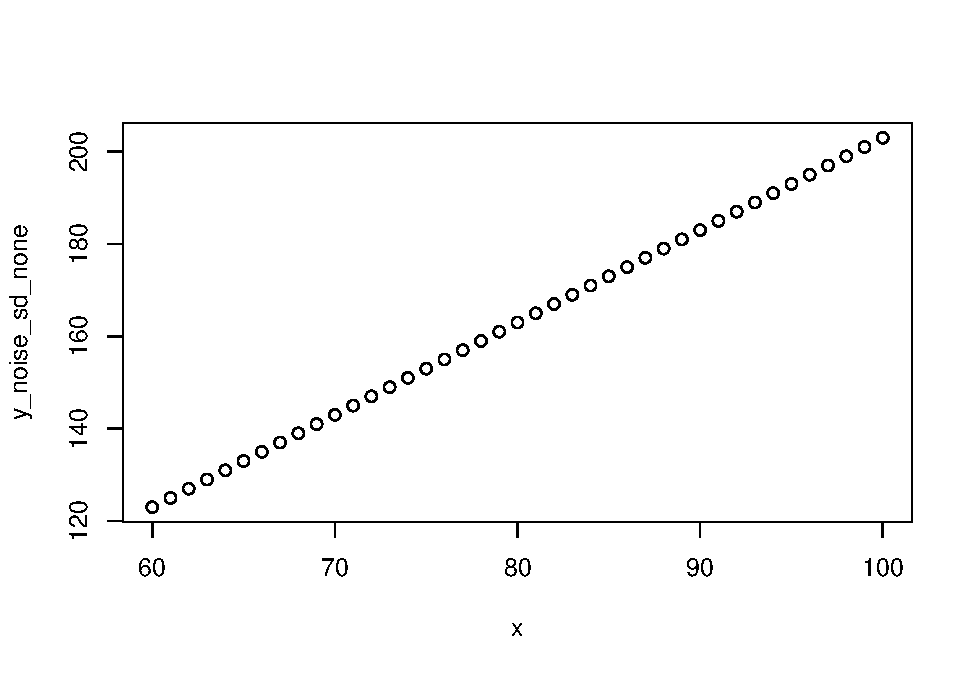
\includegraphics{test_course_notes_files/figure-latex/remedy030-1.pdf}

\begin{Shaded}
\begin{Highlighting}[]
\FunctionTok{plot}\NormalTok{(x, y\_noise\_sd\_min)}
\end{Highlighting}
\end{Shaded}

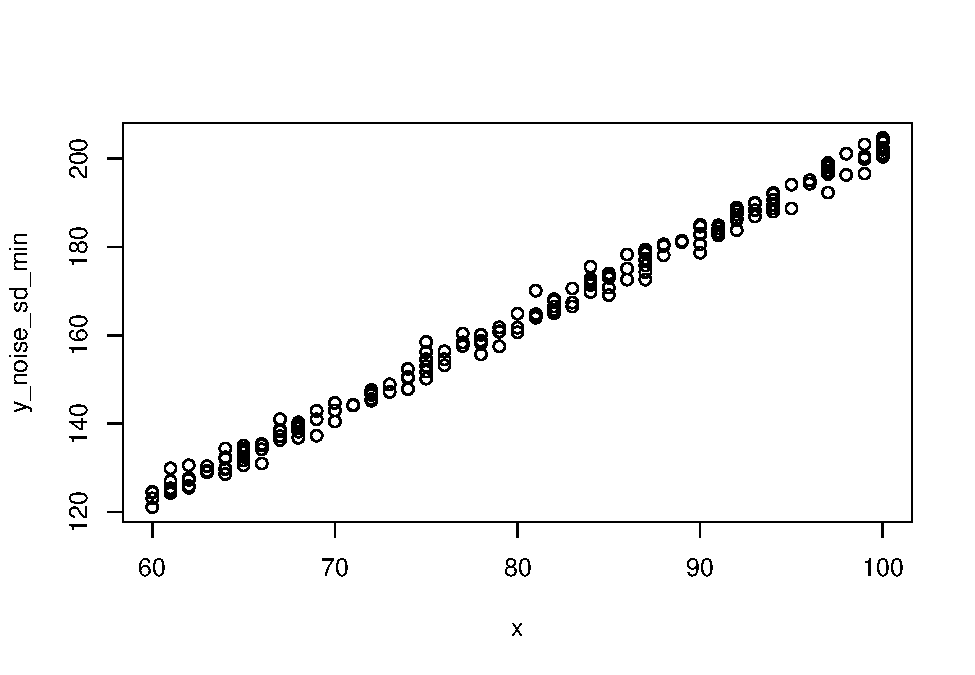
\includegraphics{test_course_notes_files/figure-latex/remedy030-2.pdf}

\begin{Shaded}
\begin{Highlighting}[]
\FunctionTok{plot}\NormalTok{(x, y\_noise\_sd\_med)}
\end{Highlighting}
\end{Shaded}

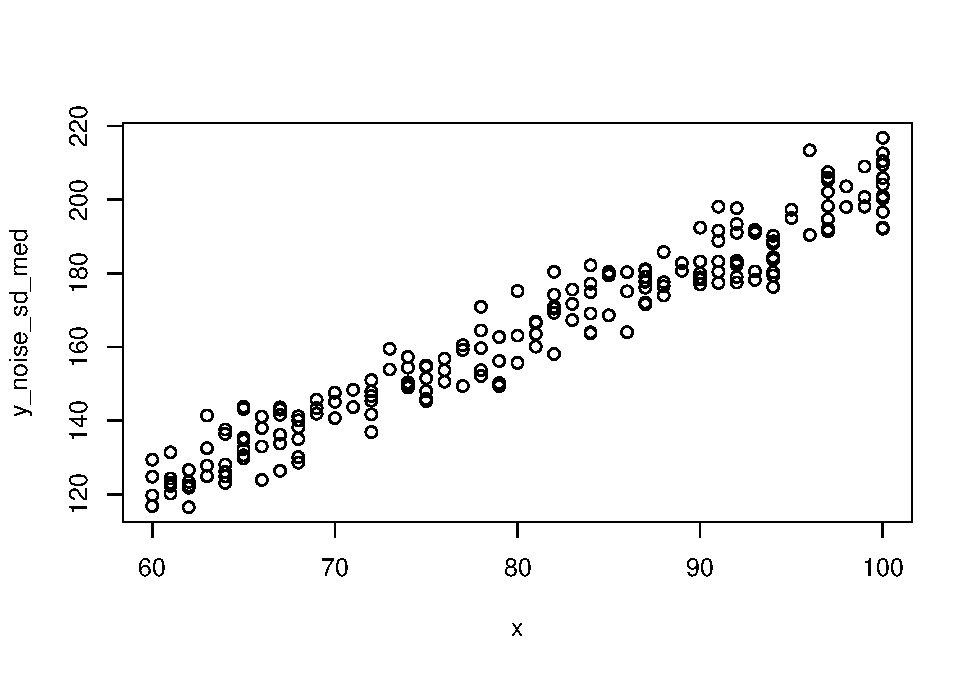
\includegraphics{test_course_notes_files/figure-latex/remedy030-3.pdf}

\begin{Shaded}
\begin{Highlighting}[]
\FunctionTok{plot}\NormalTok{(x, y\_noise\_sd\_max)}
\end{Highlighting}
\end{Shaded}

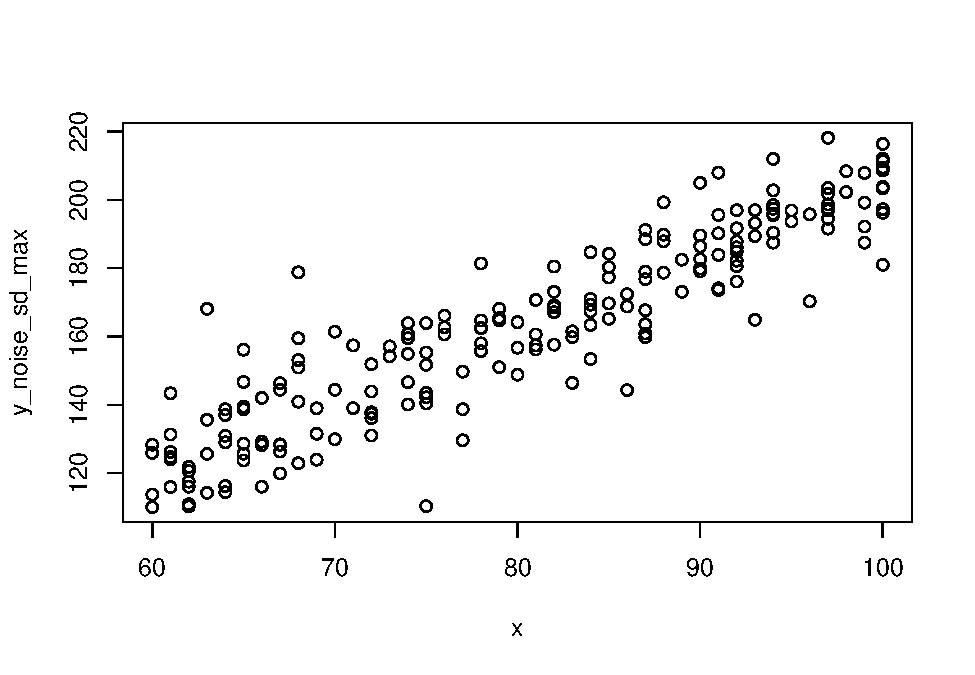
\includegraphics{test_course_notes_files/figure-latex/remedy030-4.pdf}

Let's put all of these vectors together into a data frame to make it easier to analyze later on.
Note, this is not a vital step for conducting the simple regression

\begin{Shaded}
\begin{Highlighting}[]
\NormalTok{demo\_df }\OtherTok{\textless{}{-}} \FunctionTok{tibble}\NormalTok{(}\StringTok{"x"} \OtherTok{=}\NormalTok{ x, }
                  \StringTok{"y\_noise\_sd\_none"}\OtherTok{=}\NormalTok{y\_noise\_sd\_none, }
                  \StringTok{"y\_noise\_sd\_min"} \OtherTok{=}\NormalTok{ y\_noise\_sd\_min,}
                  \StringTok{"y\_noise\_sd\_med"} \OtherTok{=}\NormalTok{ y\_noise\_sd\_med,}
                  \StringTok{"y\_noise\_sd\_max"} \OtherTok{=}\NormalTok{ y\_noise\_sd\_max)}
\end{Highlighting}
\end{Shaded}

Order by increasing x value

\begin{Shaded}
\begin{Highlighting}[]
\NormalTok{demo\_df }\OtherTok{\textless{}{-}}\NormalTok{ demo\_df }\SpecialCharTok{\%\textgreater{}\%} 
  \FunctionTok{arrange}\NormalTok{(x)}
\end{Highlighting}
\end{Shaded}

Let's make this a long df so that we can plot multiple standard deviation values together

\begin{Shaded}
\begin{Highlighting}[]
\NormalTok{demo\_df\_long }\OtherTok{\textless{}{-}}\NormalTok{ demo\_df }\SpecialCharTok{\%\textgreater{}\%} 
  \FunctionTok{pivot\_longer}\NormalTok{(}\AttributeTok{cols =} \FunctionTok{starts\_with}\NormalTok{(}\StringTok{"y\_noise"}\NormalTok{),}
               \AttributeTok{names\_to =} \StringTok{"y\_col"}\NormalTok{,}
               \AttributeTok{values\_to =} \StringTok{"y\_val"}
\NormalTok{  )}
\end{Highlighting}
\end{Shaded}

\begin{Shaded}
\begin{Highlighting}[]
\NormalTok{demo\_df\_long }\OtherTok{\textless{}{-}}\NormalTok{ demo\_df\_long }\SpecialCharTok{\%\textgreater{}\%} 
  \FunctionTok{mutate}\NormalTok{(}\AttributeTok{sd\_val =} \FunctionTok{case\_when}\NormalTok{(}\FunctionTok{str\_detect}\NormalTok{(y\_col, }\StringTok{"sd\_none"}\NormalTok{) }\SpecialCharTok{\textasciitilde{}} \DecValTok{0}\NormalTok{,}
                            \FunctionTok{str\_detect}\NormalTok{(y\_col, }\StringTok{"sd\_min"}\NormalTok{) }\SpecialCharTok{\textasciitilde{}}\NormalTok{ sd\_min,}
                            \FunctionTok{str\_detect}\NormalTok{(y\_col, }\StringTok{"sd\_med"}\NormalTok{) }\SpecialCharTok{\textasciitilde{}}\NormalTok{ sd\_med,}
                            \FunctionTok{str\_detect}\NormalTok{(y\_col, }\StringTok{"sd\_max"}\NormalTok{) }\SpecialCharTok{\textasciitilde{}}\NormalTok{ sd\_max))}
\end{Highlighting}
\end{Shaded}

And visualize the data, faceting by different noise

\begin{Shaded}
\begin{Highlighting}[]
\NormalTok{demo\_df\_long }\SpecialCharTok{\%\textgreater{}\%} 
  \FunctionTok{ggplot}\NormalTok{(}\FunctionTok{aes}\NormalTok{(}\AttributeTok{x =}\NormalTok{ x, }\AttributeTok{y =}\NormalTok{ y\_val)) }\SpecialCharTok{+}
  \FunctionTok{geom\_point}\NormalTok{() }\SpecialCharTok{+}
  \FunctionTok{facet\_grid}\NormalTok{(.}\SpecialCharTok{\textasciitilde{}}\NormalTok{y\_col)}
\end{Highlighting}
\end{Shaded}

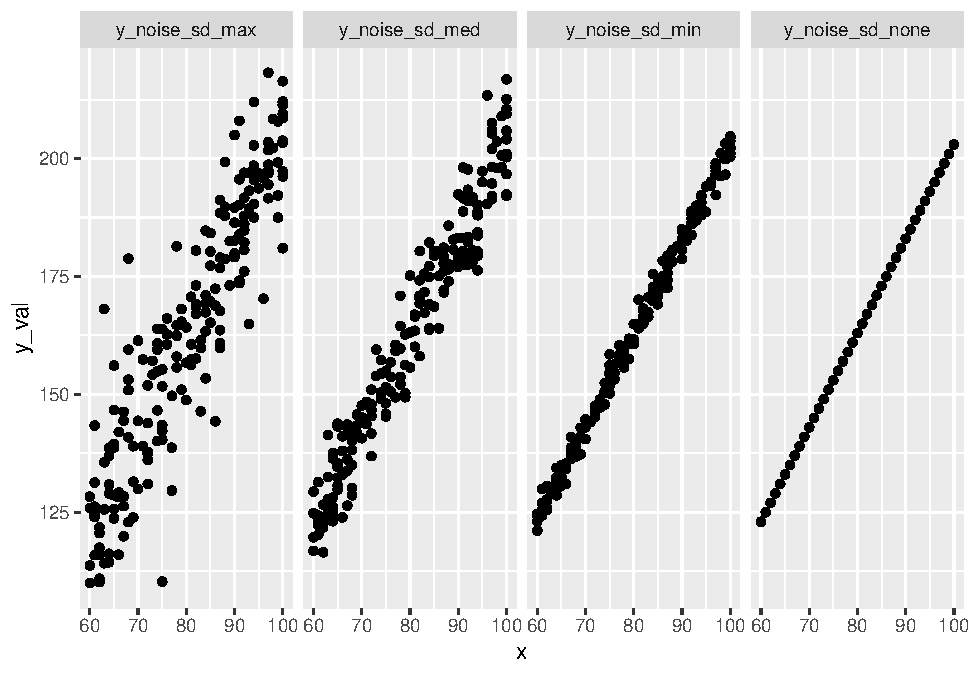
\includegraphics{test_course_notes_files/figure-latex/remedy035-1.pdf}

And add in a line with \texttt{geom\_smooth(method\ =\ \textquotesingle{}lm\textquotesingle{})}

\begin{Shaded}
\begin{Highlighting}[]
\NormalTok{demo\_df\_long }\SpecialCharTok{\%\textgreater{}\%} 
  \FunctionTok{ggplot}\NormalTok{(}\FunctionTok{aes}\NormalTok{(}\AttributeTok{x =}\NormalTok{ x, }\AttributeTok{y =}\NormalTok{ y\_val)) }\SpecialCharTok{+}
  \FunctionTok{geom\_point}\NormalTok{() }\SpecialCharTok{+}
  \FunctionTok{geom\_smooth}\NormalTok{(}\AttributeTok{method =} \StringTok{"lm"}\NormalTok{) }\SpecialCharTok{+} 
  \FunctionTok{facet\_grid}\NormalTok{(.}\SpecialCharTok{\textasciitilde{}}\NormalTok{y\_col)}
\end{Highlighting}
\end{Shaded}

\begin{verbatim}
## `geom_smooth()` using formula 'y ~ x'
\end{verbatim}

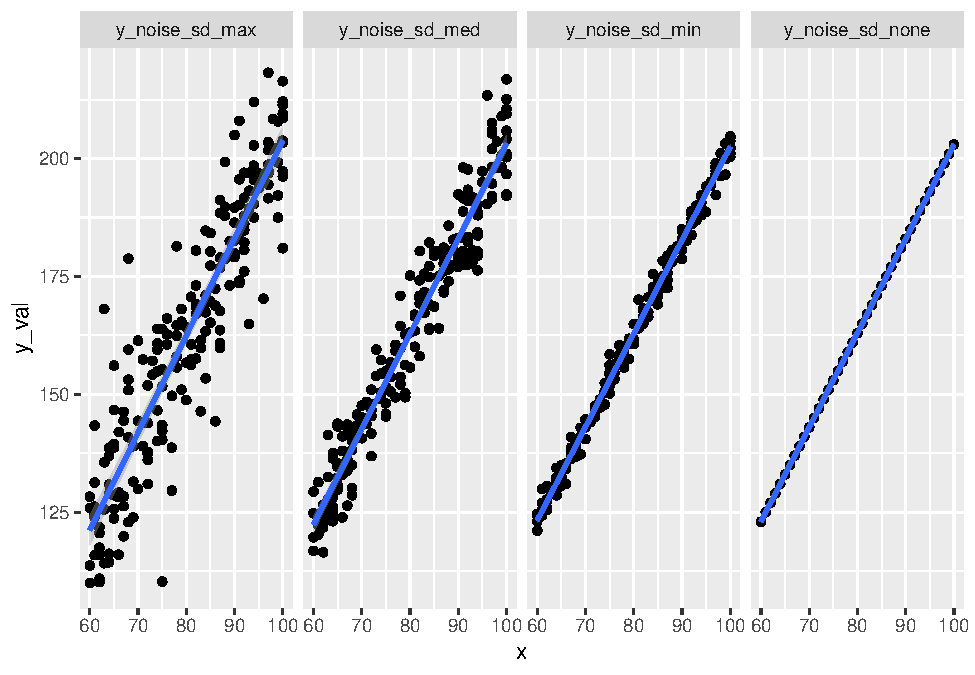
\includegraphics{test_course_notes_files/figure-latex/remedy036-1.pdf}

Create a linear model and look at the summary.

\begin{Shaded}
\begin{Highlighting}[]
\NormalTok{fit\_demo\_min }\OtherTok{\textless{}{-}} \FunctionTok{lm}\NormalTok{(y\_noise\_sd\_min }\SpecialCharTok{\textasciitilde{}}\NormalTok{ x)}
\FunctionTok{summary}\NormalTok{(fit\_demo\_min)}
\end{Highlighting}
\end{Shaded}

\begin{verbatim}
## 
## Call:
## lm(formula = y_noise_sd_min ~ x)
## 
## Residuals:
##    Min     1Q Median     3Q    Max 
## -4.255 -1.179 -0.014  1.292  5.508 
## 
## Coefficients:
##             Estimate Std. Error t value Pr(>|t|)    
## (Intercept)  4.48189    0.85866    5.22 4.51e-07 ***
## x            1.98014    0.01056  187.47  < 2e-16 ***
## ---
## Signif. codes:  0 '***' 0.001 '**' 0.01 '*' 0.05 '.' 0.1 ' ' 1
## 
## Residual standard error: 1.839 on 198 degrees of freedom
## Multiple R-squared:  0.9944, Adjusted R-squared:  0.9944 
## F-statistic: 3.514e+04 on 1 and 198 DF,  p-value: < 2.2e-16
\end{verbatim}

We can also look at model results with the glance() function from the broom package

\begin{Shaded}
\begin{Highlighting}[]
\NormalTok{broom}\SpecialCharTok{::}\FunctionTok{glance}\NormalTok{(fit\_demo\_min)}
\end{Highlighting}
\end{Shaded}

\begin{verbatim}
## # A tibble: 1 x 12
##   r.squared adj.r.squared sigma statistic   p.value    df logLik   AIC   BIC
##       <dbl>         <dbl> <dbl>     <dbl>     <dbl> <dbl>  <dbl> <dbl> <dbl>
## 1     0.994         0.994  1.84    35144. 6.97e-225     1  -405.  815.  825.
## # ... with 3 more variables: deviance <dbl>, df.residual <int>, nobs <int>
\end{verbatim}

We can create models for the med and max sd values as well and take a look at those with the summary() function once again.

\begin{Shaded}
\begin{Highlighting}[]
\NormalTok{fit\_demo\_med }\OtherTok{\textless{}{-}} \FunctionTok{lm}\NormalTok{(y\_noise\_sd\_med }\SpecialCharTok{\textasciitilde{}}\NormalTok{ x)}
\FunctionTok{summary}\NormalTok{(fit\_demo\_med)}
\end{Highlighting}
\end{Shaded}

\begin{verbatim}
## 
## Call:
## lm(formula = y_noise_sd_med ~ x)
## 
## Residuals:
##      Min       1Q   Median       3Q      Max 
## -14.8080  -4.5099  -0.3439   4.0105  18.2525 
## 
## Coefficients:
##             Estimate Std. Error t value Pr(>|t|)    
## (Intercept)  1.25146    2.85726   0.438    0.662    
## x            2.01975    0.03515  57.465   <2e-16 ***
## ---
## Signif. codes:  0 '***' 0.001 '**' 0.01 '*' 0.05 '.' 0.1 ' ' 1
## 
## Residual standard error: 6.12 on 198 degrees of freedom
## Multiple R-squared:  0.9434, Adjusted R-squared:  0.9431 
## F-statistic:  3302 on 1 and 198 DF,  p-value: < 2.2e-16
\end{verbatim}

\begin{Shaded}
\begin{Highlighting}[]
\NormalTok{fit\_demo\_max }\OtherTok{\textless{}{-}} \FunctionTok{lm}\NormalTok{(y\_noise\_sd\_max }\SpecialCharTok{\textasciitilde{}}\NormalTok{ x)}
\FunctionTok{summary}\NormalTok{(fit\_demo\_max)}
\end{Highlighting}
\end{Shaded}

\begin{verbatim}
## 
## Call:
## lm(formula = y_noise_sd_max ~ x)
## 
## Residuals:
##     Min      1Q  Median      3Q     Max 
## -41.873  -7.524   0.032   7.119  41.081 
## 
## Coefficients:
##             Estimate Std. Error t value Pr(>|t|)    
## (Intercept) -2.69072    5.35997  -0.502    0.616    
## x            2.06485    0.06593  31.317   <2e-16 ***
## ---
## Signif. codes:  0 '***' 0.001 '**' 0.01 '*' 0.05 '.' 0.1 ' ' 1
## 
## Residual standard error: 11.48 on 198 degrees of freedom
## Multiple R-squared:  0.832,  Adjusted R-squared:  0.8312 
## F-statistic: 980.8 on 1 and 198 DF,  p-value: < 2.2e-16
\end{verbatim}

Notice the increase in the standard error of the coefficient estimates as the noise in y values went up

From a programming perspective, this was not very efficient because I just copied, pasted, and corrected these values.
There is a better way to do this using lists (see below)

Let's do some fancy stuff to make multiple models at once rather than having to write new lines for each model
*Some of these ideas are taken from the R4DS book chapter 25

\begin{Shaded}
\begin{Highlighting}[]
\NormalTok{test\_nest }\OtherTok{\textless{}{-}}\NormalTok{ demo\_df\_long }\SpecialCharTok{\%\textgreater{}\%} \FunctionTok{nest}\NormalTok{(}\AttributeTok{data =} \SpecialCharTok{{-}}\NormalTok{sd\_val)}


\NormalTok{linear\_model }\OtherTok{\textless{}{-}} \ControlFlowTok{function}\NormalTok{(df) \{}
  \FunctionTok{lm}\NormalTok{(y\_val }\SpecialCharTok{\textasciitilde{}}\NormalTok{ x, }\AttributeTok{data =}\NormalTok{ df)}
\NormalTok{\}}


\NormalTok{models }\OtherTok{\textless{}{-}} \FunctionTok{map}\NormalTok{(test\_nest}\SpecialCharTok{$}\NormalTok{data, linear\_model)}
\end{Highlighting}
\end{Shaded}

\begin{Shaded}
\begin{Highlighting}[]
\FunctionTok{summary}\NormalTok{(models[[}\DecValTok{2}\NormalTok{]])}
\end{Highlighting}
\end{Shaded}

\begin{verbatim}
## 
## Call:
## lm(formula = y_val ~ x, data = df)
## 
## Residuals:
##    Min     1Q Median     3Q    Max 
## -4.255 -1.179 -0.014  1.292  5.508 
## 
## Coefficients:
##             Estimate Std. Error t value Pr(>|t|)    
## (Intercept)  4.48189    0.85866    5.22 4.51e-07 ***
## x            1.98014    0.01056  187.47  < 2e-16 ***
## ---
## Signif. codes:  0 '***' 0.001 '**' 0.01 '*' 0.05 '.' 0.1 ' ' 1
## 
## Residual standard error: 1.839 on 198 degrees of freedom
## Multiple R-squared:  0.9944, Adjusted R-squared:  0.9944 
## F-statistic: 3.514e+04 on 1 and 198 DF,  p-value: < 2.2e-16
\end{verbatim}

\begin{Shaded}
\begin{Highlighting}[]
\FunctionTok{summary}\NormalTok{(models[[}\DecValTok{3}\NormalTok{]])}
\end{Highlighting}
\end{Shaded}

\begin{verbatim}
## 
## Call:
## lm(formula = y_val ~ x, data = df)
## 
## Residuals:
##      Min       1Q   Median       3Q      Max 
## -14.8080  -4.5099  -0.3439   4.0105  18.2525 
## 
## Coefficients:
##             Estimate Std. Error t value Pr(>|t|)    
## (Intercept)  1.25146    2.85726   0.438    0.662    
## x            2.01975    0.03515  57.465   <2e-16 ***
## ---
## Signif. codes:  0 '***' 0.001 '**' 0.01 '*' 0.05 '.' 0.1 ' ' 1
## 
## Residual standard error: 6.12 on 198 degrees of freedom
## Multiple R-squared:  0.9434, Adjusted R-squared:  0.9431 
## F-statistic:  3302 on 1 and 198 DF,  p-value: < 2.2e-16
\end{verbatim}

\begin{Shaded}
\begin{Highlighting}[]
\FunctionTok{summary}\NormalTok{(models[[}\DecValTok{4}\NormalTok{]])}
\end{Highlighting}
\end{Shaded}

\begin{verbatim}
## 
## Call:
## lm(formula = y_val ~ x, data = df)
## 
## Residuals:
##     Min      1Q  Median      3Q     Max 
## -41.873  -7.524   0.032   7.119  41.081 
## 
## Coefficients:
##             Estimate Std. Error t value Pr(>|t|)    
## (Intercept) -2.69072    5.35997  -0.502    0.616    
## x            2.06485    0.06593  31.317   <2e-16 ***
## ---
## Signif. codes:  0 '***' 0.001 '**' 0.01 '*' 0.05 '.' 0.1 ' ' 1
## 
## Residual standard error: 11.48 on 198 degrees of freedom
## Multiple R-squared:  0.832,  Adjusted R-squared:  0.8312 
## F-statistic: 980.8 on 1 and 198 DF,  p-value: < 2.2e-16
\end{verbatim}

We can also store the models as new columns in the nested dataframe

\begin{Shaded}
\begin{Highlighting}[]
\NormalTok{test\_nest }\OtherTok{\textless{}{-}}\NormalTok{ test\_nest }\SpecialCharTok{\%\textgreater{}\%} 
  \FunctionTok{mutate}\NormalTok{(}\AttributeTok{model =} \FunctionTok{map}\NormalTok{(data, linear\_model))}
\end{Highlighting}
\end{Shaded}

Finally, we can unnest the models to make it easier to compare them with each other in a data frame

\begin{Shaded}
\begin{Highlighting}[]
\NormalTok{test\_nest }\OtherTok{\textless{}{-}}\NormalTok{ test\_nest }\SpecialCharTok{\%\textgreater{}\%} 
  \FunctionTok{mutate}\NormalTok{(}\AttributeTok{glance =} \FunctionTok{map}\NormalTok{(model, broom}\SpecialCharTok{::}\NormalTok{glance)) }\SpecialCharTok{\%\textgreater{}\%} 
  \FunctionTok{unnest}\NormalTok{(glance)}
\end{Highlighting}
\end{Shaded}

\hypertarget{data-generation-with-three-different-sample-sizes}{%
\section{Data generation with three different sample sizes}\label{data-generation-with-three-different-sample-sizes}}

Let's run the same demo but now have three different sample sizes - 10, 50, and 500

First, store the sample sizes we want to use

\begin{Shaded}
\begin{Highlighting}[]
\NormalTok{samp\_sizes }\OtherTok{\textless{}{-}} \FunctionTok{c}\NormalTok{(}\DecValTok{10}\NormalTok{, }\DecValTok{50}\NormalTok{, }\DecValTok{500}\NormalTok{)}
\end{Highlighting}
\end{Shaded}

Next, create a bookkeping column for ourselves to keep track of which sample size the future values will come from

\begin{Shaded}
\begin{Highlighting}[]
\NormalTok{samp\_size\_col }\OtherTok{\textless{}{-}} \FunctionTok{rep}\NormalTok{(}\AttributeTok{x =} \FunctionTok{c}\NormalTok{(}\DecValTok{10}\NormalTok{,}\DecValTok{50}\NormalTok{, }\DecValTok{500}\NormalTok{), }\AttributeTok{times =}\NormalTok{ samp\_sizes)}
\end{Highlighting}
\end{Shaded}

Calculate the total number of values we will need from the three samples combined

\begin{Shaded}
\begin{Highlighting}[]
\NormalTok{tot\_samp\_size }\OtherTok{\textless{}{-}} \FunctionTok{sum}\NormalTok{(samp\_sizes)}
\end{Highlighting}
\end{Shaded}

Sample uniformly from 0 to 20

\begin{Shaded}
\begin{Highlighting}[]
\NormalTok{x }\OtherTok{\textless{}{-}} \FunctionTok{round}\NormalTok{(}\AttributeTok{x =} \FunctionTok{runif}\NormalTok{(}\AttributeTok{n =}\NormalTok{ tot\_samp\_size, }\AttributeTok{min =} \DecValTok{0}\NormalTok{, }\AttributeTok{max =} \DecValTok{20}\NormalTok{), }\AttributeTok{digits =} \DecValTok{1}\NormalTok{)}
\end{Highlighting}
\end{Shaded}

Store the standard deviations for the min, med, and max models

\begin{Shaded}
\begin{Highlighting}[]
\NormalTok{sd\_min }\OtherTok{\textless{}{-}} \DecValTok{2}
\NormalTok{sd\_med }\OtherTok{\textless{}{-}} \DecValTok{6}
\NormalTok{sd\_max }\OtherTok{\textless{}{-}} \DecValTok{12}
\end{Highlighting}
\end{Shaded}

Calculate the y values for the different scenarios where there is no noise up to max noise

\begin{Shaded}
\begin{Highlighting}[]
\NormalTok{y\_noise\_sd\_none }\OtherTok{\textless{}{-}} \DecValTok{3} \SpecialCharTok{+} \DecValTok{2}\SpecialCharTok{*}\NormalTok{x}
\NormalTok{y\_noise\_sd\_min }\OtherTok{\textless{}{-}} \DecValTok{3} \SpecialCharTok{+} \DecValTok{2}\SpecialCharTok{*}\NormalTok{x }\SpecialCharTok{+} \FunctionTok{round}\NormalTok{(}\AttributeTok{x =} \FunctionTok{rnorm}\NormalTok{(}\AttributeTok{n =}\NormalTok{ tot\_samp\_size, }\AttributeTok{mean =} \DecValTok{0}\NormalTok{, }\AttributeTok{sd =}\NormalTok{ sd\_min), }\AttributeTok{digits =} \DecValTok{1}\NormalTok{)}
\NormalTok{y\_noise\_sd\_med }\OtherTok{\textless{}{-}} \DecValTok{3} \SpecialCharTok{+} \DecValTok{2}\SpecialCharTok{*}\NormalTok{x }\SpecialCharTok{+} \FunctionTok{round}\NormalTok{(}\AttributeTok{x =} \FunctionTok{rnorm}\NormalTok{(}\AttributeTok{n =}\NormalTok{ tot\_samp\_size, }\AttributeTok{mean =} \DecValTok{0}\NormalTok{, }\AttributeTok{sd =}\NormalTok{ sd\_med), }\AttributeTok{digits =} \DecValTok{1}\NormalTok{)}
\NormalTok{y\_noise\_sd\_max }\OtherTok{\textless{}{-}} \DecValTok{3} \SpecialCharTok{+} \DecValTok{2}\SpecialCharTok{*}\NormalTok{x }\SpecialCharTok{+} \FunctionTok{round}\NormalTok{(}\AttributeTok{x =} \FunctionTok{rnorm}\NormalTok{(}\AttributeTok{n =}\NormalTok{ tot\_samp\_size, }\AttributeTok{mean =} \DecValTok{0}\NormalTok{, }\AttributeTok{sd =}\NormalTok{ sd\_max), }\AttributeTok{digits =} \DecValTok{1}\NormalTok{)}
\end{Highlighting}
\end{Shaded}

Typical step 1: visualize! Let's plot each of these x values vs y

\begin{Shaded}
\begin{Highlighting}[]
\FunctionTok{plot}\NormalTok{(x, y\_noise\_sd\_none)}
\end{Highlighting}
\end{Shaded}

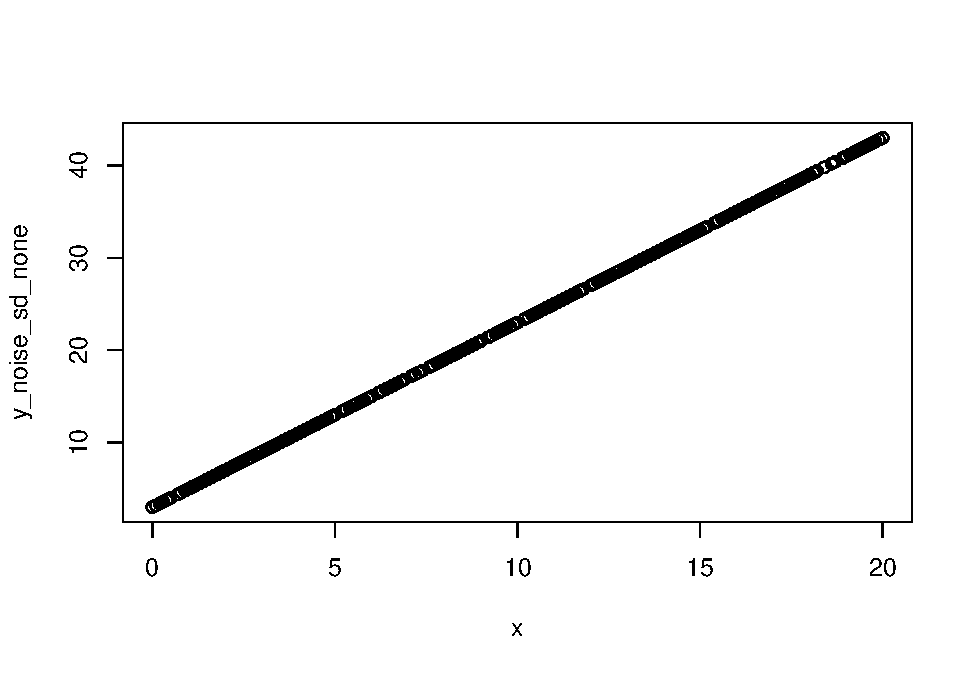
\includegraphics{test_course_notes_files/figure-latex/unnamed-chunk-80-1.pdf}

\begin{Shaded}
\begin{Highlighting}[]
\FunctionTok{plot}\NormalTok{(x, y\_noise\_sd\_min)}
\end{Highlighting}
\end{Shaded}

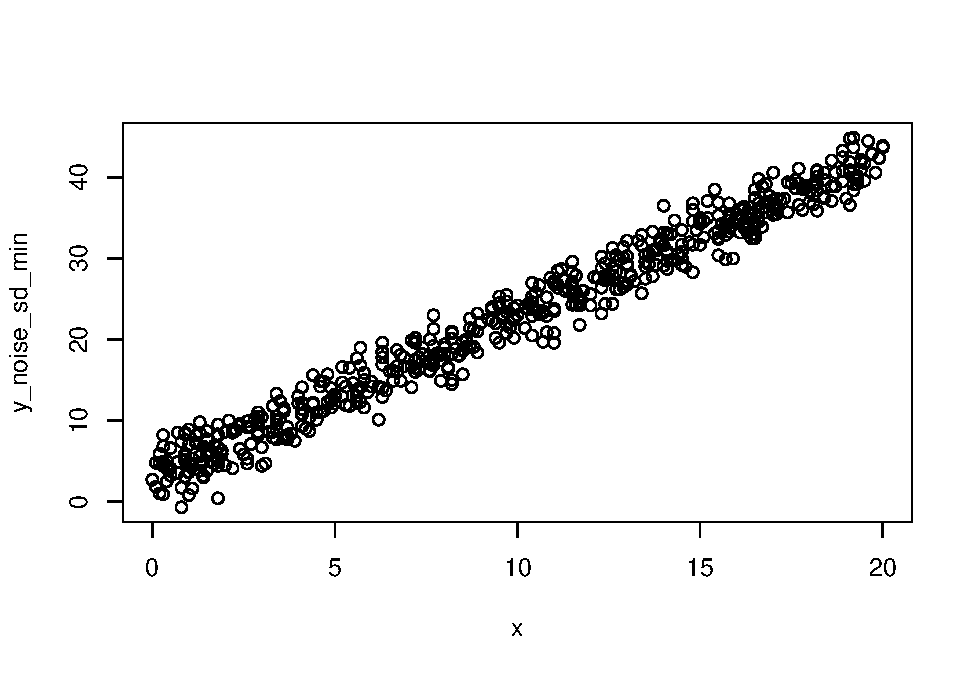
\includegraphics{test_course_notes_files/figure-latex/unnamed-chunk-80-2.pdf}

\begin{Shaded}
\begin{Highlighting}[]
\FunctionTok{plot}\NormalTok{(x, y\_noise\_sd\_med)}
\end{Highlighting}
\end{Shaded}

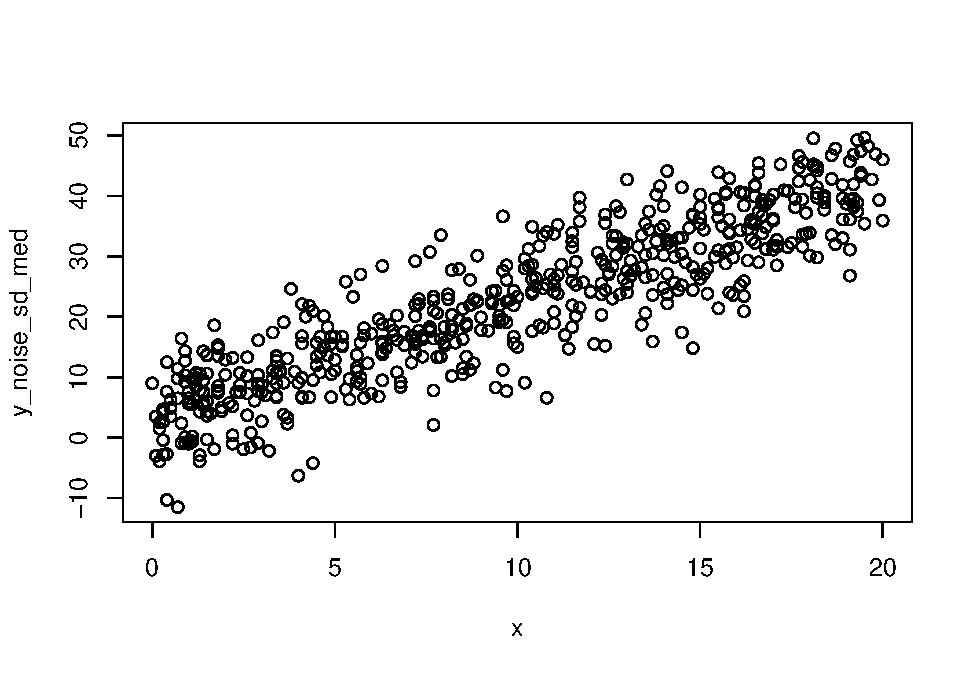
\includegraphics{test_course_notes_files/figure-latex/unnamed-chunk-80-3.pdf}

\begin{Shaded}
\begin{Highlighting}[]
\FunctionTok{plot}\NormalTok{(x, y\_noise\_sd\_max)}
\end{Highlighting}
\end{Shaded}

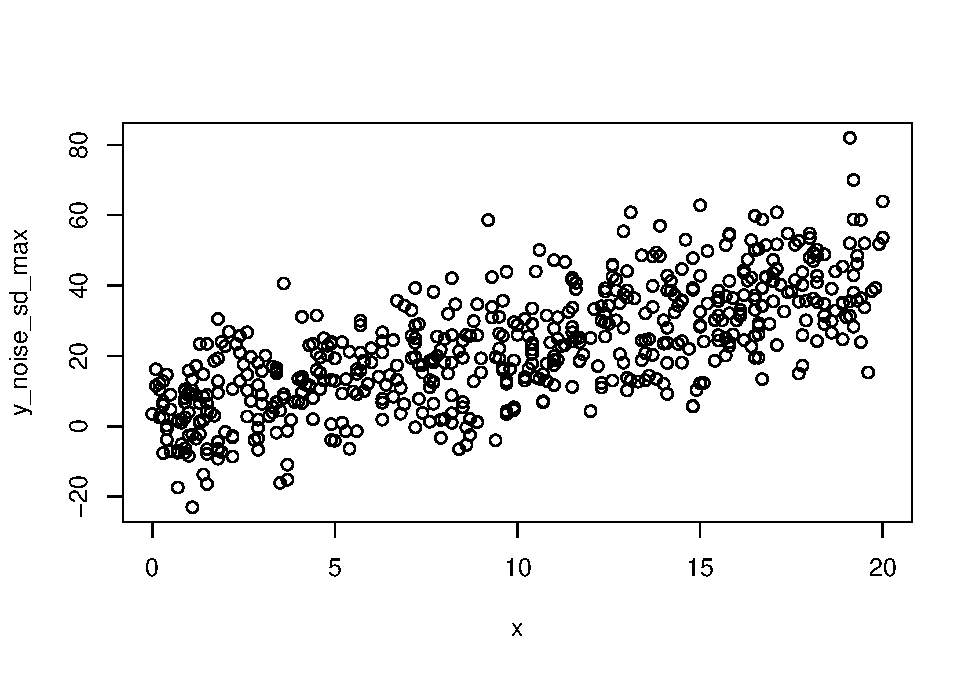
\includegraphics{test_course_notes_files/figure-latex/unnamed-chunk-80-4.pdf}
Can we calculate the correlations between x and these different y values? (pro tip: yes)

Let's put all of these vectors together into a data frame to make it easier to analyze later on
Note, this is not a vital step for conducting the simple regression

\begin{Shaded}
\begin{Highlighting}[]
\NormalTok{demo\_df }\OtherTok{\textless{}{-}} \FunctionTok{tibble}\NormalTok{(}\StringTok{"n"} \OtherTok{=}\NormalTok{ samp\_size\_col,}
                  \StringTok{"x"} \OtherTok{=}\NormalTok{ x, }
                  \StringTok{"y\_noise\_sd\_none"}\OtherTok{=}\NormalTok{y\_noise\_sd\_none, }
                  \StringTok{"y\_noise\_sd\_min"} \OtherTok{=}\NormalTok{ y\_noise\_sd\_min,}
                  \StringTok{"y\_noise\_sd\_med"} \OtherTok{=}\NormalTok{ y\_noise\_sd\_med,}
                  \StringTok{"y\_noise\_sd\_max"} \OtherTok{=}\NormalTok{ y\_noise\_sd\_max)}
\end{Highlighting}
\end{Shaded}

Order by increasing x value

\begin{Shaded}
\begin{Highlighting}[]
\NormalTok{demo\_df }\OtherTok{\textless{}{-}}\NormalTok{ demo\_df }\SpecialCharTok{\%\textgreater{}\%} 
  \FunctionTok{arrange}\NormalTok{(n, x)}
\end{Highlighting}
\end{Shaded}

Let's make this a long df so that we can plot multiple standard deviation values together

\begin{Shaded}
\begin{Highlighting}[]
\NormalTok{demo\_df\_long }\OtherTok{\textless{}{-}}\NormalTok{ demo\_df }\SpecialCharTok{\%\textgreater{}\%} 
  \FunctionTok{pivot\_longer}\NormalTok{(}\AttributeTok{cols =} \FunctionTok{starts\_with}\NormalTok{(}\StringTok{"y\_noise"}\NormalTok{),}
               \AttributeTok{names\_to =} \StringTok{"y\_col"}\NormalTok{,}
               \AttributeTok{values\_to =} \StringTok{"y\_val"}
\NormalTok{  )}

\NormalTok{demo\_df\_long }\OtherTok{\textless{}{-}}\NormalTok{ demo\_df\_long }\SpecialCharTok{\%\textgreater{}\%} 
  \FunctionTok{mutate}\NormalTok{(}\AttributeTok{sd\_val =} \FunctionTok{case\_when}\NormalTok{(}\FunctionTok{str\_detect}\NormalTok{(y\_col, }\StringTok{"sd\_none"}\NormalTok{) }\SpecialCharTok{\textasciitilde{}} \DecValTok{0}\NormalTok{,}
                            \FunctionTok{str\_detect}\NormalTok{(y\_col, }\StringTok{"sd\_min"}\NormalTok{) }\SpecialCharTok{\textasciitilde{}}\NormalTok{ sd\_min,}
                            \FunctionTok{str\_detect}\NormalTok{(y\_col, }\StringTok{"sd\_med"}\NormalTok{) }\SpecialCharTok{\textasciitilde{}}\NormalTok{ sd\_med,}
                            \FunctionTok{str\_detect}\NormalTok{(y\_col, }\StringTok{"sd\_max"}\NormalTok{) }\SpecialCharTok{\textasciitilde{}}\NormalTok{ sd\_max))}
\end{Highlighting}
\end{Shaded}

\begin{Shaded}
\begin{Highlighting}[]
\NormalTok{demo\_df\_long }\SpecialCharTok{\%\textgreater{}\%} 
  \FunctionTok{ggplot}\NormalTok{(}\FunctionTok{aes}\NormalTok{(}\AttributeTok{x =}\NormalTok{ x, }\AttributeTok{y =}\NormalTok{ y\_val)) }\SpecialCharTok{+}
  \FunctionTok{geom\_point}\NormalTok{() }\SpecialCharTok{+}
  \FunctionTok{facet\_grid}\NormalTok{(n}\SpecialCharTok{\textasciitilde{}}\NormalTok{y\_col)}
\end{Highlighting}
\end{Shaded}

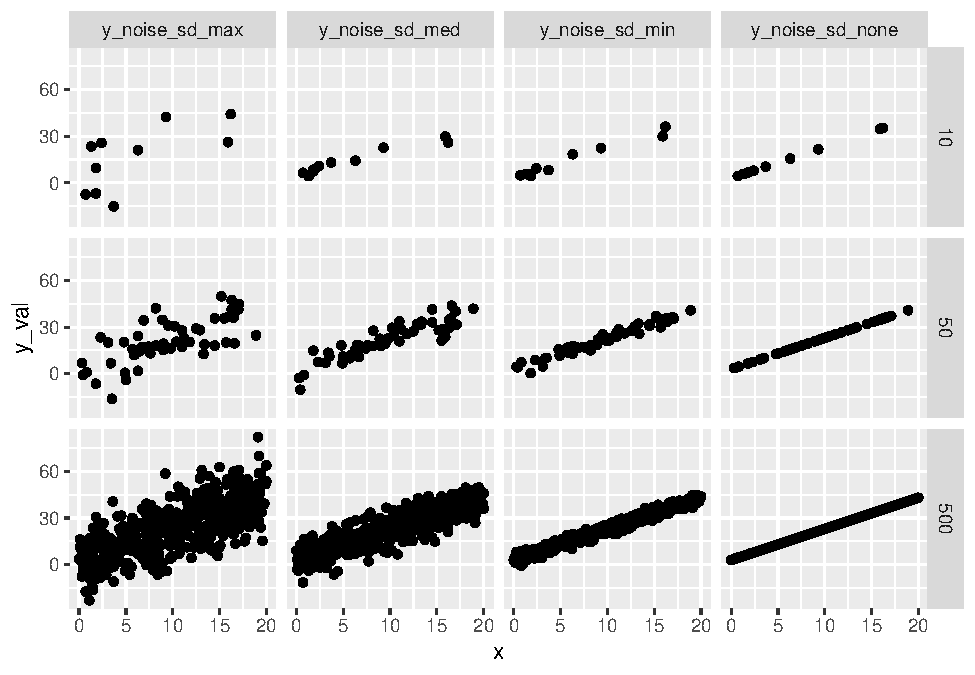
\includegraphics{test_course_notes_files/figure-latex/unnamed-chunk-84-1.pdf}

\begin{Shaded}
\begin{Highlighting}[]
\NormalTok{demo\_df\_long }\SpecialCharTok{\%\textgreater{}\%} 
  \FunctionTok{ggplot}\NormalTok{(}\FunctionTok{aes}\NormalTok{(}\AttributeTok{x =}\NormalTok{ x, }\AttributeTok{y =}\NormalTok{ y\_val)) }\SpecialCharTok{+}
  \FunctionTok{geom\_point}\NormalTok{() }\SpecialCharTok{+}
  \FunctionTok{geom\_smooth}\NormalTok{(}\AttributeTok{method =} \StringTok{"lm"}\NormalTok{) }\SpecialCharTok{+} 
  \FunctionTok{facet\_grid}\NormalTok{(n}\SpecialCharTok{\textasciitilde{}}\NormalTok{y\_col)}
\end{Highlighting}
\end{Shaded}

\begin{verbatim}
## `geom_smooth()` using formula 'y ~ x'
\end{verbatim}

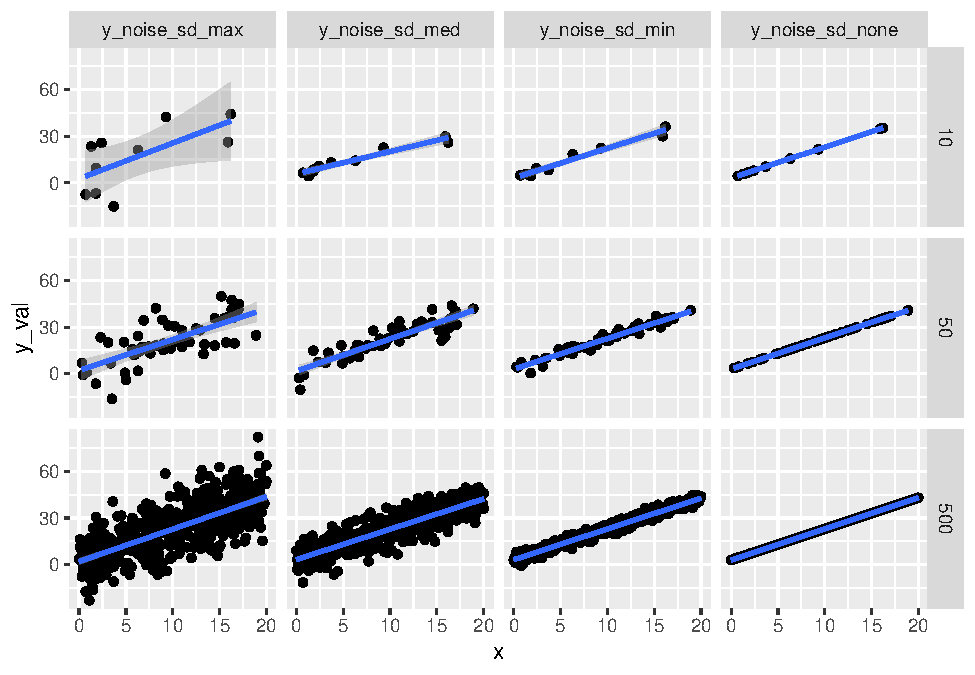
\includegraphics{test_course_notes_files/figure-latex/unnamed-chunk-85-1.pdf}

\begin{Shaded}
\begin{Highlighting}[]
\NormalTok{fit\_demo\_min }\OtherTok{\textless{}{-}} \FunctionTok{lm}\NormalTok{(y\_noise\_sd\_min }\SpecialCharTok{\textasciitilde{}}\NormalTok{ x)}
\FunctionTok{summary}\NormalTok{(fit\_demo\_min)}
\end{Highlighting}
\end{Shaded}

\begin{verbatim}
## 
## Call:
## lm(formula = y_noise_sd_min ~ x)
## 
## Residuals:
##     Min      1Q  Median      3Q     Max 
## -6.2890 -1.2959  0.0241  1.3551  5.6700 
## 
## Coefficients:
##             Estimate Std. Error t value Pr(>|t|)    
## (Intercept)  3.12724    0.16334   19.15   <2e-16 ***
## x            1.97877    0.01437  137.74   <2e-16 ***
## ---
## Signif. codes:  0 '***' 0.001 '**' 0.01 '*' 0.05 '.' 0.1 ' ' 1
## 
## Residual standard error: 1.991 on 558 degrees of freedom
## Multiple R-squared:  0.9714, Adjusted R-squared:  0.9714 
## F-statistic: 1.897e+04 on 1 and 558 DF,  p-value: < 2.2e-16
\end{verbatim}

\hypertarget{can-also-look-at-model-results-with-the-glance-function-from-the-broom-package}{%
\chapter{can also look at model results with the glance() function from the broom package}\label{can-also-look-at-model-results-with-the-glance-function-from-the-broom-package}}

\begin{Shaded}
\begin{Highlighting}[]
\NormalTok{broom}\SpecialCharTok{::}\FunctionTok{glance}\NormalTok{(fit\_demo\_min)}
\end{Highlighting}
\end{Shaded}

\begin{verbatim}
## # A tibble: 1 x 12
##   r.squared adj.r.squared sigma statistic p.value    df logLik   AIC   BIC
##       <dbl>         <dbl> <dbl>     <dbl>   <dbl> <dbl>  <dbl> <dbl> <dbl>
## 1     0.971         0.971  1.99    18971.       0     1 -1179. 2365. 2378.
## # ... with 3 more variables: deviance <dbl>, df.residual <int>, nobs <int>
\end{verbatim}

We can create models for the med and max sd values as well and take a look at those with the summary() function once again

\begin{Shaded}
\begin{Highlighting}[]
\NormalTok{fit\_demo\_med }\OtherTok{\textless{}{-}} \FunctionTok{lm}\NormalTok{(y\_noise\_sd\_med }\SpecialCharTok{\textasciitilde{}}\NormalTok{ x)}
\FunctionTok{summary}\NormalTok{(fit\_demo\_med)}
\end{Highlighting}
\end{Shaded}

\begin{verbatim}
## 
## Call:
## lm(formula = y_noise_sd_med ~ x)
## 
## Residuals:
##      Min       1Q   Median       3Q      Max 
## -17.6985  -3.7966   0.2362   3.8811  14.8663 
## 
## Coefficients:
##             Estimate Std. Error t value Pr(>|t|)    
## (Intercept)   3.2022     0.4832   6.627 8.09e-11 ***
## x             1.9534     0.0425  45.960  < 2e-16 ***
## ---
## Signif. codes:  0 '***' 0.001 '**' 0.01 '*' 0.05 '.' 0.1 ' ' 1
## 
## Residual standard error: 5.89 on 558 degrees of freedom
## Multiple R-squared:  0.791,  Adjusted R-squared:  0.7907 
## F-statistic:  2112 on 1 and 558 DF,  p-value: < 2.2e-16
\end{verbatim}

\begin{Shaded}
\begin{Highlighting}[]
\NormalTok{fit\_demo\_max }\OtherTok{\textless{}{-}} \FunctionTok{lm}\NormalTok{(y\_noise\_sd\_max }\SpecialCharTok{\textasciitilde{}}\NormalTok{ x)}
\FunctionTok{summary}\NormalTok{(fit\_demo\_max)}
\end{Highlighting}
\end{Shaded}

\begin{verbatim}
## 
## Call:
## lm(formula = y_noise_sd_max ~ x)
## 
## Residuals:
##     Min      1Q  Median      3Q     Max 
## -27.424  -8.335  -0.024   7.614  40.314 
## 
## Coefficients:
##             Estimate Std. Error t value Pr(>|t|)    
## (Intercept)  2.02590    0.95825   2.114   0.0349 *  
## x            2.07643    0.08428  24.637   <2e-16 ***
## ---
## Signif. codes:  0 '***' 0.001 '**' 0.01 '*' 0.05 '.' 0.1 ' ' 1
## 
## Residual standard error: 11.68 on 558 degrees of freedom
## Multiple R-squared:  0.521,  Adjusted R-squared:  0.5202 
## F-statistic:   607 on 1 and 558 DF,  p-value: < 2.2e-16
\end{verbatim}

Notice the increase in the standard error of the coefficient estimates as the noise in y values went up

From a programming perspective, this was not very efficient because I just copied, pasted, and corrected these values.
There is a better way to do this using lists (see below)

Let's do some fancy stuff to make multiple models at once rather than having to write new lines for each model
*Some of these ideas are taken from the R4DS book chapter 25

\begin{Shaded}
\begin{Highlighting}[]
\NormalTok{test\_nest }\OtherTok{\textless{}{-}}\NormalTok{ demo\_df\_long }\SpecialCharTok{\%\textgreater{}\%} \FunctionTok{nest}\NormalTok{(}\AttributeTok{data =} \SpecialCharTok{{-}}\FunctionTok{c}\NormalTok{(sd\_val, n))}


\NormalTok{linear\_model }\OtherTok{\textless{}{-}} \ControlFlowTok{function}\NormalTok{(df) \{}
  \FunctionTok{lm}\NormalTok{(y\_val }\SpecialCharTok{\textasciitilde{}}\NormalTok{ x, }\AttributeTok{data =}\NormalTok{ df)}
\NormalTok{\}}


\NormalTok{models }\OtherTok{\textless{}{-}} \FunctionTok{map}\NormalTok{(test\_nest}\SpecialCharTok{$}\NormalTok{data, linear\_model)}

\FunctionTok{summary}\NormalTok{(models[[}\DecValTok{2}\NormalTok{]])}
\end{Highlighting}
\end{Shaded}

\begin{verbatim}
## 
## Call:
## lm(formula = y_val ~ x, data = df)
## 
## Residuals:
##     Min      1Q  Median      3Q     Max 
## -3.5563 -1.7545  0.2615  1.5699  3.2498 
## 
## Coefficients:
##             Estimate Std. Error t value Pr(>|t|)    
## (Intercept)   3.0712     1.0479   2.931    0.019 *  
## x             1.9173     0.1281  14.972 3.91e-07 ***
## ---
## Signif. codes:  0 '***' 0.001 '**' 0.01 '*' 0.05 '.' 0.1 ' ' 1
## 
## Residual standard error: 2.279 on 8 degrees of freedom
## Multiple R-squared:  0.9655, Adjusted R-squared:  0.9612 
## F-statistic: 224.2 on 1 and 8 DF,  p-value: 3.91e-07
\end{verbatim}

\begin{Shaded}
\begin{Highlighting}[]
\FunctionTok{summary}\NormalTok{(models[[}\DecValTok{3}\NormalTok{]])}
\end{Highlighting}
\end{Shaded}

\begin{verbatim}
## 
## Call:
## lm(formula = y_val ~ x, data = df)
## 
## Residuals:
##     Min      1Q  Median      3Q     Max 
## -3.3114 -0.8539 -0.0393  1.4128  3.4565 
## 
## Coefficients:
##             Estimate Std. Error t value Pr(>|t|)    
## (Intercept)   5.7375     1.0549   5.439 0.000617 ***
## x             1.4415     0.1289  11.181 3.67e-06 ***
## ---
## Signif. codes:  0 '***' 0.001 '**' 0.01 '*' 0.05 '.' 0.1 ' ' 1
## 
## Residual standard error: 2.294 on 8 degrees of freedom
## Multiple R-squared:  0.9399, Adjusted R-squared:  0.9323 
## F-statistic:   125 on 1 and 8 DF,  p-value: 3.666e-06
\end{verbatim}

\begin{Shaded}
\begin{Highlighting}[]
\FunctionTok{summary}\NormalTok{(models[[}\DecValTok{4}\NormalTok{]])}
\end{Highlighting}
\end{Shaded}

\begin{verbatim}
## 
## Call:
## lm(formula = y_val ~ x, data = df)
## 
## Residuals:
##     Min      1Q  Median      3Q     Max 
## -26.345 -12.703   3.303  14.251  18.417 
## 
## Coefficients:
##             Estimate Std. Error t value Pr(>|t|)  
## (Intercept)   2.6617     7.6081   0.350    0.735  
## x             2.2926     0.9298   2.466    0.039 *
## ---
## Signif. codes:  0 '***' 0.001 '**' 0.01 '*' 0.05 '.' 0.1 ' ' 1
## 
## Residual standard error: 16.55 on 8 degrees of freedom
## Multiple R-squared:  0.4318, Adjusted R-squared:  0.3608 
## F-statistic:  6.08 on 1 and 8 DF,  p-value: 0.03897
\end{verbatim}

We can also store the models as new columns in the nested dataframe

\begin{Shaded}
\begin{Highlighting}[]
\NormalTok{test\_nest }\OtherTok{\textless{}{-}}\NormalTok{ test\_nest }\SpecialCharTok{\%\textgreater{}\%} 
  \FunctionTok{mutate}\NormalTok{(}\AttributeTok{model =} \FunctionTok{map}\NormalTok{(data, linear\_model))}
\end{Highlighting}
\end{Shaded}

Finally, we can unnest the models to make it easier to compare them with each other in a data frame

\begin{Shaded}
\begin{Highlighting}[]
\NormalTok{test\_nest }\OtherTok{\textless{}{-}}\NormalTok{ test\_nest }\SpecialCharTok{\%\textgreater{}\%} 
  \FunctionTok{mutate}\NormalTok{(}\AttributeTok{glance =} \FunctionTok{map}\NormalTok{(model, broom}\SpecialCharTok{::}\NormalTok{glance)) }\SpecialCharTok{\%\textgreater{}\%} 
  \FunctionTok{unnest}\NormalTok{(glance)}
\end{Highlighting}
\end{Shaded}

\begin{verbatim}
## Warning in summary.lm(x): essentially perfect fit: summary may be unreliable

## Warning in summary.lm(x): essentially perfect fit: summary may be unreliable

## Warning in summary.lm(x): essentially perfect fit: summary may be unreliable

## Warning in summary.lm(x): essentially perfect fit: summary may be unreliable

## Warning in summary.lm(x): essentially perfect fit: summary may be unreliable

## Warning in summary.lm(x): essentially perfect fit: summary may be unreliable
\end{verbatim}

And look at the different models by just calling the data frame

\begin{Shaded}
\begin{Highlighting}[]
\NormalTok{test\_nest}
\end{Highlighting}
\end{Shaded}

\begin{verbatim}
## # A tibble: 12 x 16
##        n sd_val data  model r.squared adj.r.squared    sigma statistic   p.value
##    <dbl>  <dbl> <lis> <lis>     <dbl>         <dbl>    <dbl>     <dbl>     <dbl>
##  1    10      0 <tib~ <lm>      1             1     6.50e-15   3.00e31 1.38e-123
##  2    10      2 <tib~ <lm>      0.966         0.961 2.28e+ 0   2.24e 2 3.91e-  7
##  3    10      6 <tib~ <lm>      0.940         0.932 2.29e+ 0   1.25e 2 3.67e-  6
##  4    10     12 <tib~ <lm>      0.432         0.361 1.65e+ 1   6.08e 0 3.90e-  2
##  5    50      0 <tib~ <lm>      1             1     7.31e-16   9.52e33 0.       
##  6    50      2 <tib~ <lm>      0.955         0.954 2.21e+ 0   1.01e 3 7.02e- 34
##  7    50      6 <tib~ <lm>      0.805         0.801 5.23e+ 0   1.98e 2 1.19e- 18
##  8    50     12 <tib~ <lm>      0.487         0.476 1.05e+ 1   4.56e 1 1.78e-  8
##  9   500      0 <tib~ <lm>      1             1     1.35e-14   3.85e32 0.       
## 10   500      2 <tib~ <lm>      0.973         0.973 1.97e+ 0   1.77e 4 0.       
## 11   500      6 <tib~ <lm>      0.788         0.788 5.99e+ 0   1.85e 3 4.90e-170
## 12   500     12 <tib~ <lm>      0.525         0.524 1.17e+ 1   5.50e 2 1.54e- 82
## # ... with 7 more variables: df <dbl>, logLik <dbl>, AIC <dbl>, BIC <dbl>,
## #   deviance <dbl>, df.residual <int>, nobs <int>
\end{verbatim}

\hypertarget{week-6-regression-ii}{%
\chapter{Week 6: Regression II}\label{week-6-regression-ii}}

This is where the Week 6 magic happens\ldots{}

  \bibliography{book.bib,packages.bib}

\end{document}
